\PassOptionsToPackage{table}{xcolor}
\documentclass[12pt,onesided]{amsart} 
\usepackage{natbib}
\usepackage{amsmath}
\usepackage{pifont}
\usepackage[multiple]{footmisc}
\usepackage{subfigure}
\usepackage[T1]{fontenc}
\usepackage{xcolor}
\usepackage{multirow,multicol}
\usepackage{caption}
\usepackage{booktabs}
\usepackage{color}
\usepackage{setspace}
\usepackage{colortbl}
\usepackage{changebar}
\usepackage{dcolumn}
\usepackage{graphicx}
\usepackage{tikz}
\usepackage[section]{placeins}
\setkeys{Gin}{width=\linewidth,totalheight=\textheight,keepaspectratio}
\graphicspath{{graphics/}{../graphics/}}

\usepackage{hyperref}

\usepackage{geometry}
\geometry{verbose,tmargin=1in,bmargin=1in,lmargin=1in,rmargin=1in}
\usepackage{booktabs}
\usepackage{units}
\usepackage{fancyvrb}
\fvset{fontsize=\normalsize}
\usepackage{lipsum}

\usepackage{footnote}
\usepackage{url} 
% \usepackage[nolists,tablesfirst]{endfloat} % places floats at end
\usepackage{nameref}

\begin{document}

%\maketitle
\thispagestyle{empty}

\begin{center}
{\sc \large Contingent Institutions: \\ The Reputational Impact of Investor-State Disputes}
\end{center}

\vspace{20mm}

\begin{quote}
\noindent \textbf{Abstract}. To what extent do alleged violations of international commitments damage state reputation? This paper explores this question with specific reference to investor-state disputes arising under the protection of international investment agreements. Existing theory assumes that institutionalization of international commitments raises the ex post costs of defection, including reputational damage, thereby creating strong incentives for state compliance. We modify this expectation by arguing that the reputational consequences of treaty violations are contingent on institutional rules and information flows. Drawing on a replication of prior research linking investor-state disputes with reduced FDI as well as an original analysis of their impact on investment reputation, we show that the impact of investor-state disputes has been relatively marginal over the 1987-2011 time period, with reputational effects only beginning to materialize in recent years. This temporal variation reflects changes in the rules governing the transparency of international arbitral tribunals as well as expanded media coverage of investment disputes. The central implication of these findings for the broader body of literature on international institutions is that reputational mechanisms for effective treaty enforcement cannot be taken as given but are heavily contingent on institutional design and associated information costs. 
\end{quote}
 
\vspace{10mm}

\begin{center}
Word Count: 7,984
\end{center}

\newpage

\setcounter{page}{1}
\doublespacing

\section*{Introduction}

Research on the compliance of states with international commitments emphasizes the deterrent effect of reputational damage. The underlying assumption is that reneging on a formal commitment damages a state's reputation and jeopardizes future opportunities for international cooperation. Agreements that institutionalize state commitments are consequently expected to constrain state actors from engaging in uncooperative behavior as well as to induce other sets of actors to monitor and punish defections. The idea has gained particular traction in the study of international economic instruments, including debt contracts, investment treaties, and free trade agreements,\footnote{See, for example, \citet{simmons:2000}; \citet{tomz:2007}; \citet{buthe:milner:2014}; \citet{buthe:milner:2008}; \citet{allee:peinhardt:2011}; \citet{elkins:etal:2006}.} but it has also been applied to a broader range of international issues.\footnote{See, for example, \citet{fearon:1997} and \citet{simmons:danner:2010}.}

Somewhat surprisingly, however, the argument linking reputational concerns to compliance with formal agreements remains largely unexamined. Reputational damage has been inferred from evidence of shifting patterns of foreign lending or investment flows.\footnote{See \citet{tomz:2007} and \citet{allee:peinhardt:2011}.} Reputational indicators have also been utilized to explain state entry into formal international agreements as well as defection from them.\footnote{For recent explananations of treaty formation see \citet{elkins:etal:2006} and \citet{simmons:danner:2010}, and for defection \citet{allee:peinhardt:2011} and \citet{freeman:2013}.}  But prior research has not systematically explored the consequences of reneging on commitments for state reputation. This paper fills this gap by exploring the reputational impact of investor-state disputes arising under the protection of bilateral investment treaties (BITs) and other international investment agreements (IIAs).

Investment treaties, which are designed to attract foreign direct investment (FDI) by offering credible property rights protection to private sector actors, have become an increasingly important part of the international legal architecture. As of the end of 2012, 200 states had signed one or more of these agreements, with the total IIA universe approaching 4,000, including 2,857 BITS and 339 other agreements with investment provisions.\footnote{\citet{unctad:2013}} In most cases these IIAs not only formalize commitments to treat foreign investors fairly and equitably, but also include provisions giving investors the right to take investor-state disputes to international arbitration, out of range of the host country's legal system. According to a recent survey, 93 percent of BITs include such provisions, which are intended to guarantee investors that their claims will be adjudicated in an independent, impartial, and timely manner.\footnote{\citet{gaukordger:gordon:2012}: 8} Over the past two decades these provisions have led to a significant proliferation of investor-state dispute settlement (ISDS) cases.

As of the end of 2013, the United Nations Conference on Trade and Development (UNCTAD) had identified 514 treaty-based arbitrations of investor-state disputes involving 98 different nations;\footnote{\citet{unctad:2014}: 1} however, as arbitration often proceeds confidentially, the accuracy of the UNCTAD data is open to question and cannot be fully verified on the basis of other sources. What is known is that the predominant player in international investor-state disputes is the International Centre for the Settlement of International Disputes (ICSID), which is formally affiliated with the World Bank. The ICSID maintains public records of all of the international investment conflicts brought to it for resolution, the number of which totaled 459 as of December 31, 2013.\footnote{\citet{icsid:2014}: 7-8} Drawing on these records as well as data collected by UNCTAD, we create an original database to analyze how alleged treaty violations affect the reputation of states with the international investment community. 

In contrast to the theoretical claims developed in prior research, we argue that the reputational consequences of treaty violations are contingent on institutional design and associated information costs. Central characteristics of the ISDS process, particularly, its narrow, decentralized, uncertain, and untransparent monitoring and enforcement mechanisms have limited its effectiveness by failing to provide international investors with the information they require to update their perceptions of investment risk in a particular country. This situation has recently begun to change in response to increased institutional transparency and growing media coverage; but in accordance with the logic of North's seminal work on institutions, creating an effective system of investment treaty monitoring and enforcement has been a long, slow process.\footnote{\citet{north1990institutions}: 60} Thus whereas prior research has simply assumed that investor claims of treaty violations entail significant costs, our empirical analysis suggests that reputational mechanisms for the enforcement of international commitments are contingent on information flows.

% The first part of the paper offers a brief overview of investor-state dispute settlement (ISDS) with central emphasis on the ICSID. The second section summarizes the basic argument regarding the importance of reputational concerns for sustaining international cooperation and outlines its central limitations, which revolve around its vagueness with respect to the causal linkages between defection from international commitments and state reputation. In the third section we attempt to replicate prior research indicating that involvement in investor-state dispute arbitration reduces FDI inflows and demonstrate that the evidence is singularly uncompelling. The fourth section turns to a more direct method of assessing the consequences of investment disputes and outlines our central research hypotheses, research design, data, and statistical methodology. The subsequent section draws upon two different types of models to explore the reputational costs of investment disputes. We conclude by comparing and contrasting the findings of the analysis with existing understandings of the efficacy of international commitments and their significance for a state's reputation with the international investment community.

\section*{The Investor-State Dispute Settlement Process}

The dominant player in the international investor-state dispute settlement process is the ICSID, which was established as an autonomous international institution under a multilateral treaty drawn up by the executive directors of the World Bank in 1965. As of late 2013, a total of 158 states had ratified the ICSID Convention, not counting Bolivia, Ecuador, and Venezuela, which withdrew from membership between 2007 and 2012.\footnote{\citet{icsid:2014b}}  Prior to December 31, 2013, other notable non-members included Brazil, India, Iran, Iraq, Poland, and South Africa. Several of these nations, however, have agreed to arbitration under the ICSID's Affiliated Facility (AF), which provides for dispute arbitration and conciliation if one of the parties is a citizen of a member state. 

% is open to dispute arbitration and conciliation if one of the parties is a citizen of a member state. As of December 2013, 43 of the total of 459 investor-state disputes brought to the ICSID were arbitrated under the AF rules.\footnote{Ibid: 8}

The central purpose of the ICSID is to facilitate international flows of private investment by removing non-commercial risks and providing investors with access to impartial and flexible dispute settlement procedures. Under Article 25 of the ICSID Convention, the jurisdiction of the center extends to any legal dispute arising directly out of an investment between a contracting state and a national of another contracting state, providing the parties to the dispute consent in writing to ICSID arbitration. Once the parties accede to ICSID jurisdiction, neither can unilaterally withdraw nor refuse to enforce the ICSID arbitral award. Under Article 43, arbitration can only be discontinued if the parties agree to a settlement or dispute withdrawal, which has occurred in approximately 35 percent of all ICSID disputes.\footnote{\citet{icsid:2014}: 13} Parties to investment disputes have the right to appeal for an annulment of arbitral settlements within the ICSID framework, although annulment is extremely unusual. Of the 180 awards rendered by the ICSID as of the end of 2013, only 13 resulted in a partial or full award annulment.\footnote{Ibid: 17}

The bases of consent that are invoked to establish ICSID jurisdiction in an investor-state dispute vary widely. BITs, which have been cited in 63 percent of ICSID arbitral claims, represent the single most important source, followed by investment contracts between states and foreign investors (19 percent), host state investment law (8 percent), free trade agreements (4.5 percent), and multi-lateral investment agreements (5.5 percent).\footnote{Ibid: 10} The ICSID also offers administrative assistance to arbitrations conducted under the rules of the United Nations Commission on International Trade Law (UNCITRAL) as well as to other venues for arbitral settlement, including the International Chamber of Commerce, the London Court of International Arbitration, the Permanent Court of Arbitration, the Cairo Regional Centre for International Commercial Arbitration, and the Arbitration Institute of the Stockholm Chamber of Commerce.

During its first two decades of existence, the ICSID played a relatively limited role, but that situation began to change with the expansion of foreign direct investment and bilateral investment treaties in the 1990s. Reliable information on arbitrations conducted outside of the ICSID framework is limited, but according to UNCTAD's list of 390 disputes for the 1987-2010 period, 245 were arbitrated by the ICSID, 109 by ad hoc panels under the UNCITRAL arbitral rules, and the remainder by the International Chamber of Commerce or other venues.\footnote{\citet{unctad:2011}: 2} These data almost certainly understate the number of disputes that have been internationally arbitrated as well as the role of the ICSID. A case-by-case analysis indicates that the UNCTAD database misses 18 ICSID cases for the 1987-2010 period. UNCTAD records for the 2010 and 2011 also point to the growing importance of the ICSID, which was involved in 74.7 percent of all investment disputes in those two years.\footnote{See \citet{unctad:2011}: 1-2 and \citet{unctad:2012}: 1.}

The significance of the ICSID, however, cannot be defined merely in terms of the number of cases that have come under its jurisdiction. Also of importance are its visibility as an institution formally affiliated with the World Bank and the scope of its legal authority. Under the ICSID Convention, awards are binding on the parties to a dispute and enforceable as if they were final awards of national courts, with the ICSID's narrowly delimited annulment rules establishing the only avenue of appeal. Awards can thus be enforced in any country that adheres to the ICSID Convention. Moreover, unlike other international arbitration bodies, the ICSID maintains a public record of arbitral claims, making information about allegations of investment treaty violations available to the international community. Arbitration in alternative venues is unlikely to have similar consequences, especially if the parties to the dispute remain anonymous and the outcome confidential, which appears to be the case with a significant number of investment disputes. For this reason, investor-state dispute arbitration within the ICSID framework is often assumed to carry high reputational costs, creating incentives for states to capitulate to foreign investor demands.\footnote{\citet{trakman:2013}: 619}  We explore this claim below, drawing upon data both for the ICSID as well as other ISDS venues.

\section*{The Political Economy of State Reputation}

Prior research in political economy has highlighted the importance of reputation for understanding the willingness of governments to comply with their international agreements. In Tomz's influential formulation, reputation establishes the basis for cooperation in a world of uncertainty, shifting preferences, and international anarchy.\footnote{\citet{tomz:2007}} Governments honor their debts and private investors lend money to foreigners because of reputational concerns rather than other potential types of sanctioning mechanisms. Focusing on commitment and compliance in international monetary affairs, Simmons develops a similar line of argument: ``The acceptance of treaty obligations raises expectations about behavior that, once made, are reputationally costly for governments to violate.''\footnote{\citet{simmons:2000}: 819} \citeauthor{buthe:milner:2008} cite reputational effects to argue that international trade agreements provide mechanisms for making credible commitments to foreign investors: ``Violating an institutionalized commitment -- or not making amends to correct a violation that has occurred -- damages a country's reputation for keeping commitments, making future cooperation on the same and other issues more difficult and maybe impossible to achieve.''\footnote{\citet{buthe:milner:2008}: 746}  \citeauthor{buthe:milner:2009} and \citeauthor{elkins:etal:2006} utilize the same logic to explain why bilateral investment treaties represent credible commitments to foreign investors.\footnote{See \citet{buthe:milner:2009} and \citet{elkins:etal:2006}.}

The existing literature thus suggests that by raising ex post reputational costs, formal international commitments create incentives for state compliance. The implication is that high levels of compliance with international agreements are indicative of high reputational costs, whereas low levels of compliance are likely to be observed where reputational costs are low. Arguments emphasizing the importance of reputation also run from compliance to government reputation as illustrated by Allee and Peinhart's analysis of the impact of investor-state disputes.\footnote{\citet{allee:peinhardt:2011}} Similarly, in his study of the interwar period, Tomz finds that ``lemons'' who signal a low regard for foreign commitments lost access to international credit markets.\footnote{\citet{tomz:2007}: 86-94} Thus not only are potential reputational costs assumed to cause compliance with international commitments; real reputational damage is the expected consequence of defection from those commitments. Logically the latter is the key causal issue. If compliance failures do not affect reputation, then reputational concerns are unlikely to yield much in the way of compliance.

For this reason, the subsequent analysis concentrates on exploring the direct reputational impact of alleged compliance failures. Prior research has largely sidestepped this issue, analyzing instead outcomes, such as FDI flows, that are presumed, but never actually shown, to be linked with reputation. In contrast, we explicitly test the impact of alleged defections from international investment treaties on state reputation with specific emphasis on investment reputation. As suggested by \citeauthor{brewster:2009}, existing theoretical accounts of the importance of reputation err on the side of vagueness, ignoring a number of obvious questions.\footnote{\citet{brewster:2009}} How do we define and measure reputation? Whose reputation matters, with whom, and reputation for what? A negative reputation for compliance with agreements on human rights or the environment can obviously coexist with a positive reputation for complying with loan contracts. Likewise, reputations within particular issue domains are of varying importance to different audiences. The international human rights community may attempt to bring a government's behavior into compliance with international norms by ``shaming and blaming'', but its activities are unlikely to affect that government's observance of the rules of the World Trade Organization. The mechanisms through which the monitoring and enforcement of international commitments occurs also vary widely across international institutions and issue domains,\footnote{\citet{gaukordger:gordon:2012}} presumably making some types of commitments more costly to break than others. By focusing specifically on a government's reputation for protecting international investors, we can minimize these difficulties and open the door to more effective theorizing about role of reputation in international political economy.

Our central point of theoretical departure is the established literature on investment treaties, which creates the expectation that allegations of a government's failure to comply with its commitments generate reputational costs, regardless of the findings of arbitral tribunals. According to \citeauthor{schwenzer:hachem:2011}, for example, ``the reputation of a State may be damaged by wrongfully initiated investment treaty arbitration against the State. Such harm to reputation may have quite severe financial consequences for the entire economy of the State concerned.''\footnote{\citet{schwenzer:hachem:2011}: 426} Likewise, in their research on the ICSID, \citeauthor{allee:peinhardt:2011} claim that, ``The filing of a case before ICSID immediately brands the respondent country as an actor that is hostile to investors''\footnote{\citet{allee:peinhardt:2011}: 414} and leads to ``substantial losses in FDI.''\footnote{Ibid: 429} A recent analysis of investment arbitration, likewise argues that ``when an investor commences an ICSID arbitration against a respondent state and the investor ultimately loses, the state may have a credible argument that its `investment reputation' has been unfairly tarnished.''\footnote{\citet{parish2011awarding}: 236} State actors share this view as evidenced by Turkey's request in Europe Cement \& Trade S.A. v. Turkey for ``an award of monetary compensation for the moral damage it has suffered to its reputation and international standing through the bringing of a claim that is baseless and founded on fabricated documents.''\footnote{Europe Cement Investment \& Trade S.A. v. Republic of Turkey. 2009. ICSID Case No. ARB(AF)/07/02: 177} 

While these arguments sound plausible, they fail to take into account the importance of institutional variation. As emphasized both by the literature on international law\footnote{\citet{staton2011judicial}; \citet{cavallaro2008reevaluating}; \citet{guzman2008reputation}; \citet{guzman2008international}} and institutional theory\footnote{\citet{knight1992institutions}: 59; \citet{north1990institutions}: 54-60}, effective reputational sanctioning is heavily dependent upon institutional design, particularly as it relates to issues of transparency and information. Three related characteristics of the prevailing international investment regime attenuate the impact of alleged investment treaty violations for state reputation. First, unlike the WTO, where governments press complaints before an independent international forum, the current ISDS process externalizes monitoring costs to individual private firms and sanctioning to ad hoc arbitral panels enjoying limited independence vis-\`{a}-vis state actors. Arbitral deliberations are also constrained to the facts of an individual case and do not necessarily establish legal precedents for other investment disputes. For this reason investor-state dispute arbitration has not only produced inconsistent results,\footnote{\citet{franck:2005}} but even opposing ones in parallel cases involving identical sets of facts and parties but different treaties and arbitral tribunals.\footnote{For example, see \citet{franck:2005}; \citet{kim2011annulment}; \citet{egli2006don}. For an example of a specific case compare the rulings issued in CME Czech Republic B.V. v Czech Republic and Lauder v Czech Republic: ``Final Award in the Matter of an UNCITRAL Arbitration'' 2001; ``UNCITRAL Arbitration Proceedings CME Czech Republic B.V. (The Netherlands) vs. The Czech: Final Award'' 2003.} The outcome of dispute arbitration is therefore rather uncertain and the meaning and significance of arbitral awards, whether positive, negative, or inconclusive with respect to a government charged with treaty violations, limited to the specifics of a particular dispute. Given the narrow, decentralized, and unpredictable nature of the monitoring and sanctioning processes, the assumption that alleged investment treaty violations generate significant reputational costs is questionable, particularly since reputations are presumably not only rather sticky but also constructed around multiple observations. A state's alleged failure to comply with a particular investment treaty in its dealing with a single private firm is therefore unlikely to entail significant reputational costs.

Compounding this limitation is a second characteristic of investment dispute settlement procedures: namely, information about an investment dispute may remain too limited to allow the investment community to gauge the extent to which treaty violations have occurred, especially for cases arbitrated confidentially. In its dispute database, for example, \citeauthor{unctad:2010} includes cases described in such terms as ``an investor-State dispute under a BIT between a European investor and an African nation.''\footnote{\citet{unctad:2010}} But even for claims involving the relatively public ICSID arbitration process, information regarding the specifics of a case may remain restricted if both parties do not consent to the publication of the award rendered by an arbitral tribunal.\footnote{Amendments to the ICSID's arbitration rules in 2006, however, mandate the Centre to publish excerpts of the legal reasoning applied by arbitration tribunals in reaching their decisions in specific cases \citep{antonietti:2006}. UNCITRAL has also adopted new rules on transparency effective 1 April 2014, but they only apply to treaties concluded prior to that date at the agreement of the disputing parties. For UNCITRAL disputes brought under treaties concluded at a subsequent date, exceptions to the new rules require the agreement of both disputing parties (\citealp{uncitral:2013}: 33-40).}  To add to the lack of transparency, a high albeit unknown proportion of cases are settled or discontinued before they are formally arbitrated, preventing the facts of a dispute from being publically disclosed. Such limitations on transparency come at the cost of effective reputational sanctions. In the succinct formulation of North, ``By making available the relevant information, institutions make possible the policing of defections.''\footnote{\citet{north1990institutions}: 57}

Reputational costs are further muted by the prolonged and inconclusive nature of dispute proceedings, which are open to further avenues of appeal, except within the ICSID framework, in which the only way to reverse a ruling is via the annulment process. But even annulments are not final, as plaintiffs can file for resubmission. Hence some cases, such as Enron Creditors Recovery Corporation and Ponderosa Assets, L.P. v Argentine Republic,\footnote{ICSID Case No. ARB/01/3} which was originally registered in 2001, ``lost'' or ``decided'' in 2007, annulled in 2010, resubmitted the same year, and still pending as of mid-2014, may convey uncertain and less than timely information to the investment community, magnifying the effect of limited transparency. 

The third limitation on reputational impact is the contested legitimacy of the current ISDS regime. Particularly controversial are the limitations it imposes on the power of the state to regulate in the public interest, which often bring treaty obligations into collision with other sets of international norms, including democratic decision-making, human rights, global health, and environmental protection, reducing the reputational impact of disputes. Regardless of their final resolution, for example, it is hard to imagine that disputes involving widely utilized state regulations of tobacco use, such as Philip Morris v. Uruguay or Philip Morris v. Australia, actually create serious doubts about a country's commitment to treat investors fairly or damage reputations with the international investment community.\footnote{See ICSID ARB/10/7 and PCA Case No. 2012-12, respectively.} 

Given the historically narrow, specific, decentralized, unpredictable, opaque, and inconclusive  monitoring and sanctioning mechanisms created by the ISDS regime, as well as its contested legitimacy, the presumption that the registration of an arbitral claim carries significant reputational costs with the international investment community warrants further investigation. Investment disputes between states and individual firms, especially disputes settled prior to arbitration, adjudicated by ad hoc panels under a veil of confidentiality, open to multiple delays and further appeals, or involving conflicting norms regarding state sovereignty, convey only limited and ambiguous information about government compliance with treaty obligations. The monitoring and sanctioning mechanisms brought into play by disputes simply do not allow investors to update their perceptions of investment risk with any degree of confidence. For these reasons, we depart from the conventional wisdom about the reputational costs of investor-state dispute involvement. Our central theoretical explanation is that the reputational consequences of dispute involvement are limited by the high informational costs associated with the ISDS regime. 

\section*{Replication of Prior Research}

We begin our analysis of the consequences of alleged investment treaty violations by revisiting the research of \citeauthor{allee:peinhardt:2011} who develop an original and theoretically cogent argument suggesting that BITs increase FDI flows into countries that sign them, but only if those countries do not subsequently become involved in investor-state dispute arbitration at the ICSID.\footnote{\citet{allee:peinhardt:2011}} Allee and Peinhardt's work on this subject marked the first systematic empirical examination of the consequences of ICSID dispute involvement, and their 2011 analysis has been cited extensively.\footnote{For example, see \citet{berger2011more}; \citet{poulsen2013claim}; \citet{wellhausen2013}; \citet{haftel2013delayed}; \citet{kerner2014}.} Their key finding is that countries experience significant losses of FDI by becoming a respondent in an ICSID arbitral claim and suffer even greater losses if they lose an ICSID dispute. Since these findings pose an important challenge to our central line of theoretical argument, we begin our analysis by replicating their study. In the process of doing so, we highlight an important methodological problem in their empirical strategy.

For their dependent variable, Allee and Peinhardt use FDI inflows less FDI outflows. They correctly highlight the importance of choosing this dependent variable as it best enables them to test how their reputational argument should apply to both current and potential investors. Specifically, they note that, ``firms who currently have investment in a country are likely to reconsider the investment climate in the host country \ldots on an ongoing basis'' and ``potential new investors are likely to reconsider whether a potential host country \ldots has been a defendant in ICSID disputes.''\footnote{\citet[p. 419--420]{allee:peinhardt:2011}} Thus for observations that have higher outflows than inflows their net FDI variable would be negative. Accounting for both positive and negative values introduces important variation, which their theoretical framework would argue can be explained by countries facing a higher number of ICSID disputes. 

The problem arises in their attempt to address the skewness of the net FDI variable through taking the log. In doing so, Allee and Peinhardt disregard the fact that logarithms of zero and negative numbers are not defined and therefore registered as missing in most statistical programs. They make no attempt to address this issue and, as a result, mistakenly exclude a notable number of country-year observations with negative or zero flows. Given their argument about the adverse reputational ramifications of ICSID disputes involvement on FDI flows, one could argue that the observations with negative flows are the most relevant portion of their dataset. In our replication of their analysis, we correct for this error by following the simple procedure suggested by \citeauthor{li:2009}, which calls for adding a constant so that each value is greater than zero before logging.\footnote{\citet{li:2009}} 

The impact of Allee and Peinhardt's error is readily apparent in Table \ref{tab:allee}. Using their data and statistical approach, the first column of the table exactly replicates their base model that assesses the impact of pending ICSID disputes over the 1984-2007 period. In column two, we follow the exact same procedure except we log FDI flows in the correct way. Comparing the results of columns one and two, it becomes evident that after including zero and negative FDI observations, ICSID dispute involvement does not significantly affect FDI flows. The results presented in other columns of the table are consistent with this finding. Columns three and four compare the results for the effect of disputes filed in the past two years, and columns five and six use disputes filed in the past five years. In each case we see that Allee and Peinhardt's original findings do not hold after logging the FDI variable in such a way that we do not throw away observations. For reasons of space, we do not report our findings with respect to other sets of Allee and Peinhardt's results, which address the impact of ICSID disputes lost or settled over the past two and five years as as well as the impact of disputes lost over the past two years controlling for pending disputes. The results for these additional estimations, however, follow the same pattern as those reported in Table \ref{tab:allee}. We simply find no evidence that foreign investment flows are responsive to ICSID activity.\footnote{Estimations utilizing unlogged FDI are very similar.} Given the nature of these findings, we turn to a more direct test of the proposition that becoming a respondent in an investor-state dispute carries significant reputational costs.

% \newpage

\begin{table}[ht]
\vspace{1cm}
\centering
{\footnotesize
\caption{The Impact of ICSID Arbitration on FDI Inflows}
\label{tab:allee}
\begin{tabular}{lr@{} lr@{}lr@{}lr@{}lr@{}lr@{}lr@{} }
	\hline\hline
	~ & \multicolumn{4}{c}{(1)} & \multicolumn{4}{c}{(2)} & \multicolumn{4}{c}{(3)} \\	
	~ & \multicolumn{2}{c}{A \& P} & \multicolumn{2}{c}{Corrected} & \multicolumn{2}{c}{A \& P} & \multicolumn{2}{c}{Corrected} & \multicolumn{2}{c}{A \& P} & \multicolumn{2}{c}{Corrected}
	 \\ \hline
	\multirow{2}{*}{Signed BITs} & 0&.015 & $0$&$.001^{\ast}$ & 0&.015 & $0$&$.001^{\ast\ast}$ & 0&.016 & $0$&$.001^{\ast}$ \\
	~ & (0&.010) & (0&.000) & (0&.009) & (0&.000) & (0&.010) & (0&.000) \\
	Pending &$-0$&$.036^{\ast\ast}$ &0&.000 && && && \\
	$\;\;$Claims &(0&.011) &(0&.003) && && && \\
	Disputes filed && && &$-0$&$.057^{\ast\ast}$ &-0&.000 && && \\
	$\;\;$(past 2 years) && && &(0&.018) &(0&.003) && && \\
	Disputes filed && && && && &$-0$&$.040^{\ast\ast}$ &-0&.000 \\
	$\;\;$(past 5 years) && && && && &(0&.011) &(0&.002) \\
	Economic & -0&.032 & -0&.004 & -0&.031 & -0&.004 & -0&.031 & -0&.004 \\
	$\;\;$Shocks & (0&.066) & (0&.003) & (0&.065) & (0&.003) & (0&.065) & (0&.003) \\
	Political & -0&.011 & -0&.000 & -0&.011 & -0&.000 & -0&.011 & -0&.000 \\
	$\;\;$Shocks & (0&.010) & (0&.001) & (0&.010) & (0&.001) & (0&.010) &(0&.001) \\
	External & $-0$&$.046^{\ast}$ & $-0$&$.003^{\ast}$ & $-0$&$.047^{\ast}$ & $-0$&$.003^{\ast}$ & $-0$&$.047^{\ast}$ & $-0$&$.003^{\ast}$ \\
	$\;\;$Threat & (0&.026) & (0&.001) & (0&.026) & (0&.001) & (0&.026) & (0&.001) \\
	\multirow{2}{*}{Polity} & 0&.015 & -0&.000 & 0&.015 & -0&.000 & 0&.015 & -0&.000 \\
	~ & (0&.018) & (0&.001) & (0&.018) & (0&.001) & (0&.018) &(0&.001) \\
	Property & $0$&$.039^{\ast}$ & -0&.001 &  $0$&$.039^{\ast}$ & -0&.001 &  $0$&$.039^{\ast}$ & -0&.001 \\
	$\;\;$Rights & (0&.021) & (0&.002) & (0&.022) & (0&.002) & (0&.022) & (0&.002) \\
	\multirow{2}{*}{Log(Population)} & $1$&$.30^{\ast\ast}$ & -0&.032 & $1$&$.32^{\ast\ast}$ & -0&.032 & $1$&$.31^{\ast\ast}$ & -0&.032 \\
	& (0&.525) & (0&.032) & (0&.525) & (0&.032) & (0&.526) & (0&.032) \\
	\multirow{2}{*}{GDP per capita} & $1$&$.06^{\ast\ast}$ & $0$&$.051^{\ast\ast}$ & $1$&$.05^{\ast\ast}$ & $0$&$.051^{\ast\ast}$ & $1$&$.05^{\ast\ast}$ & $0$&$.051^{\ast\ast}$ \\
	& (0&.265) & (0&.020) & (0&.264) & (0&.020) & (0&.264) & (0&.020) \\
	\multirow{2}{*}{GDP growth} & $0$&$.018^{\ast\ast}$ & 0&.000 & $0$&$.018^{\ast\ast}$ & 0&.000 & $0$&$.018^{\ast\ast}$ & 0&.000 \\
	& (0&.007) & (0&.000) & (0&.006) & (0&.000) & (0&.007) &(0&.000) \\
	Financial & $0$&$.126^{\ast}$ & 0&.005 & $0$&$.127^{\ast}$ & 0&.005 & $0$&$.125^{\ast}$ & 0&.005 \\
	$\;\;$Openness & (0&.059) & (0&.004) & (0&.059) & (0&.004) & (0&.058) &(0&.004) \\
	\multirow{2}{*}{Exchange rate} & $-0$&$.001^{\ast\ast}$ & 0&.000 & $-0$&$.001^{\ast\ast}$ & 0&.000 & $-0$&$.001^{\ast\ast}$ & 0&.000 \\
	& (0&.000) & (0&.000) & (0&.000) & (0&.000) & (0&.000) &(0&.000) \\	
	\multirow{2}{*}{World FDI} & $0$&$.438^{\ast\ast}$ & $0$&$.000^{\ast\ast}$ & $0$&$.430^{\ast\ast}$ & $0$&$.000^{\ast\ast}$ & $0$&$.438^{\ast\ast}$ & $0$&$.000^{\ast\ast}$ \\
	& (0&.072) & (0&.000) & (0&.073) & (0&.000) & (0&.073) &(0&.000) \\ \hline
	$n$ & 1,&796 & 1,&956 & 1,&796 & 1,&956 & 1,&796 & 1,&956 \\
	$N$ & 1&02 & 1&02 & 1&02 & 1&02 & 1&02 & 1&02 \\
	$R^{2}$ & 0&.52 & 0&.24 & 0&.52 & 0&.24 & 0&.52 & 0&.24 \\
	\hline\hline
\end{tabular}
\caption*{Note: All variables (except World FDI) lagged one year. Fixed-effects estimation with standard errors clustered on country. Standard errors in parentheses. $^{**}$ and $^{*}$ indicate significance at $p<0.01$ and $p<0.05$, respectively.}
}
\end{table}
\FloatBarrier

% \newpage

\section*{Research Hypotheses, Data, and Methodology}

Building on the theoretical arguments outlined above about the narrow, uncertain, and limited information conveyed by ISDS processes, we hypothesize that the reputational impact of state involvement in investment dispute processes is at best limited. Since the institutional edifice upon which the arbitration system is built provides little reliable information to investors, we expect this hypothesis to hold across both treaty and non-treaty based arbitrations. Additionally, we examine whether there are different effects on reputation for disputes initiated within the ICSID framework and those arbitrated in alternative and less transparent venues. Again we expect to find limited effects; but to the extent that such differences do emerge, our emphasis on the importance of information suggests reputational effects are likely to be more pronounced in ICSID dispute settlement processes than in those that proceed to arbitration in alternative and less transparent venues.

We do not advance any hypotheses about the effects of winning or losing disputes because a high proportion of registered ICSID cases (39 percent at the ICSID as of late 2013) have not been concluded, and there is no reason to think that those belonging to the concluded set are representative of the broader universe. As suggested above, ``concluded'' is also a potentially misleading label even as applied to ICSID cases inasmuch as a dispute decided by an arbitral panel at one point in time is subject to further revision and annulment proceedings as well as supplementary annulment proceedings. According to the ICSID's caseload statistics, 28 percent of all awards rendered by the ICSID between 1972 and 2013 led to applications for annulment.\footnote{\citet{icsid:2014}: 17} The distinction between ``concluded'' and ``pending'' cases is accordingly rather blurry. Potentially more significant are the differences between disputes that are settled or discontinued prior to arbitration and those that proceed to formal ISDS. Any possibility of reputational damage is presumably minimized in the former set of cases due to the confidentiality of settlement or dismissal processes. Given the weak signals conveyed by individual disputes, we nevertheless hypothesize that the impact of claims that are not settled or discontinued cooperatively are unlikely to have more impact on state reputation than others. Again, however, to the extent that any differences emerge, we expect them to reflect variations in transparency. 

% Finally, building on prior empirical research on foreign investment flows,\footnote{See, for example, \citet{salacuse:2005}; \citet{buthe:milner:2009}; \citet{neumayer:spess:2005}; \citet{birch:gallagher:2006}; \citet{yackee:2008}.} we hypothesize that the reputation of states with respect to the treatment of foreign investors is less a function of investor-state disputes than of country fundamentals, including government structure, internal conflict, capital openness, and standard indicators of economic policy and performance, including macroeconomic stability, economic dynamism, and population.

For the purposes of this analysis, reputation is defined in terms of the Investment Profile rating of the International Country Risk Guide (ICRG),\footnote{\citet{prs:2013}} which is designed to offer international investors guidance with respect to the risks of investing in particular countries. The Investment Profile rating represents one component of overall investment risk in the ICRG rating system, and it focuses specifically on risk in the area of contract viability/expropriation, profit repatriation, and payment delays on a scale ranging from 1 to 12. These ratings begin in 1984 and cover a total of 140 countries. The perceptual assessments of the ICRG have been used extensively in prior research in international political economy, including Allee and Peinhart's work on the impact of ICSID investment disputes. But whereas prior research has employed the ICRG data and other perceptually based and partially overlapping rankings, such as the ``rule of law,'' ``law and order,'' and ``property rights'', as control variables, we draw upon reputational data to provide a direct assessment of the causal mechanism widely presumed to link disputes with investor behavior.

The key independent variable in the analysis is the formal initiation of investor-state dispute arbitration within the past two years, which we operationalize on the basis of an original dataset covering 1) all treaty-based ICSID arbitral claims, 2) unsettled treaty-based ICSID arbitral claims, and 3) combined ICSID and UNCTAD treaty-based dispute data, which include a variety of arbitral settings outside of the ICSID.\footnote{The documentation of codings for treaty-based ICSID disputes is available on request to the authors.} As a check on the robustness of our results as well as to explore potentially important theoretical differences among types of disputes and settlement venues, we also explore the relationship between disputes and reputation on the basis of 4) a broader set of ICSID data that includes both treaty and non-treaty based claims.

The control variables utilized in the analysis include the cumulative number of BITs ratified by a country, which we derive from the UNCTAD database.\footnote{\citet{unctad:2013c}} Given that investment treaties are designed to convey relatively broad signals to the international investment community, we expect the number of ratified BITs to be positively related to reputation. Since the goal of the analysis is to estimate the impact of investor-state dispute involvement vis-\`{a}-vis other variables that we expect to affect a state's reputation with the international investment community, we also include economic dynamism, market size, macroeconomic stability, internal conflict, financial openness, and political democracy. We operationalize these variables, respectively, on the basis of GDP growth,\footnote{\citet{worldbank:2013}} population,\footnote{Ibid} the rate of inflation,\footnote{Ibid} internal stability,\footnote{\citet{prs:2013}} financial openness (from \citeauthor{chinn:ito:2008}),\footnote{\citet{chinn:ito:2008}} and polity ratings\footnote{Specifically, we use the Polity 2 score from the Polity IV project developed by \citet{marshall2013polity}.} -- all of which with the exception of inflation we expect to exercise a positive influence on international reputation.\footnote{While there other variables that might be considered theoretically relevant to the study of investment reputation, we have opted for those utilized in prior IPE research with broad country coverage and limited overlap with other variables. Excluded under the latter criterion are other reputational measures, such as the rule of law and property rights protection, as well as the external conflict measure utilized by Allee and Peinhardt, which includes external pressures, such as diplomatic pressures, trade restrictions, and sanctions, resulting from investor-state disputes. Including such variables in the analysis may create problems of endogeneity as well as a bias towards underestimating the impact of disputes on reputation.}

Our sample includes all lower and middle-income nations for which data are available. We exclude upper income nations from the analysis because their role in the international investment regime differs significantly from that of lower and middle-income nations.\footnote{This is the same exclusion criteria used by \citet{allee:peinhardt:2011}. Specifically, we follow their case selection rule of excluding those countries that were members of the OECD at the beginning of the time period of the analysis. It may be noted that applying different case selection rules, such as removing upper income countries as defined by the Word Bank leads to similar results.} The time period covered by the statistical analysis ranges from 1987, when the first treaty-based dispute was brought to international arbitration, to 2011, yielding an unbalanced time-series panel of 2,129 observations covering 103 countries.\footnote{Table \ref{tab:descStats} in the \nameref{appendix} includes descriptive statistics for each of these variables.} 

\section*{Empirical Results}

We begin the analysis of the effects of dispute involvement on perceptions of investment climate using a fixed effects framework with robust standard errors. Following Allee and Peinhardt, we analyze the impact of disputes initiated over the past two years;\footnote{Results using disputes over the past five years or the lagged cumulative number of disputes are similar.} however, we draw on a revised theoretical model and broaden our empirical focus to include several different measures of disputes: all ICSID disputes, ICSID treaty-based disputes, ICSID unsettled treaty-based disputes, and combined ICSID and UNCTAD treaty-based disputes. Table \ref{tab:dispRepLevel} displays the results of this analysis.\footnote{Table \ref{tab:dispRepLevelBal} in the \nameref{appendix} shows the results of the same analysis using a semi-balanced panel dataset (each country has a minimum of 17 years of observations), results are similar so we focus on the unbalanced panel results. }

The findings for the various control measures we include in our model align with the extant literature and theoretical expectation. The lagged number of ratified BITs has a positive impact on reputations with the marginal effect of ratifying an additional ten treaties, equating to a 0.3 point change in reputation. Additionally, so-called ``country fundamentals'' matter: countries with higher levels of economic growth, greater market size, more capital account openness, more democracy, and lower levels of violence have stronger reputations. Also as expected, high rates of inflation have adverse reputational effects.

% \newpage

\begin{savenotes}
\begin{table}[ht]
\vspace{3cm}
\centering
\caption{Investor-State Disputes and International Investment Risk Profile}
\label{tab:dispRepLevel}
\begin{tabular}{lr@{} lr@{}lr@{}lr@{}lr@{}}
  \hline\hline
  & \multicolumn{2}{c}{All ICSID} & \multicolumn{2}{c}{ICSID} & \multicolumn{2}{c}{Unsettled$^{a}$} & \multicolumn{2}{c}{ICSID-} \\ 
  & \multicolumn{2}{c}{Disputes} & \multicolumn{2}{c}{Treaty-Based} & \multicolumn{2}{c}{ICSID} & \multicolumn{2}{c}{UNCTAD} \\
 \hline
Registered Disputes$_{(t-1) + (t-2)}$ & $-0$&$.152^{\ast}$ & $-0$&$.162^{\ast}$ & $-0$&$.221^{\ast}$ & $-0$&$.115^{\ast}$ \\ 
   & (0&.065) & (0&.073) & (0&.088) & (0&.056) \\ 
  \%$\Delta$ GDP$_{t-1}$ & $0$&$.713^{\ast\ast}$ & $0$&$.712^{\ast\ast}$ & $0$&$.701^{\ast\ast}$ & $0$&$.712^{\ast\ast}$ \\ 
   & (0&.227) & (0&.226) & (0&.226) & (0&.228) \\ 
  Ln(Pop.)$_{t-1}$ & $3$&$.518^{\ast\ast}$ & $3$&$.505^{\ast\ast}$ & $3$&$.491^{\ast\ast}$ & $3$&$.492^{\ast\ast}$ \\ 
   & (0&.589) & (0&.59) & (0&.591) & (0&.593) \\ 
  Ln(Inflation)$_{t-1}$ & $-0$&$.387^{\ast\ast}$ & $-0$&$.387^{\ast\ast}$ & $-0$&$.383^{\ast\ast}$ & $-0$&$.384^{\ast\ast}$ \\ 
   & (0&.107) & (0&.107) & (0&.107) & (0&.108) \\ 
  Internal Stability$_{t-1}$ & $0$&$.176^{\ast\ast}$ & $0$&$.175^{\ast\ast}$ & $0$&$.176^{\ast\ast}$ & $0$&$.176^{\ast\ast}$ \\ 
   & (0&.033) & (0&.033) & (0&.033) & (0&.033) \\ 
  Ratif. BITs$_{t-1}$ & $0$&$.036^{\ast\ast}$ & $0$&$.036^{\ast\ast}$ & $0$&$.036^{\ast\ast}$ & $0$&$.036^{\ast\ast}$ \\ 
   & (0&.01) & (0&.01) & (0&.01) & (0&.01) \\ 
  Capital Openness$_{t-1}$ & $0$&$.203^{\ast}$ & $0$&$.203^{\ast}$ & $0$&$.203^{\ast}$ & $0$&$.202^{\ast}$ \\ 
   & (0&.085) & (0&.085) & (0&.085) & (0&.086) \\ 
  Polity$_{t-1}$ & $0$&$.034^{\ast}$ & $0$&$.034^{\ast}$ & $0$&$.035^{\ast}$ & $0$&$.034^{\ast}$ \\ 
   & (0&.016) & (0&.016) & (0&.016) & (0&.016) \\ 
   \hline
  n & 2&129 & 2&129 & 2&129 & 2&129 \\ 
  N && 103 && 103 && 103 && 103 \\ 
  $R^{2}$ & 0&.44 & 0&.44 & 0&.44 & 0&.44 \\ 
  RMSE & 1&.28 & 1&.28 & 1&.28 & 1&.28 \\ 
   \hline\hline
\end{tabular}
\caption*{Note: Fixed-effects estimation with standard errors clustered on country. Standard errors in parentheses. $^{**}$ and $^{*}$ indicate significance at $p<0.01$ and $p<0.05$, respectively. \\ \textit{a}: The ``unsettled'' category excludes treaty disputes that were resolved via settlement or discontinuation prior to ICSID arbitration.}
\end{table}
\end{savenotes}
\FloatBarrier

% \newpage

Moving to our dispute measures, each has a significant and negative effect on reputation. However, it is unclear how much to make of the marginal differences in coefficient estimates, since our reputation variable ranges from 0 to 12 and the coefficient estimates only differ by fractions of a point. Additionally, even though the dispute measures show up as significant predictors in the model, their substantive impact on reputation is open to question. 

To explore this issue more fully, we utilize a simulation-based approach. For each model, we set up two scenarios, one in which the disputes variable is set to zero and another where it is set to three, which approximates the 99$^{th}$ percentile value for each of the dispute measures. All other covariates are set to their median value. Next, we conduct 1,000 random draws from a multivariate normal to obtain distributions for the point estimates of each of the regression coefficients. After obtaining these distributions, we calculate the predicted value of reputation given the conditions set by the two scenarios. The result of this analysis is visualized in Figure \ref{fig:subEffect}. A solid circle is used to designate the mean estimate for each scenario and the line widths designate where 95 percent of the values for a given scenario fall. For each of the dispute variables shown, there is less than a one point difference in the predicted investment profile rating predicted by the zero and high dispute scenarios. In addition to this relatively minimal difference, the level of uncertainty around these predictions is quite large. Taken together these characteristics of the data challenge the broad claim that dispute initiation generates significant reputational costs for offending countries.

% \newpage

\begin{figure}[ht]
	\vspace{4cm}
	\centering
	\caption{Substantive Effect of Disputes on Investment Profile}
	\label{fig:subEffect}
	% \includegraphics[width=1\textwidth]{graphics/simResults.pdf}
	\resizebox{1\textwidth}{!}{% Created by tikzDevice version 0.6.1 on 2016-02-05 02:07:44
% !TEX encoding = UTF-8 Unicode
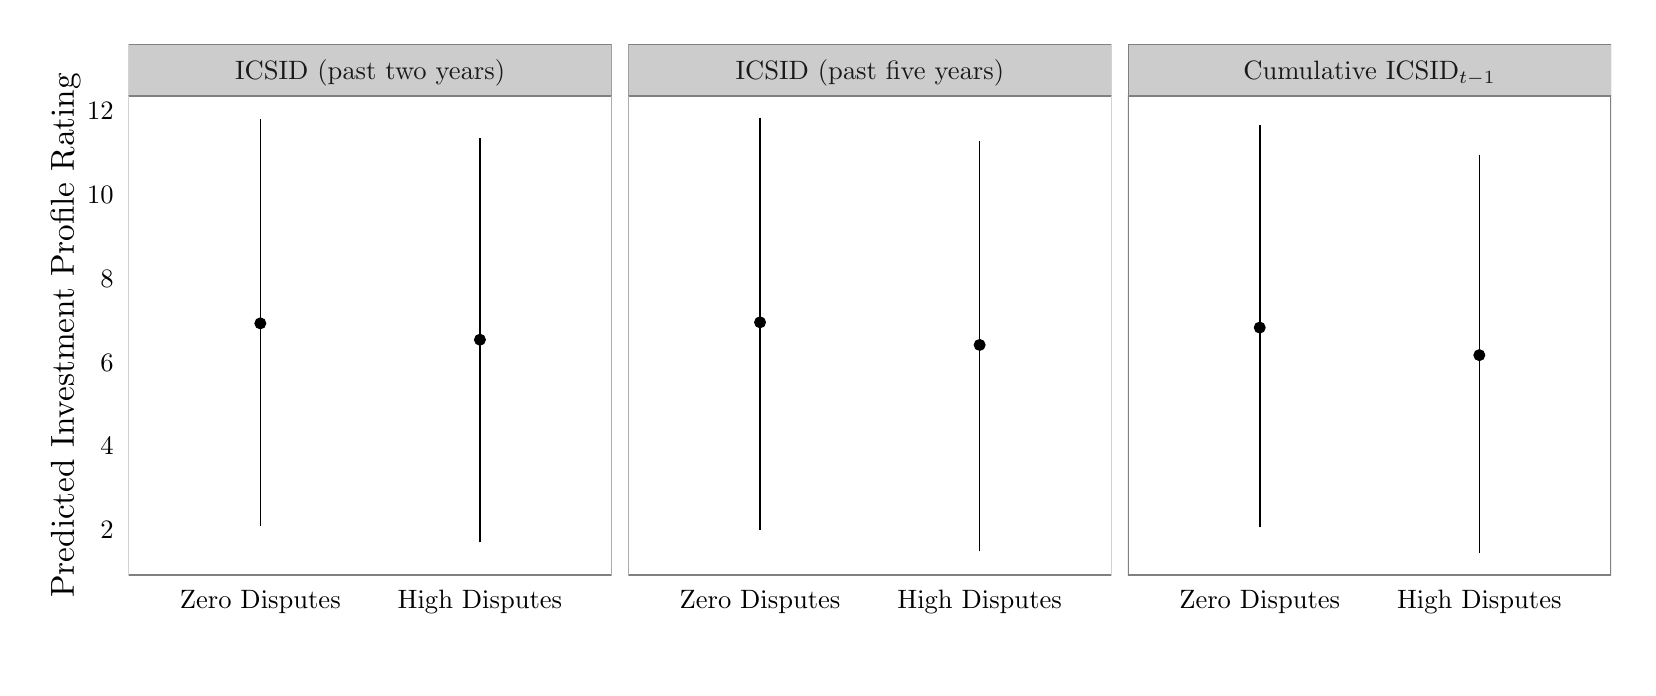
\begin{tikzpicture}[x=1pt,y=1pt]
\definecolor[named]{drawColor}{rgb}{0.00,0.00,0.00}
\definecolor[named]{fillColor}{rgb}{1.00,1.00,1.00}
\fill[color=fillColor,] (0,0) rectangle (578.16,231.26);
\begin{scope}
\path[clip] (  0.00,  0.00) rectangle (578.16,231.26);
\end{scope}
\begin{scope}
\path[clip] (  0.00,  0.00) rectangle (578.16,231.26);
\end{scope}
\begin{scope}
\path[clip] (  0.00,  0.00) rectangle (578.16,231.26);
\end{scope}
\begin{scope}
\path[clip] (  0.00,  0.00) rectangle (578.16,231.26);
\end{scope}
\begin{scope}
\path[clip] (  0.00,  0.00) rectangle (578.16,231.26);
\end{scope}
\begin{scope}
\path[clip] (  0.00,  0.00) rectangle (578.16,231.26);
\end{scope}
\begin{scope}
\path[clip] (  0.00,  0.00) rectangle (578.16,231.26);
\end{scope}
\begin{scope}
\path[clip] (  0.00,  0.00) rectangle (578.16,231.26);
\end{scope}
\begin{scope}
\path[clip] (  0.00,  0.00) rectangle (578.16,231.26);
\end{scope}
\begin{scope}
\path[clip] (  0.00,  0.00) rectangle (578.16,231.26);
\end{scope}
\begin{scope}
\path[clip] (  0.00,  0.00) rectangle (578.16,231.26);
\end{scope}
\begin{scope}
\path[clip] (  0.00,  0.00) rectangle (578.16,231.26);
\end{scope}
\begin{scope}
\path[clip] (  0.00,  0.00) rectangle (578.16,231.26);
\end{scope}
\begin{scope}
\path[clip] (  0.00,  0.00) rectangle (578.16,231.26);
\definecolor[named]{drawColor}{rgb}{1.00,1.00,1.00}
\definecolor[named]{fillColor}{rgb}{1.00,1.00,1.00}

\draw[color=drawColor,line width= 0.6pt,line cap=round,line join=round,fill=fillColor,] (  0.00,  0.00) rectangle (578.16,231.26);
\end{scope}
\begin{scope}
\path[clip] (  0.00,  0.00) rectangle (578.16,231.26);
\end{scope}
\begin{scope}
\path[clip] ( 36.46, 33.48) rectangle (211.03,206.65);
\definecolor[named]{fillColor}{rgb}{1.00,1.00,1.00}

\draw[fill=fillColor,draw opacity=0.00,] ( 36.46, 33.48) rectangle (211.03,206.65);
\definecolor[named]{drawColor}{rgb}{0.00,0.00,0.00}
\definecolor[named]{fillColor}{rgb}{0.00,0.00,0.00}

\draw[color=drawColor,line width= 0.6pt,line join=round,fill=fillColor,] ( 84.07, 51.23) -- ( 84.07,198.22);

\draw[color=drawColor,line width= 0.6pt,line join=round,fill=fillColor,] (163.42, 45.31) -- (163.42,191.56);

\draw[color=drawColor,line width= 0.4pt,line cap=round,line join=round,fill=fillColor,] ( 84.07,124.41) circle (  1.96);

\draw[color=drawColor,line width= 0.4pt,line cap=round,line join=round,fill=fillColor,] (163.42,118.50) circle (  1.96);
\definecolor[named]{drawColor}{rgb}{0.50,0.50,0.50}

\draw[color=drawColor,line width= 0.6pt,line cap=round,line join=round,fill opacity=0.00,] ( 36.46, 33.48) rectangle (211.03,206.65);
\end{scope}
\begin{scope}
\path[clip] (  0.00,  0.00) rectangle (578.16,231.26);
\end{scope}
\begin{scope}
\path[clip] (217.03, 33.48) rectangle (391.59,206.65);
\definecolor[named]{fillColor}{rgb}{1.00,1.00,1.00}

\draw[fill=fillColor,draw opacity=0.00,] (217.03, 33.48) rectangle (391.59,206.65);
\definecolor[named]{drawColor}{rgb}{0.00,0.00,0.00}
\definecolor[named]{fillColor}{rgb}{0.00,0.00,0.00}

\draw[color=drawColor,line width= 0.6pt,line join=round,fill=fillColor,] (264.64, 49.75) -- (264.64,198.78);

\draw[color=drawColor,line width= 0.6pt,line join=round,fill=fillColor,] (343.99, 42.06) -- (343.99,190.16);

\draw[color=drawColor,line width= 0.4pt,line cap=round,line join=round,fill=fillColor,] (264.64,124.79) circle (  1.96);

\draw[color=drawColor,line width= 0.4pt,line cap=round,line join=round,fill=fillColor,] (343.99,116.61) circle (  1.96);
\definecolor[named]{drawColor}{rgb}{0.50,0.50,0.50}

\draw[color=drawColor,line width= 0.6pt,line cap=round,line join=round,fill opacity=0.00,] (217.03, 33.48) rectangle (391.59,206.65);
\end{scope}
\begin{scope}
\path[clip] (  0.00,  0.00) rectangle (578.16,231.26);
\end{scope}
\begin{scope}
\path[clip] (397.59, 33.48) rectangle (572.16,206.65);
\definecolor[named]{fillColor}{rgb}{1.00,1.00,1.00}

\draw[fill=fillColor,draw opacity=0.00,] (397.59, 33.48) rectangle (572.16,206.65);
\definecolor[named]{drawColor}{rgb}{0.00,0.00,0.00}
\definecolor[named]{fillColor}{rgb}{0.00,0.00,0.00}

\draw[color=drawColor,line width= 0.6pt,line join=round,fill=fillColor,] (445.20, 50.70) -- (445.20,196.03);

\draw[color=drawColor,line width= 0.6pt,line join=round,fill=fillColor,] (524.55, 41.35) -- (524.55,185.34);

\draw[color=drawColor,line width= 0.4pt,line cap=round,line join=round,fill=fillColor,] (445.20,122.89) circle (  1.96);

\draw[color=drawColor,line width= 0.4pt,line cap=round,line join=round,fill=fillColor,] (524.55,112.93) circle (  1.96);
\definecolor[named]{drawColor}{rgb}{0.50,0.50,0.50}

\draw[color=drawColor,line width= 0.6pt,line cap=round,line join=round,fill opacity=0.00,] (397.59, 33.48) rectangle (572.16,206.65);
\end{scope}
\begin{scope}
\path[clip] (  0.00,  0.00) rectangle (578.16,231.26);
\end{scope}
\begin{scope}
\path[clip] (  0.00,  0.00) rectangle (578.16,231.26);
\end{scope}
\begin{scope}
\path[clip] (  0.00,  0.00) rectangle (578.16,231.26);
\end{scope}
\begin{scope}
\path[clip] ( 36.46,206.65) rectangle (211.03,225.26);
\definecolor[named]{drawColor}{rgb}{0.50,0.50,0.50}
\definecolor[named]{fillColor}{rgb}{0.80,0.80,0.80}

\draw[color=drawColor,line width= 0.2pt,line cap=round,line join=round,fill=fillColor,] ( 36.46,206.65) rectangle (211.03,225.26);
\definecolor[named]{drawColor}{rgb}{0.10,0.10,0.10}

\node[color=drawColor,anchor=base,inner sep=0pt, outer sep=0pt, scale=  0.96] at (123.75,212.65) {ICSID (past two years)%
};
\end{scope}
\begin{scope}
\path[clip] ( 36.46,206.65) rectangle (211.03,225.26);
\end{scope}
\begin{scope}
\path[clip] (  0.00,  0.00) rectangle (578.16,231.26);
\end{scope}
\begin{scope}
\path[clip] (  0.00,  0.00) rectangle (578.16,231.26);
\end{scope}
\begin{scope}
\path[clip] (  0.00,  0.00) rectangle (578.16,231.26);
\end{scope}
\begin{scope}
\path[clip] (  0.00,  0.00) rectangle (578.16,231.26);
\end{scope}
\begin{scope}
\path[clip] (  0.00,  0.00) rectangle (578.16,231.26);
\end{scope}
\begin{scope}
\path[clip] (  0.00,  0.00) rectangle (578.16,231.26);
\end{scope}
\begin{scope}
\path[clip] (217.03,206.65) rectangle (391.59,225.26);
\definecolor[named]{drawColor}{rgb}{0.50,0.50,0.50}
\definecolor[named]{fillColor}{rgb}{0.80,0.80,0.80}

\draw[color=drawColor,line width= 0.2pt,line cap=round,line join=round,fill=fillColor,] (217.03,206.65) rectangle (391.59,225.26);
\definecolor[named]{drawColor}{rgb}{0.10,0.10,0.10}

\node[color=drawColor,anchor=base,inner sep=0pt, outer sep=0pt, scale=  0.96] at (304.31,212.65) {ICSID (past five years)%
};
\end{scope}
\begin{scope}
\path[clip] (217.03,206.65) rectangle (391.59,225.26);
\end{scope}
\begin{scope}
\path[clip] (  0.00,  0.00) rectangle (578.16,231.26);
\end{scope}
\begin{scope}
\path[clip] (  0.00,  0.00) rectangle (578.16,231.26);
\end{scope}
\begin{scope}
\path[clip] (  0.00,  0.00) rectangle (578.16,231.26);
\end{scope}
\begin{scope}
\path[clip] (  0.00,  0.00) rectangle (578.16,231.26);
\end{scope}
\begin{scope}
\path[clip] (  0.00,  0.00) rectangle (578.16,231.26);
\end{scope}
\begin{scope}
\path[clip] (  0.00,  0.00) rectangle (578.16,231.26);
\end{scope}
\begin{scope}
\path[clip] (397.59,206.65) rectangle (572.16,225.26);
\definecolor[named]{drawColor}{rgb}{0.50,0.50,0.50}
\definecolor[named]{fillColor}{rgb}{0.80,0.80,0.80}

\draw[color=drawColor,line width= 0.2pt,line cap=round,line join=round,fill=fillColor,] (397.59,206.65) rectangle (572.16,225.26);
\definecolor[named]{drawColor}{rgb}{0.10,0.10,0.10}

\node[color=drawColor,anchor=base,inner sep=0pt, outer sep=0pt, scale=  0.96] at (484.88,212.65) {Cumulative ICSID$_{t-1}$%
};
\end{scope}
\begin{scope}
\path[clip] (397.59,206.65) rectangle (572.16,225.26);
\end{scope}
\begin{scope}
\path[clip] (  0.00,  0.00) rectangle (578.16,231.26);
\end{scope}
\begin{scope}
\path[clip] (  0.00,  0.00) rectangle (578.16,231.26);
\end{scope}
\begin{scope}
\path[clip] (  0.00,  0.00) rectangle (578.16,231.26);
\end{scope}
\begin{scope}
\path[clip] (  0.00,  0.00) rectangle (578.16,231.26);
\end{scope}
\begin{scope}
\path[clip] (  0.00,  0.00) rectangle (578.16,231.26);
\end{scope}
\begin{scope}
\path[clip] (  0.00,  0.00) rectangle (578.16,231.26);
\end{scope}
\begin{scope}
\path[clip] (  0.00,  0.00) rectangle (578.16,231.26);
\end{scope}
\begin{scope}
\path[clip] (  0.00,  0.00) rectangle (578.16,231.26);
\end{scope}
\begin{scope}
\path[clip] (  0.00,  0.00) rectangle (578.16,231.26);
\definecolor[named]{drawColor}{rgb}{0.00,0.00,0.00}

\node[color=drawColor,anchor=base east,inner sep=0pt, outer sep=0pt, scale=  0.96] at ( 31.06, 46.57) {2%
};

\node[color=drawColor,anchor=base east,inner sep=0pt, outer sep=0pt, scale=  0.96] at ( 31.06, 76.85) {4%
};

\node[color=drawColor,anchor=base east,inner sep=0pt, outer sep=0pt, scale=  0.96] at ( 31.06,107.14) {6%
};

\node[color=drawColor,anchor=base east,inner sep=0pt, outer sep=0pt, scale=  0.96] at ( 31.06,137.42) {8%
};

\node[color=drawColor,anchor=base east,inner sep=0pt, outer sep=0pt, scale=  0.96] at ( 31.06,167.70) {10%
};

\node[color=drawColor,anchor=base east,inner sep=0pt, outer sep=0pt, scale=  0.96] at ( 31.06,197.98) {12%
};
\end{scope}
\begin{scope}
\path[clip] (  0.00,  0.00) rectangle (578.16,231.26);
\end{scope}
\begin{scope}
\path[clip] (  0.00,  0.00) rectangle (578.16,231.26);
\end{scope}
\begin{scope}
\path[clip] (  0.00,  0.00) rectangle (578.16,231.26);
\end{scope}
\begin{scope}
\path[clip] (  0.00,  0.00) rectangle (578.16,231.26);
\end{scope}
\begin{scope}
\path[clip] (  0.00,  0.00) rectangle (578.16,231.26);
\end{scope}
\begin{scope}
\path[clip] (  0.00,  0.00) rectangle (578.16,231.26);
\end{scope}
\begin{scope}
\path[clip] (  0.00,  0.00) rectangle (578.16,231.26);
\end{scope}
\begin{scope}
\path[clip] (  0.00,  0.00) rectangle (578.16,231.26);
\end{scope}
\begin{scope}
\path[clip] (  0.00,  0.00) rectangle (578.16,231.26);
\end{scope}
\begin{scope}
\path[clip] (  0.00,  0.00) rectangle (578.16,231.26);
\end{scope}
\begin{scope}
\path[clip] (  0.00,  0.00) rectangle (578.16,231.26);
\end{scope}
\begin{scope}
\path[clip] (  0.00,  0.00) rectangle (578.16,231.26);
\end{scope}
\begin{scope}
\path[clip] (  0.00,  0.00) rectangle (578.16,231.26);
\end{scope}
\begin{scope}
\path[clip] (  0.00,  0.00) rectangle (578.16,231.26);
\end{scope}
\begin{scope}
\path[clip] (  0.00,  0.00) rectangle (578.16,231.26);
\end{scope}
\begin{scope}
\path[clip] (  0.00,  0.00) rectangle (578.16,231.26);
\end{scope}
\begin{scope}
\path[clip] (  0.00,  0.00) rectangle (578.16,231.26);
\end{scope}
\begin{scope}
\path[clip] (  0.00,  0.00) rectangle (578.16,231.26);
\definecolor[named]{drawColor}{rgb}{0.00,0.00,0.00}

\node[color=drawColor,anchor=base,inner sep=0pt, outer sep=0pt, scale=  0.96] at ( 84.07, 21.46) {Zero Disputes%
};

\node[color=drawColor,anchor=base,inner sep=0pt, outer sep=0pt, scale=  0.96] at (163.42, 21.46) {High Disputes%
};
\end{scope}
\begin{scope}
\path[clip] (  0.00,  0.00) rectangle (578.16,231.26);
\end{scope}
\begin{scope}
\path[clip] (  0.00,  0.00) rectangle (578.16,231.26);
\end{scope}
\begin{scope}
\path[clip] (  0.00,  0.00) rectangle (578.16,231.26);
\end{scope}
\begin{scope}
\path[clip] (  0.00,  0.00) rectangle (578.16,231.26);
\end{scope}
\begin{scope}
\path[clip] (  0.00,  0.00) rectangle (578.16,231.26);
\end{scope}
\begin{scope}
\path[clip] (  0.00,  0.00) rectangle (578.16,231.26);
\end{scope}
\begin{scope}
\path[clip] (  0.00,  0.00) rectangle (578.16,231.26);
\end{scope}
\begin{scope}
\path[clip] (  0.00,  0.00) rectangle (578.16,231.26);
\end{scope}
\begin{scope}
\path[clip] (  0.00,  0.00) rectangle (578.16,231.26);
\end{scope}
\begin{scope}
\path[clip] (  0.00,  0.00) rectangle (578.16,231.26);
\end{scope}
\begin{scope}
\path[clip] (  0.00,  0.00) rectangle (578.16,231.26);
\end{scope}
\begin{scope}
\path[clip] (  0.00,  0.00) rectangle (578.16,231.26);
\definecolor[named]{drawColor}{rgb}{0.00,0.00,0.00}

\node[color=drawColor,anchor=base,inner sep=0pt, outer sep=0pt, scale=  0.96] at (264.64, 21.46) {Zero Disputes%
};

\node[color=drawColor,anchor=base,inner sep=0pt, outer sep=0pt, scale=  0.96] at (343.99, 21.46) {High Disputes%
};
\end{scope}
\begin{scope}
\path[clip] (  0.00,  0.00) rectangle (578.16,231.26);
\end{scope}
\begin{scope}
\path[clip] (  0.00,  0.00) rectangle (578.16,231.26);
\end{scope}
\begin{scope}
\path[clip] (  0.00,  0.00) rectangle (578.16,231.26);
\end{scope}
\begin{scope}
\path[clip] (  0.00,  0.00) rectangle (578.16,231.26);
\end{scope}
\begin{scope}
\path[clip] (  0.00,  0.00) rectangle (578.16,231.26);
\end{scope}
\begin{scope}
\path[clip] (  0.00,  0.00) rectangle (578.16,231.26);
\end{scope}
\begin{scope}
\path[clip] (  0.00,  0.00) rectangle (578.16,231.26);
\end{scope}
\begin{scope}
\path[clip] (  0.00,  0.00) rectangle (578.16,231.26);
\end{scope}
\begin{scope}
\path[clip] (  0.00,  0.00) rectangle (578.16,231.26);
\end{scope}
\begin{scope}
\path[clip] (  0.00,  0.00) rectangle (578.16,231.26);
\end{scope}
\begin{scope}
\path[clip] (  0.00,  0.00) rectangle (578.16,231.26);
\end{scope}
\begin{scope}
\path[clip] (  0.00,  0.00) rectangle (578.16,231.26);
\definecolor[named]{drawColor}{rgb}{0.00,0.00,0.00}

\node[color=drawColor,anchor=base,inner sep=0pt, outer sep=0pt, scale=  0.96] at (445.20, 21.46) {Zero Disputes%
};

\node[color=drawColor,anchor=base,inner sep=0pt, outer sep=0pt, scale=  0.96] at (524.55, 21.46) {High Disputes%
};
\end{scope}
\begin{scope}
\path[clip] (  0.00,  0.00) rectangle (578.16,231.26);
\end{scope}
\begin{scope}
\path[clip] (  0.00,  0.00) rectangle (578.16,231.26);
\end{scope}
\begin{scope}
\path[clip] (  0.00,  0.00) rectangle (578.16,231.26);
\end{scope}
\begin{scope}
\path[clip] (  0.00,  0.00) rectangle (578.16,231.26);
\end{scope}
\begin{scope}
\path[clip] (  0.00,  0.00) rectangle (578.16,231.26);
\end{scope}
\begin{scope}
\path[clip] (  0.00,  0.00) rectangle (578.16,231.26);
\end{scope}
\begin{scope}
\path[clip] (  0.00,  0.00) rectangle (578.16,231.26);
\end{scope}
\begin{scope}
\path[clip] (  0.00,  0.00) rectangle (578.16,231.26);
\end{scope}
\begin{scope}
\path[clip] (  0.00,  0.00) rectangle (578.16,231.26);
\definecolor[named]{drawColor}{rgb}{0.00,0.00,0.00}

\node[rotate= 90.00,color=drawColor,anchor=base,inner sep=0pt, outer sep=0pt, scale=  1.20] at ( 16.66,120.06) {Predicted Investment Profile Rating%
};
\end{scope}
\begin{scope}
\path[clip] (  0.00,  0.00) rectangle (578.16,231.26);
\end{scope}
\begin{scope}
\path[clip] (  0.00,  0.00) rectangle (578.16,231.26);
\end{scope}
\begin{scope}
\path[clip] (  0.00,  0.00) rectangle (578.16,231.26);
\end{scope}
\begin{scope}
\path[clip] (  0.00,  0.00) rectangle (578.16,231.26);
\end{scope}
\begin{scope}
\path[clip] (  0.00,  0.00) rectangle (578.16,231.26);
\end{scope}
\end{tikzpicture}
}
	\caption*{Note: Here we show a typical country's predicted rating on investment profile under a scenario where a country faces a minimum versus the 99th percentile number of disputes, for each of the dispute variables this is equal to 3. Results were obtained by using simulations that accounted for inferential uncertainty. The point estimates here represent the mean predicted ratings and the line represents the 95\% level of uncertainty associated with these estimates.}
\end{figure}
\FloatBarrier

% \newpage

The fact that the level of uncertainty around our predicted values is so high, however, raises an interesting question. As we discussed earlier, the assumption that international institutions automatically generate adverse effects with regards to country reputation is questionable. Developing a system of effective enforcement is likely to take time as is reputational change. Much of the literature on investment treaties, however, assumes that dispute involvement entails predcitable costs, regardless of time period. This is an unnecessary assumption that we examine more closely by unpacking potential temporal variation in the effect that ICSID disputes have on a country's reputation.

To explore this issue, we rerun the analysis shown in Table \ref{tab:dispRepLevel} on a series of yearly level pooled models for the 1995--2011 period.\footnote{We begin our period for analysis here at 1995 because the infrequency of disputes before that date leads to cases in which no country had a dispute within the last two years.} All the control variables included in Table \ref{tab:dispRepLevel} are used here as well. Since our substantive interest is in how the effect of disputes has changed over time, for the sake of space we only show the coefficient results for our dispute measures in Figure \ref{fig:dispEffectYear}. The dot in each line represents the coefficient estimate for a disputes variable in a given year, with the line width representing the 95 percent confidence interval around that point estimate. Coefficient estimates that are significant at a 95 percent confidence interval are colored in black. 

\begin{figure}[ht]
	\vspace{4cm}
	\centering
	\caption{Change in Effect of Disputes Over Time}
	\label{fig:dispEffectYear}
	\resizebox{1\textwidth}{!}{% Created by tikzDevice version 0.7.0 on 2015-01-23 00:08:45
% !TEX encoding = UTF-8 Unicode
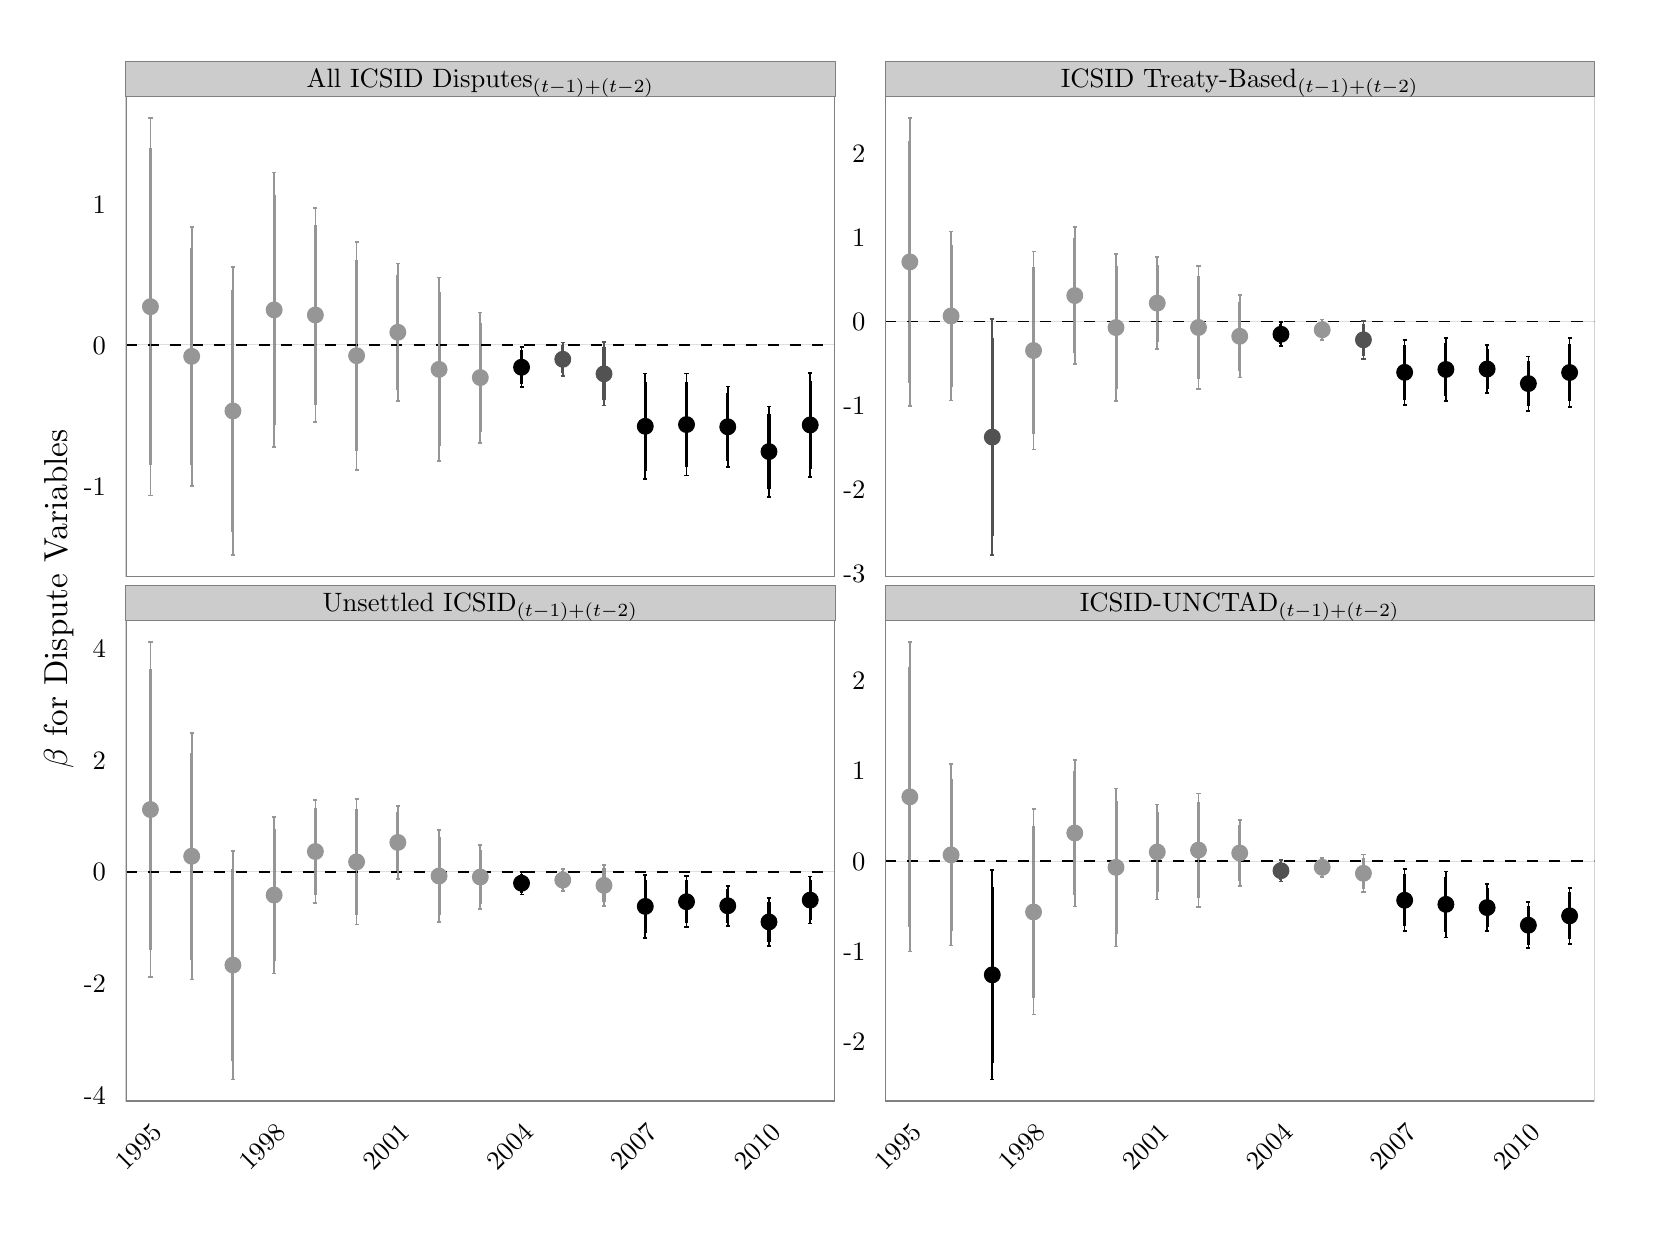
\begin{tikzpicture}[x=1pt,y=1pt]
\definecolor[named]{fillColor}{rgb}{1.00,1.00,1.00}
\path[use as bounding box,fill=fillColor,fill opacity=0.00] (0,0) rectangle (578.16,433.62);
\begin{scope}
\path[clip] (  0.00,  0.00) rectangle (578.16,433.62);
\definecolor[named]{drawColor}{rgb}{1.00,1.00,1.00}
\definecolor[named]{fillColor}{rgb}{1.00,1.00,1.00}

\path[draw=drawColor,line width= 0.6pt,line join=round,line cap=round,fill=fillColor] (  0.00,  0.00) rectangle (578.16,433.62);
\end{scope}
\begin{scope}
\path[clip] ( 35.42,235.13) rectangle (291.71,408.94);
\definecolor[named]{fillColor}{rgb}{1.00,1.00,1.00}

\path[fill=fillColor] ( 35.42,235.13) rectangle (291.71,408.94);
\definecolor[named]{drawColor}{rgb}{0.59,0.59,0.59}
\definecolor[named]{fillColor}{rgb}{0.59,0.59,0.59}

\path[draw=drawColor,draw opacity=0.30,line width= 0.3pt,line join=round,fill=fillColor,fill opacity=0.30] ( 44.36,264.57) -- ( 44.36,401.04);

\path[draw=drawColor,draw opacity=0.30,line width= 0.3pt,line join=round,fill=fillColor,fill opacity=0.30] ( 59.26,268.08) -- ( 59.26,361.64);

\path[draw=drawColor,draw opacity=0.30,line width= 0.3pt,line join=round,fill=fillColor,fill opacity=0.30] ( 74.16,243.03) -- ( 74.16,347.20);

\path[draw=drawColor,draw opacity=0.30,line width= 0.3pt,line join=round,fill=fillColor,fill opacity=0.30] ( 89.06,282.03) -- ( 89.06,381.24);

\path[draw=drawColor,draw opacity=0.30,line width= 0.3pt,line join=round,fill=fillColor,fill opacity=0.30] (103.96,291.12) -- (103.96,368.46);

\path[draw=drawColor,draw opacity=0.30,line width= 0.3pt,line join=round,fill=fillColor,fill opacity=0.30] (118.86,273.90) -- (118.86,356.28);

\path[draw=drawColor,draw opacity=0.30,line width= 0.3pt,line join=round,fill=fillColor,fill opacity=0.30] (133.76,298.70) -- (133.76,348.40);

\path[draw=drawColor,draw opacity=0.30,line width= 0.3pt,line join=round,fill=fillColor,fill opacity=0.30] (148.66,276.98) -- (148.66,343.29);

\path[draw=drawColor,draw opacity=0.30,line width= 0.3pt,line join=round,fill=fillColor,fill opacity=0.30] (163.56,283.63) -- (163.56,330.74);
\definecolor[named]{drawColor}{rgb}{0.00,0.00,0.00}
\definecolor[named]{fillColor}{rgb}{0.00,0.00,0.00}

\path[draw=drawColor,draw opacity=0.30,line width= 0.3pt,line join=round,fill=fillColor,fill opacity=0.30] (178.46,303.67) -- (178.46,318.14);
\definecolor[named]{drawColor}{rgb}{0.32,0.32,0.32}
\definecolor[named]{fillColor}{rgb}{0.32,0.32,0.32}

\path[draw=drawColor,draw opacity=0.30,line width= 0.3pt,line join=round,fill=fillColor,fill opacity=0.30] (193.36,307.68) -- (193.36,319.90);

\path[draw=drawColor,draw opacity=0.30,line width= 0.3pt,line join=round,fill=fillColor,fill opacity=0.30] (208.26,297.13) -- (208.26,319.93);
\definecolor[named]{drawColor}{rgb}{0.00,0.00,0.00}
\definecolor[named]{fillColor}{rgb}{0.00,0.00,0.00}

\path[draw=drawColor,draw opacity=0.30,line width= 0.3pt,line join=round,fill=fillColor,fill opacity=0.30] (223.17,270.42) -- (223.17,308.71);

\path[draw=drawColor,draw opacity=0.30,line width= 0.3pt,line join=round,fill=fillColor,fill opacity=0.30] (238.07,271.74) -- (238.07,308.67);

\path[draw=drawColor,draw opacity=0.30,line width= 0.3pt,line join=round,fill=fillColor,fill opacity=0.30] (252.97,274.84) -- (252.97,303.93);

\path[draw=drawColor,draw opacity=0.30,line width= 0.3pt,line join=round,fill=fillColor,fill opacity=0.30] (267.87,264.12) -- (267.87,296.74);

\path[draw=drawColor,draw opacity=0.30,line width= 0.3pt,line join=round,fill=fillColor,fill opacity=0.30] (282.77,271.21) -- (282.77,308.92);
\definecolor[named]{drawColor}{rgb}{0.59,0.59,0.59}
\definecolor[named]{fillColor}{rgb}{0.59,0.59,0.59}

\path[draw=drawColor,line width= 1.1pt,line join=round,fill=fillColor] ( 44.36,275.54) -- ( 44.36,390.07);

\path[draw=drawColor,line width= 1.1pt,line join=round,fill=fillColor] ( 59.26,275.60) -- ( 59.26,354.12);

\path[draw=drawColor,line width= 1.1pt,line join=round,fill=fillColor] ( 74.16,251.40) -- ( 74.16,338.82);

\path[draw=drawColor,line width= 1.1pt,line join=round,fill=fillColor] ( 89.06,290.00) -- ( 89.06,373.26);

\path[draw=drawColor,line width= 1.1pt,line join=round,fill=fillColor] (103.96,297.34) -- (103.96,362.24);

\path[draw=drawColor,line width= 1.1pt,line join=round,fill=fillColor] (118.86,280.52) -- (118.86,349.65);

\path[draw=drawColor,line width= 1.1pt,line join=round,fill=fillColor] (133.76,302.70) -- (133.76,344.41);

\path[draw=drawColor,line width= 1.1pt,line join=round,fill=fillColor] (148.66,282.31) -- (148.66,337.96);

\path[draw=drawColor,line width= 1.1pt,line join=round,fill=fillColor] (163.56,287.42) -- (163.56,326.95);
\definecolor[named]{drawColor}{rgb}{0.00,0.00,0.00}
\definecolor[named]{fillColor}{rgb}{0.00,0.00,0.00}

\path[draw=drawColor,line width= 1.1pt,line join=round,fill=fillColor] (178.46,304.83) -- (178.46,316.98);
\definecolor[named]{drawColor}{rgb}{0.32,0.32,0.32}
\definecolor[named]{fillColor}{rgb}{0.32,0.32,0.32}

\path[draw=drawColor,line width= 1.1pt,line join=round,fill=fillColor] (193.36,308.66) -- (193.36,318.92);

\path[draw=drawColor,line width= 1.1pt,line join=round,fill=fillColor] (208.26,298.97) -- (208.26,318.10);
\definecolor[named]{drawColor}{rgb}{0.00,0.00,0.00}
\definecolor[named]{fillColor}{rgb}{0.00,0.00,0.00}

\path[draw=drawColor,line width= 1.1pt,line join=round,fill=fillColor] (223.17,273.50) -- (223.17,305.63);

\path[draw=drawColor,line width= 1.1pt,line join=round,fill=fillColor] (238.07,274.71) -- (238.07,305.70);

\path[draw=drawColor,line width= 1.1pt,line join=round,fill=fillColor] (252.97,277.18) -- (252.97,301.59);

\path[draw=drawColor,line width= 1.1pt,line join=round,fill=fillColor] (267.87,266.74) -- (267.87,294.12);

\path[draw=drawColor,line width= 1.1pt,line join=round,fill=fillColor] (282.77,274.24) -- (282.77,305.89);

\path[draw=drawColor,line width= 0.6pt,dash pattern=on 4pt off 4pt ,line join=round,fill=fillColor] ( 35.42,318.97) -- (291.71,318.97);
\definecolor[named]{drawColor}{rgb}{0.59,0.59,0.59}
\definecolor[named]{fillColor}{rgb}{0.59,0.59,0.59}

\path[draw=drawColor,line width= 0.4pt,line join=round,line cap=round,fill=fillColor] ( 44.36,332.80) circle (  2.85);

\path[draw=drawColor,line width= 0.4pt,line join=round,line cap=round,fill=fillColor] ( 59.26,314.86) circle (  2.85);

\path[draw=drawColor,line width= 0.4pt,line join=round,line cap=round,fill=fillColor] ( 74.16,295.11) circle (  2.85);

\path[draw=drawColor,line width= 0.4pt,line join=round,line cap=round,fill=fillColor] ( 89.06,331.63) circle (  2.85);

\path[draw=drawColor,line width= 0.4pt,line join=round,line cap=round,fill=fillColor] (103.96,329.79) circle (  2.85);

\path[draw=drawColor,line width= 0.4pt,line join=round,line cap=round,fill=fillColor] (118.86,315.09) circle (  2.85);

\path[draw=drawColor,line width= 0.4pt,line join=round,line cap=round,fill=fillColor] (133.76,323.55) circle (  2.85);

\path[draw=drawColor,line width= 0.4pt,line join=round,line cap=round,fill=fillColor] (148.66,310.14) circle (  2.85);

\path[draw=drawColor,line width= 0.4pt,line join=round,line cap=round,fill=fillColor] (163.56,307.18) circle (  2.85);
\definecolor[named]{drawColor}{rgb}{0.00,0.00,0.00}
\definecolor[named]{fillColor}{rgb}{0.00,0.00,0.00}

\path[draw=drawColor,line width= 0.4pt,line join=round,line cap=round,fill=fillColor] (178.46,310.91) circle (  2.85);
\definecolor[named]{drawColor}{rgb}{0.32,0.32,0.32}
\definecolor[named]{fillColor}{rgb}{0.32,0.32,0.32}

\path[draw=drawColor,line width= 0.4pt,line join=round,line cap=round,fill=fillColor] (193.36,313.79) circle (  2.85);

\path[draw=drawColor,line width= 0.4pt,line join=round,line cap=round,fill=fillColor] (208.26,308.53) circle (  2.85);
\definecolor[named]{drawColor}{rgb}{0.00,0.00,0.00}
\definecolor[named]{fillColor}{rgb}{0.00,0.00,0.00}

\path[draw=drawColor,line width= 0.4pt,line join=round,line cap=round,fill=fillColor] (223.17,289.57) circle (  2.85);

\path[draw=drawColor,line width= 0.4pt,line join=round,line cap=round,fill=fillColor] (238.07,290.20) circle (  2.85);

\path[draw=drawColor,line width= 0.4pt,line join=round,line cap=round,fill=fillColor] (252.97,289.39) circle (  2.85);

\path[draw=drawColor,line width= 0.4pt,line join=round,line cap=round,fill=fillColor] (267.87,280.43) circle (  2.85);

\path[draw=drawColor,line width= 0.4pt,line join=round,line cap=round,fill=fillColor] (282.77,290.06) circle (  2.85);
\definecolor[named]{drawColor}{rgb}{0.59,0.59,0.59}

\path[draw=drawColor,line width= 0.6pt,line join=round] ( 43.62,401.04) --
	( 45.11,401.04);

\path[draw=drawColor,line width= 0.6pt,line join=round] ( 44.36,401.04) --
	( 44.36,264.57);

\path[draw=drawColor,line width= 0.6pt,line join=round] ( 43.62,264.57) --
	( 45.11,264.57);

\path[draw=drawColor,line width= 0.6pt,line join=round] ( 58.52,361.64) --
	( 60.01,361.64);

\path[draw=drawColor,line width= 0.6pt,line join=round] ( 59.26,361.64) --
	( 59.26,268.08);

\path[draw=drawColor,line width= 0.6pt,line join=round] ( 58.52,268.08) --
	( 60.01,268.08);

\path[draw=drawColor,line width= 0.6pt,line join=round] ( 73.42,347.20) --
	( 74.91,347.20);

\path[draw=drawColor,line width= 0.6pt,line join=round] ( 74.16,347.20) --
	( 74.16,243.03);

\path[draw=drawColor,line width= 0.6pt,line join=round] ( 73.42,243.03) --
	( 74.91,243.03);

\path[draw=drawColor,line width= 0.6pt,line join=round] ( 88.32,381.24) --
	( 89.81,381.24);

\path[draw=drawColor,line width= 0.6pt,line join=round] ( 89.06,381.24) --
	( 89.06,282.03);

\path[draw=drawColor,line width= 0.6pt,line join=round] ( 88.32,282.03) --
	( 89.81,282.03);

\path[draw=drawColor,line width= 0.6pt,line join=round] (103.22,368.46) --
	(104.71,368.46);

\path[draw=drawColor,line width= 0.6pt,line join=round] (103.96,368.46) --
	(103.96,291.12);

\path[draw=drawColor,line width= 0.6pt,line join=round] (103.22,291.12) --
	(104.71,291.12);

\path[draw=drawColor,line width= 0.6pt,line join=round] (118.12,356.28) --
	(119.61,356.28);

\path[draw=drawColor,line width= 0.6pt,line join=round] (118.86,356.28) --
	(118.86,273.90);

\path[draw=drawColor,line width= 0.6pt,line join=round] (118.12,273.90) --
	(119.61,273.90);

\path[draw=drawColor,line width= 0.6pt,line join=round] (133.02,348.40) --
	(134.51,348.40);

\path[draw=drawColor,line width= 0.6pt,line join=round] (133.76,348.40) --
	(133.76,298.70);

\path[draw=drawColor,line width= 0.6pt,line join=round] (133.02,298.70) --
	(134.51,298.70);

\path[draw=drawColor,line width= 0.6pt,line join=round] (147.92,343.29) --
	(149.41,343.29);

\path[draw=drawColor,line width= 0.6pt,line join=round] (148.66,343.29) --
	(148.66,276.98);

\path[draw=drawColor,line width= 0.6pt,line join=round] (147.92,276.98) --
	(149.41,276.98);

\path[draw=drawColor,line width= 0.6pt,line join=round] (162.82,330.74) --
	(164.31,330.74);

\path[draw=drawColor,line width= 0.6pt,line join=round] (163.56,330.74) --
	(163.56,283.63);

\path[draw=drawColor,line width= 0.6pt,line join=round] (162.82,283.63) --
	(164.31,283.63);
\definecolor[named]{drawColor}{rgb}{0.00,0.00,0.00}

\path[draw=drawColor,line width= 0.6pt,line join=round] (177.72,318.14) --
	(179.21,318.14);

\path[draw=drawColor,line width= 0.6pt,line join=round] (178.46,318.14) --
	(178.46,303.67);

\path[draw=drawColor,line width= 0.6pt,line join=round] (177.72,303.67) --
	(179.21,303.67);
\definecolor[named]{drawColor}{rgb}{0.32,0.32,0.32}

\path[draw=drawColor,line width= 0.6pt,line join=round] (192.62,319.90) --
	(194.11,319.90);

\path[draw=drawColor,line width= 0.6pt,line join=round] (193.36,319.90) --
	(193.36,307.68);

\path[draw=drawColor,line width= 0.6pt,line join=round] (192.62,307.68) --
	(194.11,307.68);

\path[draw=drawColor,line width= 0.6pt,line join=round] (207.52,319.93) --
	(209.01,319.93);

\path[draw=drawColor,line width= 0.6pt,line join=round] (208.26,319.93) --
	(208.26,297.13);

\path[draw=drawColor,line width= 0.6pt,line join=round] (207.52,297.13) --
	(209.01,297.13);
\definecolor[named]{drawColor}{rgb}{0.00,0.00,0.00}

\path[draw=drawColor,line width= 0.6pt,line join=round] (222.42,308.71) --
	(223.91,308.71);

\path[draw=drawColor,line width= 0.6pt,line join=round] (223.17,308.71) --
	(223.17,270.42);

\path[draw=drawColor,line width= 0.6pt,line join=round] (222.42,270.42) --
	(223.91,270.42);

\path[draw=drawColor,line width= 0.6pt,line join=round] (237.32,308.67) --
	(238.81,308.67);

\path[draw=drawColor,line width= 0.6pt,line join=round] (238.07,308.67) --
	(238.07,271.74);

\path[draw=drawColor,line width= 0.6pt,line join=round] (237.32,271.74) --
	(238.81,271.74);

\path[draw=drawColor,line width= 0.6pt,line join=round] (252.22,303.93) --
	(253.71,303.93);

\path[draw=drawColor,line width= 0.6pt,line join=round] (252.97,303.93) --
	(252.97,274.84);

\path[draw=drawColor,line width= 0.6pt,line join=round] (252.22,274.84) --
	(253.71,274.84);

\path[draw=drawColor,line width= 0.6pt,line join=round] (267.12,296.74) --
	(268.61,296.74);

\path[draw=drawColor,line width= 0.6pt,line join=round] (267.87,296.74) --
	(267.87,264.12);

\path[draw=drawColor,line width= 0.6pt,line join=round] (267.12,264.12) --
	(268.61,264.12);

\path[draw=drawColor,line width= 0.6pt,line join=round] (282.02,308.92) --
	(283.51,308.92);

\path[draw=drawColor,line width= 0.6pt,line join=round] (282.77,308.92) --
	(282.77,271.21);

\path[draw=drawColor,line width= 0.6pt,line join=round] (282.02,271.21) --
	(283.51,271.21);
\definecolor[named]{drawColor}{rgb}{0.50,0.50,0.50}

\path[draw=drawColor,line width= 0.6pt,line join=round,line cap=round] ( 35.42,235.13) rectangle (291.71,408.94);
\end{scope}
\begin{scope}
\path[clip] (309.83,235.13) rectangle (566.12,408.94);
\definecolor[named]{fillColor}{rgb}{1.00,1.00,1.00}

\path[fill=fillColor] (309.83,235.13) rectangle (566.12,408.94);
\definecolor[named]{drawColor}{rgb}{0.59,0.59,0.59}
\definecolor[named]{fillColor}{rgb}{0.59,0.59,0.59}

\path[draw=drawColor,draw opacity=0.30,line width= 0.3pt,line join=round,fill=fillColor,fill opacity=0.30] (318.77,296.91) -- (318.77,401.04);

\path[draw=drawColor,draw opacity=0.30,line width= 0.3pt,line join=round,fill=fillColor,fill opacity=0.30] (333.67,298.91) -- (333.67,359.98);
\definecolor[named]{drawColor}{rgb}{0.32,0.32,0.32}
\definecolor[named]{fillColor}{rgb}{0.32,0.32,0.32}

\path[draw=drawColor,draw opacity=0.30,line width= 0.3pt,line join=round,fill=fillColor,fill opacity=0.30] (348.57,243.03) -- (348.57,328.29);
\definecolor[named]{drawColor}{rgb}{0.59,0.59,0.59}
\definecolor[named]{fillColor}{rgb}{0.59,0.59,0.59}

\path[draw=drawColor,draw opacity=0.30,line width= 0.3pt,line join=round,fill=fillColor,fill opacity=0.30] (363.47,281.18) -- (363.47,352.72);

\path[draw=drawColor,draw opacity=0.30,line width= 0.3pt,line join=round,fill=fillColor,fill opacity=0.30] (378.37,312.13) -- (378.37,361.49);

\path[draw=drawColor,draw opacity=0.30,line width= 0.3pt,line join=round,fill=fillColor,fill opacity=0.30] (393.27,298.64) -- (393.27,351.85);

\path[draw=drawColor,draw opacity=0.30,line width= 0.3pt,line join=round,fill=fillColor,fill opacity=0.30] (408.17,317.52) -- (408.17,350.65);

\path[draw=drawColor,draw opacity=0.30,line width= 0.3pt,line join=round,fill=fillColor,fill opacity=0.30] (423.07,302.98) -- (423.07,347.58);

\path[draw=drawColor,draw opacity=0.30,line width= 0.3pt,line join=round,fill=fillColor,fill opacity=0.30] (437.97,307.17) -- (437.97,337.03);
\definecolor[named]{drawColor}{rgb}{0.00,0.00,0.00}
\definecolor[named]{fillColor}{rgb}{0.00,0.00,0.00}

\path[draw=drawColor,draw opacity=0.30,line width= 0.3pt,line join=round,fill=fillColor,fill opacity=0.30] (452.87,318.49) -- (452.87,327.17);
\definecolor[named]{drawColor}{rgb}{0.59,0.59,0.59}
\definecolor[named]{fillColor}{rgb}{0.59,0.59,0.59}

\path[draw=drawColor,draw opacity=0.30,line width= 0.3pt,line join=round,fill=fillColor,fill opacity=0.30] (467.77,320.78) -- (467.77,328.11);
\definecolor[named]{drawColor}{rgb}{0.32,0.32,0.32}
\definecolor[named]{fillColor}{rgb}{0.32,0.32,0.32}

\path[draw=drawColor,draw opacity=0.30,line width= 0.3pt,line join=round,fill=fillColor,fill opacity=0.30] (482.67,313.93) -- (482.67,327.71);
\definecolor[named]{drawColor}{rgb}{0.00,0.00,0.00}
\definecolor[named]{fillColor}{rgb}{0.00,0.00,0.00}

\path[draw=drawColor,draw opacity=0.30,line width= 0.3pt,line join=round,fill=fillColor,fill opacity=0.30] (497.57,297.29) -- (497.57,320.85);

\path[draw=drawColor,draw opacity=0.30,line width= 0.3pt,line join=round,fill=fillColor,fill opacity=0.30] (512.47,298.78) -- (512.47,321.47);

\path[draw=drawColor,draw opacity=0.30,line width= 0.3pt,line join=round,fill=fillColor,fill opacity=0.30] (527.37,301.55) -- (527.37,318.99);

\path[draw=drawColor,draw opacity=0.30,line width= 0.3pt,line join=round,fill=fillColor,fill opacity=0.30] (542.27,295.17) -- (542.27,314.84);

\path[draw=drawColor,draw opacity=0.30,line width= 0.3pt,line join=round,fill=fillColor,fill opacity=0.30] (557.17,296.64) -- (557.17,321.39);
\definecolor[named]{drawColor}{rgb}{0.59,0.59,0.59}
\definecolor[named]{fillColor}{rgb}{0.59,0.59,0.59}

\path[draw=drawColor,line width= 1.1pt,line join=round,fill=fillColor] (318.77,305.28) -- (318.77,392.67);

\path[draw=drawColor,line width= 1.1pt,line join=round,fill=fillColor] (333.67,303.82) -- (333.67,355.07);
\definecolor[named]{drawColor}{rgb}{0.32,0.32,0.32}
\definecolor[named]{fillColor}{rgb}{0.32,0.32,0.32}

\path[draw=drawColor,line width= 1.1pt,line join=round,fill=fillColor] (348.57,249.88) -- (348.57,321.43);
\definecolor[named]{drawColor}{rgb}{0.59,0.59,0.59}
\definecolor[named]{fillColor}{rgb}{0.59,0.59,0.59}

\path[draw=drawColor,line width= 1.1pt,line join=round,fill=fillColor] (363.47,286.93) -- (363.47,346.97);

\path[draw=drawColor,line width= 1.1pt,line join=round,fill=fillColor] (378.37,316.10) -- (378.37,357.52);

\path[draw=drawColor,line width= 1.1pt,line join=round,fill=fillColor] (393.27,302.92) -- (393.27,347.57);

\path[draw=drawColor,line width= 1.1pt,line join=round,fill=fillColor] (408.17,320.18) -- (408.17,347.99);

\path[draw=drawColor,line width= 1.1pt,line join=round,fill=fillColor] (423.07,306.56) -- (423.07,343.99);

\path[draw=drawColor,line width= 1.1pt,line join=round,fill=fillColor] (437.97,309.57) -- (437.97,334.63);
\definecolor[named]{drawColor}{rgb}{0.00,0.00,0.00}
\definecolor[named]{fillColor}{rgb}{0.00,0.00,0.00}

\path[draw=drawColor,line width= 1.1pt,line join=round,fill=fillColor] (452.87,319.18) -- (452.87,326.47);
\definecolor[named]{drawColor}{rgb}{0.59,0.59,0.59}
\definecolor[named]{fillColor}{rgb}{0.59,0.59,0.59}

\path[draw=drawColor,line width= 1.1pt,line join=round,fill=fillColor] (467.77,321.37) -- (467.77,327.52);
\definecolor[named]{drawColor}{rgb}{0.32,0.32,0.32}
\definecolor[named]{fillColor}{rgb}{0.32,0.32,0.32}

\path[draw=drawColor,line width= 1.1pt,line join=round,fill=fillColor] (482.67,315.04) -- (482.67,326.60);
\definecolor[named]{drawColor}{rgb}{0.00,0.00,0.00}
\definecolor[named]{fillColor}{rgb}{0.00,0.00,0.00}

\path[draw=drawColor,line width= 1.1pt,line join=round,fill=fillColor] (497.57,299.18) -- (497.57,318.95);

\path[draw=drawColor,line width= 1.1pt,line join=round,fill=fillColor] (512.47,300.60) -- (512.47,319.64);

\path[draw=drawColor,line width= 1.1pt,line join=round,fill=fillColor] (527.37,302.95) -- (527.37,317.59);

\path[draw=drawColor,line width= 1.1pt,line join=round,fill=fillColor] (542.27,296.75) -- (542.27,313.26);

\path[draw=drawColor,line width= 1.1pt,line join=round,fill=fillColor] (557.17,298.63) -- (557.17,319.40);

\path[draw=drawColor,line width= 0.6pt,dash pattern=on 4pt off 4pt ,line join=round,fill=fillColor] (309.83,327.38) -- (566.12,327.38);
\definecolor[named]{drawColor}{rgb}{0.59,0.59,0.59}
\definecolor[named]{fillColor}{rgb}{0.59,0.59,0.59}

\path[draw=drawColor,line width= 0.4pt,line join=round,line cap=round,fill=fillColor] (318.77,348.98) circle (  2.85);

\path[draw=drawColor,line width= 0.4pt,line join=round,line cap=round,fill=fillColor] (333.67,329.45) circle (  2.85);
\definecolor[named]{drawColor}{rgb}{0.32,0.32,0.32}
\definecolor[named]{fillColor}{rgb}{0.32,0.32,0.32}

\path[draw=drawColor,line width= 0.4pt,line join=round,line cap=round,fill=fillColor] (348.57,285.66) circle (  2.85);
\definecolor[named]{drawColor}{rgb}{0.59,0.59,0.59}
\definecolor[named]{fillColor}{rgb}{0.59,0.59,0.59}

\path[draw=drawColor,line width= 0.4pt,line join=round,line cap=round,fill=fillColor] (363.47,316.95) circle (  2.85);

\path[draw=drawColor,line width= 0.4pt,line join=round,line cap=round,fill=fillColor] (378.37,336.81) circle (  2.85);

\path[draw=drawColor,line width= 0.4pt,line join=round,line cap=round,fill=fillColor] (393.27,325.24) circle (  2.85);

\path[draw=drawColor,line width= 0.4pt,line join=round,line cap=round,fill=fillColor] (408.17,334.08) circle (  2.85);

\path[draw=drawColor,line width= 0.4pt,line join=round,line cap=round,fill=fillColor] (423.07,325.28) circle (  2.85);

\path[draw=drawColor,line width= 0.4pt,line join=round,line cap=round,fill=fillColor] (437.97,322.10) circle (  2.85);
\definecolor[named]{drawColor}{rgb}{0.00,0.00,0.00}
\definecolor[named]{fillColor}{rgb}{0.00,0.00,0.00}

\path[draw=drawColor,line width= 0.4pt,line join=round,line cap=round,fill=fillColor] (452.87,322.83) circle (  2.85);
\definecolor[named]{drawColor}{rgb}{0.59,0.59,0.59}
\definecolor[named]{fillColor}{rgb}{0.59,0.59,0.59}

\path[draw=drawColor,line width= 0.4pt,line join=round,line cap=round,fill=fillColor] (467.77,324.45) circle (  2.85);
\definecolor[named]{drawColor}{rgb}{0.32,0.32,0.32}
\definecolor[named]{fillColor}{rgb}{0.32,0.32,0.32}

\path[draw=drawColor,line width= 0.4pt,line join=round,line cap=round,fill=fillColor] (482.67,320.82) circle (  2.85);
\definecolor[named]{drawColor}{rgb}{0.00,0.00,0.00}
\definecolor[named]{fillColor}{rgb}{0.00,0.00,0.00}

\path[draw=drawColor,line width= 0.4pt,line join=round,line cap=round,fill=fillColor] (497.57,309.07) circle (  2.85);

\path[draw=drawColor,line width= 0.4pt,line join=round,line cap=round,fill=fillColor] (512.47,310.12) circle (  2.85);

\path[draw=drawColor,line width= 0.4pt,line join=round,line cap=round,fill=fillColor] (527.37,310.27) circle (  2.85);

\path[draw=drawColor,line width= 0.4pt,line join=round,line cap=round,fill=fillColor] (542.27,305.01) circle (  2.85);

\path[draw=drawColor,line width= 0.4pt,line join=round,line cap=round,fill=fillColor] (557.17,309.01) circle (  2.85);
\definecolor[named]{drawColor}{rgb}{0.59,0.59,0.59}

\path[draw=drawColor,line width= 0.6pt,line join=round] (318.02,401.04) --
	(319.51,401.04);

\path[draw=drawColor,line width= 0.6pt,line join=round] (318.77,401.04) --
	(318.77,296.91);

\path[draw=drawColor,line width= 0.6pt,line join=round] (318.02,296.91) --
	(319.51,296.91);

\path[draw=drawColor,line width= 0.6pt,line join=round] (332.92,359.98) --
	(334.41,359.98);

\path[draw=drawColor,line width= 0.6pt,line join=round] (333.67,359.98) --
	(333.67,298.91);

\path[draw=drawColor,line width= 0.6pt,line join=round] (332.92,298.91) --
	(334.41,298.91);
\definecolor[named]{drawColor}{rgb}{0.32,0.32,0.32}

\path[draw=drawColor,line width= 0.6pt,line join=round] (347.83,328.29) --
	(349.32,328.29);

\path[draw=drawColor,line width= 0.6pt,line join=round] (348.57,328.29) --
	(348.57,243.03);

\path[draw=drawColor,line width= 0.6pt,line join=round] (347.83,243.03) --
	(349.32,243.03);
\definecolor[named]{drawColor}{rgb}{0.59,0.59,0.59}

\path[draw=drawColor,line width= 0.6pt,line join=round] (362.73,352.72) --
	(364.22,352.72);

\path[draw=drawColor,line width= 0.6pt,line join=round] (363.47,352.72) --
	(363.47,281.18);

\path[draw=drawColor,line width= 0.6pt,line join=round] (362.73,281.18) --
	(364.22,281.18);

\path[draw=drawColor,line width= 0.6pt,line join=round] (377.63,361.49) --
	(379.12,361.49);

\path[draw=drawColor,line width= 0.6pt,line join=round] (378.37,361.49) --
	(378.37,312.13);

\path[draw=drawColor,line width= 0.6pt,line join=round] (377.63,312.13) --
	(379.12,312.13);

\path[draw=drawColor,line width= 0.6pt,line join=round] (392.53,351.85) --
	(394.02,351.85);

\path[draw=drawColor,line width= 0.6pt,line join=round] (393.27,351.85) --
	(393.27,298.64);

\path[draw=drawColor,line width= 0.6pt,line join=round] (392.53,298.64) --
	(394.02,298.64);

\path[draw=drawColor,line width= 0.6pt,line join=round] (407.43,350.65) --
	(408.92,350.65);

\path[draw=drawColor,line width= 0.6pt,line join=round] (408.17,350.65) --
	(408.17,317.52);

\path[draw=drawColor,line width= 0.6pt,line join=round] (407.43,317.52) --
	(408.92,317.52);

\path[draw=drawColor,line width= 0.6pt,line join=round] (422.33,347.58) --
	(423.82,347.58);

\path[draw=drawColor,line width= 0.6pt,line join=round] (423.07,347.58) --
	(423.07,302.98);

\path[draw=drawColor,line width= 0.6pt,line join=round] (422.33,302.98) --
	(423.82,302.98);

\path[draw=drawColor,line width= 0.6pt,line join=round] (437.23,337.03) --
	(438.72,337.03);

\path[draw=drawColor,line width= 0.6pt,line join=round] (437.97,337.03) --
	(437.97,307.17);

\path[draw=drawColor,line width= 0.6pt,line join=round] (437.23,307.17) --
	(438.72,307.17);
\definecolor[named]{drawColor}{rgb}{0.00,0.00,0.00}

\path[draw=drawColor,line width= 0.6pt,line join=round] (452.13,327.17) --
	(453.62,327.17);

\path[draw=drawColor,line width= 0.6pt,line join=round] (452.87,327.17) --
	(452.87,318.49);

\path[draw=drawColor,line width= 0.6pt,line join=round] (452.13,318.49) --
	(453.62,318.49);
\definecolor[named]{drawColor}{rgb}{0.59,0.59,0.59}

\path[draw=drawColor,line width= 0.6pt,line join=round] (467.03,328.11) --
	(468.52,328.11);

\path[draw=drawColor,line width= 0.6pt,line join=round] (467.77,328.11) --
	(467.77,320.78);

\path[draw=drawColor,line width= 0.6pt,line join=round] (467.03,320.78) --
	(468.52,320.78);
\definecolor[named]{drawColor}{rgb}{0.32,0.32,0.32}

\path[draw=drawColor,line width= 0.6pt,line join=round] (481.93,327.71) --
	(483.42,327.71);

\path[draw=drawColor,line width= 0.6pt,line join=round] (482.67,327.71) --
	(482.67,313.93);

\path[draw=drawColor,line width= 0.6pt,line join=round] (481.93,313.93) --
	(483.42,313.93);
\definecolor[named]{drawColor}{rgb}{0.00,0.00,0.00}

\path[draw=drawColor,line width= 0.6pt,line join=round] (496.83,320.85) --
	(498.32,320.85);

\path[draw=drawColor,line width= 0.6pt,line join=round] (497.57,320.85) --
	(497.57,297.29);

\path[draw=drawColor,line width= 0.6pt,line join=round] (496.83,297.29) --
	(498.32,297.29);

\path[draw=drawColor,line width= 0.6pt,line join=round] (511.73,321.47) --
	(513.22,321.47);

\path[draw=drawColor,line width= 0.6pt,line join=round] (512.47,321.47) --
	(512.47,298.78);

\path[draw=drawColor,line width= 0.6pt,line join=round] (511.73,298.78) --
	(513.22,298.78);

\path[draw=drawColor,line width= 0.6pt,line join=round] (526.63,318.99) --
	(528.12,318.99);

\path[draw=drawColor,line width= 0.6pt,line join=round] (527.37,318.99) --
	(527.37,301.55);

\path[draw=drawColor,line width= 0.6pt,line join=round] (526.63,301.55) --
	(528.12,301.55);

\path[draw=drawColor,line width= 0.6pt,line join=round] (541.53,314.84) --
	(543.02,314.84);

\path[draw=drawColor,line width= 0.6pt,line join=round] (542.27,314.84) --
	(542.27,295.17);

\path[draw=drawColor,line width= 0.6pt,line join=round] (541.53,295.17) --
	(543.02,295.17);

\path[draw=drawColor,line width= 0.6pt,line join=round] (556.43,321.39) --
	(557.92,321.39);

\path[draw=drawColor,line width= 0.6pt,line join=round] (557.17,321.39) --
	(557.17,296.64);

\path[draw=drawColor,line width= 0.6pt,line join=round] (556.43,296.64) --
	(557.92,296.64);
\definecolor[named]{drawColor}{rgb}{0.50,0.50,0.50}

\path[draw=drawColor,line width= 0.6pt,line join=round,line cap=round] (309.83,235.13) rectangle (566.12,408.94);
\end{scope}
\begin{scope}
\path[clip] ( 35.42, 45.67) rectangle (291.71,219.48);
\definecolor[named]{fillColor}{rgb}{1.00,1.00,1.00}

\path[fill=fillColor] ( 35.42, 45.67) rectangle (291.71,219.48);
\definecolor[named]{drawColor}{rgb}{0.59,0.59,0.59}
\definecolor[named]{fillColor}{rgb}{0.59,0.59,0.59}

\path[draw=drawColor,draw opacity=0.30,line width= 0.3pt,line join=round,fill=fillColor,fill opacity=0.30] ( 44.36, 90.60) -- ( 44.36,211.58);

\path[draw=drawColor,draw opacity=0.30,line width= 0.3pt,line join=round,fill=fillColor,fill opacity=0.30] ( 59.26, 89.72) -- ( 59.26,178.73);

\path[draw=drawColor,draw opacity=0.30,line width= 0.3pt,line join=round,fill=fillColor,fill opacity=0.30] ( 74.16, 53.57) -- ( 74.16,136.22);

\path[draw=drawColor,draw opacity=0.30,line width= 0.3pt,line join=round,fill=fillColor,fill opacity=0.30] ( 89.06, 91.88) -- ( 89.06,148.49);

\path[draw=drawColor,draw opacity=0.30,line width= 0.3pt,line join=round,fill=fillColor,fill opacity=0.30] (103.96,117.41) -- (103.96,154.44);

\path[draw=drawColor,draw opacity=0.30,line width= 0.3pt,line join=round,fill=fillColor,fill opacity=0.30] (118.86,109.49) -- (118.86,154.87);

\path[draw=drawColor,draw opacity=0.30,line width= 0.3pt,line join=round,fill=fillColor,fill opacity=0.30] (133.76,126.01) -- (133.76,152.40);

\path[draw=drawColor,draw opacity=0.30,line width= 0.3pt,line join=round,fill=fillColor,fill opacity=0.30] (148.66,110.37) -- (148.66,143.77);

\path[draw=drawColor,draw opacity=0.30,line width= 0.3pt,line join=round,fill=fillColor,fill opacity=0.30] (163.56,115.24) -- (163.56,138.16);
\definecolor[named]{drawColor}{rgb}{0.00,0.00,0.00}
\definecolor[named]{fillColor}{rgb}{0.00,0.00,0.00}

\path[draw=drawColor,draw opacity=0.30,line width= 0.3pt,line join=round,fill=fillColor,fill opacity=0.30] (178.46,120.38) -- (178.46,128.55);
\definecolor[named]{drawColor}{rgb}{0.59,0.59,0.59}
\definecolor[named]{fillColor}{rgb}{0.59,0.59,0.59}

\path[draw=drawColor,draw opacity=0.30,line width= 0.3pt,line join=round,fill=fillColor,fill opacity=0.30] (193.36,121.68) -- (193.36,129.55);

\path[draw=drawColor,draw opacity=0.30,line width= 0.3pt,line join=round,fill=fillColor,fill opacity=0.30] (208.26,116.35) -- (208.26,131.02);
\definecolor[named]{drawColor}{rgb}{0.00,0.00,0.00}
\definecolor[named]{fillColor}{rgb}{0.00,0.00,0.00}

\path[draw=drawColor,draw opacity=0.30,line width= 0.3pt,line join=round,fill=fillColor,fill opacity=0.30] (223.17,104.68) -- (223.17,127.50);

\path[draw=drawColor,draw opacity=0.30,line width= 0.3pt,line join=round,fill=fillColor,fill opacity=0.30] (238.07,108.53) -- (238.07,127.04);

\path[draw=drawColor,draw opacity=0.30,line width= 0.3pt,line join=round,fill=fillColor,fill opacity=0.30] (252.97,109.06) -- (252.97,123.56);

\path[draw=drawColor,draw opacity=0.30,line width= 0.3pt,line join=round,fill=fillColor,fill opacity=0.30] (267.87,101.86) -- (267.87,119.11);

\path[draw=drawColor,draw opacity=0.30,line width= 0.3pt,line join=round,fill=fillColor,fill opacity=0.30] (282.77,109.89) -- (282.77,126.85);
\definecolor[named]{drawColor}{rgb}{0.59,0.59,0.59}
\definecolor[named]{fillColor}{rgb}{0.59,0.59,0.59}

\path[draw=drawColor,line width= 1.1pt,line join=round,fill=fillColor] ( 44.36,100.33) -- ( 44.36,201.86);

\path[draw=drawColor,line width= 1.1pt,line join=round,fill=fillColor] ( 59.26, 96.87) -- ( 59.26,171.57);

\path[draw=drawColor,line width= 1.1pt,line join=round,fill=fillColor] ( 74.16, 60.22) -- ( 74.16,129.58);

\path[draw=drawColor,line width= 1.1pt,line join=round,fill=fillColor] ( 89.06, 96.43) -- ( 89.06,143.94);

\path[draw=drawColor,line width= 1.1pt,line join=round,fill=fillColor] (103.96,120.38) -- (103.96,151.47);

\path[draw=drawColor,line width= 1.1pt,line join=round,fill=fillColor] (118.86,113.14) -- (118.86,151.22);

\path[draw=drawColor,line width= 1.1pt,line join=round,fill=fillColor] (133.76,128.13) -- (133.76,150.28);

\path[draw=drawColor,line width= 1.1pt,line join=round,fill=fillColor] (148.66,113.06) -- (148.66,141.09);

\path[draw=drawColor,line width= 1.1pt,line join=round,fill=fillColor] (163.56,117.08) -- (163.56,136.32);
\definecolor[named]{drawColor}{rgb}{0.00,0.00,0.00}
\definecolor[named]{fillColor}{rgb}{0.00,0.00,0.00}

\path[draw=drawColor,line width= 1.1pt,line join=round,fill=fillColor] (178.46,121.03) -- (178.46,127.90);
\definecolor[named]{drawColor}{rgb}{0.59,0.59,0.59}
\definecolor[named]{fillColor}{rgb}{0.59,0.59,0.59}

\path[draw=drawColor,line width= 1.1pt,line join=round,fill=fillColor] (193.36,122.31) -- (193.36,128.91);

\path[draw=drawColor,line width= 1.1pt,line join=round,fill=fillColor] (208.26,117.53) -- (208.26,129.84);
\definecolor[named]{drawColor}{rgb}{0.00,0.00,0.00}
\definecolor[named]{fillColor}{rgb}{0.00,0.00,0.00}

\path[draw=drawColor,line width= 1.1pt,line join=round,fill=fillColor] (223.17,106.51) -- (223.17,125.67);

\path[draw=drawColor,line width= 1.1pt,line join=round,fill=fillColor] (238.07,110.01) -- (238.07,125.55);

\path[draw=drawColor,line width= 1.1pt,line join=round,fill=fillColor] (252.97,110.22) -- (252.97,122.39);

\path[draw=drawColor,line width= 1.1pt,line join=round,fill=fillColor] (267.87,103.25) -- (267.87,117.72);

\path[draw=drawColor,line width= 1.1pt,line join=round,fill=fillColor] (282.77,111.26) -- (282.77,125.49);

\path[draw=drawColor,line width= 0.6pt,dash pattern=on 4pt off 4pt ,line join=round,fill=fillColor] ( 35.42,128.60) -- (291.71,128.60);
\definecolor[named]{drawColor}{rgb}{0.59,0.59,0.59}
\definecolor[named]{fillColor}{rgb}{0.59,0.59,0.59}

\path[draw=drawColor,line width= 0.4pt,line join=round,line cap=round,fill=fillColor] ( 44.36,151.09) circle (  2.85);

\path[draw=drawColor,line width= 0.4pt,line join=round,line cap=round,fill=fillColor] ( 59.26,134.22) circle (  2.85);

\path[draw=drawColor,line width= 0.4pt,line join=round,line cap=round,fill=fillColor] ( 74.16, 94.90) circle (  2.85);

\path[draw=drawColor,line width= 0.4pt,line join=round,line cap=round,fill=fillColor] ( 89.06,120.19) circle (  2.85);

\path[draw=drawColor,line width= 0.4pt,line join=round,line cap=round,fill=fillColor] (103.96,135.92) circle (  2.85);

\path[draw=drawColor,line width= 0.4pt,line join=round,line cap=round,fill=fillColor] (118.86,132.18) circle (  2.85);

\path[draw=drawColor,line width= 0.4pt,line join=round,line cap=round,fill=fillColor] (133.76,139.20) circle (  2.85);

\path[draw=drawColor,line width= 0.4pt,line join=round,line cap=round,fill=fillColor] (148.66,127.07) circle (  2.85);

\path[draw=drawColor,line width= 0.4pt,line join=round,line cap=round,fill=fillColor] (163.56,126.70) circle (  2.85);
\definecolor[named]{drawColor}{rgb}{0.00,0.00,0.00}
\definecolor[named]{fillColor}{rgb}{0.00,0.00,0.00}

\path[draw=drawColor,line width= 0.4pt,line join=round,line cap=round,fill=fillColor] (178.46,124.47) circle (  2.85);
\definecolor[named]{drawColor}{rgb}{0.59,0.59,0.59}
\definecolor[named]{fillColor}{rgb}{0.59,0.59,0.59}

\path[draw=drawColor,line width= 0.4pt,line join=round,line cap=round,fill=fillColor] (193.36,125.61) circle (  2.85);

\path[draw=drawColor,line width= 0.4pt,line join=round,line cap=round,fill=fillColor] (208.26,123.69) circle (  2.85);
\definecolor[named]{drawColor}{rgb}{0.00,0.00,0.00}
\definecolor[named]{fillColor}{rgb}{0.00,0.00,0.00}

\path[draw=drawColor,line width= 0.4pt,line join=round,line cap=round,fill=fillColor] (223.17,116.09) circle (  2.85);

\path[draw=drawColor,line width= 0.4pt,line join=round,line cap=round,fill=fillColor] (238.07,117.78) circle (  2.85);

\path[draw=drawColor,line width= 0.4pt,line join=round,line cap=round,fill=fillColor] (252.97,116.31) circle (  2.85);

\path[draw=drawColor,line width= 0.4pt,line join=round,line cap=round,fill=fillColor] (267.87,110.48) circle (  2.85);

\path[draw=drawColor,line width= 0.4pt,line join=round,line cap=round,fill=fillColor] (282.77,118.37) circle (  2.85);
\definecolor[named]{drawColor}{rgb}{0.59,0.59,0.59}

\path[draw=drawColor,line width= 0.6pt,line join=round] ( 43.62,211.58) --
	( 45.11,211.58);

\path[draw=drawColor,line width= 0.6pt,line join=round] ( 44.36,211.58) --
	( 44.36, 90.60);

\path[draw=drawColor,line width= 0.6pt,line join=round] ( 43.62, 90.60) --
	( 45.11, 90.60);

\path[draw=drawColor,line width= 0.6pt,line join=round] ( 58.52,178.73) --
	( 60.01,178.73);

\path[draw=drawColor,line width= 0.6pt,line join=round] ( 59.26,178.73) --
	( 59.26, 89.72);

\path[draw=drawColor,line width= 0.6pt,line join=round] ( 58.52, 89.72) --
	( 60.01, 89.72);

\path[draw=drawColor,line width= 0.6pt,line join=round] ( 73.42,136.22) --
	( 74.91,136.22);

\path[draw=drawColor,line width= 0.6pt,line join=round] ( 74.16,136.22) --
	( 74.16, 53.57);

\path[draw=drawColor,line width= 0.6pt,line join=round] ( 73.42, 53.57) --
	( 74.91, 53.57);

\path[draw=drawColor,line width= 0.6pt,line join=round] ( 88.32,148.49) --
	( 89.81,148.49);

\path[draw=drawColor,line width= 0.6pt,line join=round] ( 89.06,148.49) --
	( 89.06, 91.88);

\path[draw=drawColor,line width= 0.6pt,line join=round] ( 88.32, 91.88) --
	( 89.81, 91.88);

\path[draw=drawColor,line width= 0.6pt,line join=round] (103.22,154.44) --
	(104.71,154.44);

\path[draw=drawColor,line width= 0.6pt,line join=round] (103.96,154.44) --
	(103.96,117.41);

\path[draw=drawColor,line width= 0.6pt,line join=round] (103.22,117.41) --
	(104.71,117.41);

\path[draw=drawColor,line width= 0.6pt,line join=round] (118.12,154.87) --
	(119.61,154.87);

\path[draw=drawColor,line width= 0.6pt,line join=round] (118.86,154.87) --
	(118.86,109.49);

\path[draw=drawColor,line width= 0.6pt,line join=round] (118.12,109.49) --
	(119.61,109.49);

\path[draw=drawColor,line width= 0.6pt,line join=round] (133.02,152.40) --
	(134.51,152.40);

\path[draw=drawColor,line width= 0.6pt,line join=round] (133.76,152.40) --
	(133.76,126.01);

\path[draw=drawColor,line width= 0.6pt,line join=round] (133.02,126.01) --
	(134.51,126.01);

\path[draw=drawColor,line width= 0.6pt,line join=round] (147.92,143.77) --
	(149.41,143.77);

\path[draw=drawColor,line width= 0.6pt,line join=round] (148.66,143.77) --
	(148.66,110.37);

\path[draw=drawColor,line width= 0.6pt,line join=round] (147.92,110.37) --
	(149.41,110.37);

\path[draw=drawColor,line width= 0.6pt,line join=round] (162.82,138.16) --
	(164.31,138.16);

\path[draw=drawColor,line width= 0.6pt,line join=round] (163.56,138.16) --
	(163.56,115.24);

\path[draw=drawColor,line width= 0.6pt,line join=round] (162.82,115.24) --
	(164.31,115.24);
\definecolor[named]{drawColor}{rgb}{0.00,0.00,0.00}

\path[draw=drawColor,line width= 0.6pt,line join=round] (177.72,128.55) --
	(179.21,128.55);

\path[draw=drawColor,line width= 0.6pt,line join=round] (178.46,128.55) --
	(178.46,120.38);

\path[draw=drawColor,line width= 0.6pt,line join=round] (177.72,120.38) --
	(179.21,120.38);
\definecolor[named]{drawColor}{rgb}{0.59,0.59,0.59}

\path[draw=drawColor,line width= 0.6pt,line join=round] (192.62,129.55) --
	(194.11,129.55);

\path[draw=drawColor,line width= 0.6pt,line join=round] (193.36,129.55) --
	(193.36,121.68);

\path[draw=drawColor,line width= 0.6pt,line join=round] (192.62,121.68) --
	(194.11,121.68);

\path[draw=drawColor,line width= 0.6pt,line join=round] (207.52,131.02) --
	(209.01,131.02);

\path[draw=drawColor,line width= 0.6pt,line join=round] (208.26,131.02) --
	(208.26,116.35);

\path[draw=drawColor,line width= 0.6pt,line join=round] (207.52,116.35) --
	(209.01,116.35);
\definecolor[named]{drawColor}{rgb}{0.00,0.00,0.00}

\path[draw=drawColor,line width= 0.6pt,line join=round] (222.42,127.50) --
	(223.91,127.50);

\path[draw=drawColor,line width= 0.6pt,line join=round] (223.17,127.50) --
	(223.17,104.68);

\path[draw=drawColor,line width= 0.6pt,line join=round] (222.42,104.68) --
	(223.91,104.68);

\path[draw=drawColor,line width= 0.6pt,line join=round] (237.32,127.04) --
	(238.81,127.04);

\path[draw=drawColor,line width= 0.6pt,line join=round] (238.07,127.04) --
	(238.07,108.53);

\path[draw=drawColor,line width= 0.6pt,line join=round] (237.32,108.53) --
	(238.81,108.53);

\path[draw=drawColor,line width= 0.6pt,line join=round] (252.22,123.56) --
	(253.71,123.56);

\path[draw=drawColor,line width= 0.6pt,line join=round] (252.97,123.56) --
	(252.97,109.06);

\path[draw=drawColor,line width= 0.6pt,line join=round] (252.22,109.06) --
	(253.71,109.06);

\path[draw=drawColor,line width= 0.6pt,line join=round] (267.12,119.11) --
	(268.61,119.11);

\path[draw=drawColor,line width= 0.6pt,line join=round] (267.87,119.11) --
	(267.87,101.86);

\path[draw=drawColor,line width= 0.6pt,line join=round] (267.12,101.86) --
	(268.61,101.86);

\path[draw=drawColor,line width= 0.6pt,line join=round] (282.02,126.85) --
	(283.51,126.85);

\path[draw=drawColor,line width= 0.6pt,line join=round] (282.77,126.85) --
	(282.77,109.89);

\path[draw=drawColor,line width= 0.6pt,line join=round] (282.02,109.89) --
	(283.51,109.89);
\definecolor[named]{drawColor}{rgb}{0.50,0.50,0.50}

\path[draw=drawColor,line width= 0.6pt,line join=round,line cap=round] ( 35.42, 45.67) rectangle (291.71,219.48);
\end{scope}
\begin{scope}
\path[clip] (309.83, 45.67) rectangle (566.12,219.48);
\definecolor[named]{fillColor}{rgb}{1.00,1.00,1.00}

\path[fill=fillColor] (309.83, 45.67) rectangle (566.12,219.48);
\definecolor[named]{drawColor}{rgb}{0.59,0.59,0.59}
\definecolor[named]{fillColor}{rgb}{0.59,0.59,0.59}

\path[draw=drawColor,draw opacity=0.30,line width= 0.3pt,line join=round,fill=fillColor,fill opacity=0.30] (318.77, 99.76) -- (318.77,211.58);

\path[draw=drawColor,draw opacity=0.30,line width= 0.3pt,line join=round,fill=fillColor,fill opacity=0.30] (333.67,101.91) -- (333.67,167.49);
\definecolor[named]{drawColor}{rgb}{0.00,0.00,0.00}
\definecolor[named]{fillColor}{rgb}{0.00,0.00,0.00}

\path[draw=drawColor,draw opacity=0.30,line width= 0.3pt,line join=round,fill=fillColor,fill opacity=0.30] (348.57, 53.57) -- (348.57,129.15);
\definecolor[named]{drawColor}{rgb}{0.59,0.59,0.59}
\definecolor[named]{fillColor}{rgb}{0.59,0.59,0.59}

\path[draw=drawColor,draw opacity=0.30,line width= 0.3pt,line join=round,fill=fillColor,fill opacity=0.30] (363.47, 76.98) -- (363.47,151.17);

\path[draw=drawColor,draw opacity=0.30,line width= 0.3pt,line join=round,fill=fillColor,fill opacity=0.30] (378.37,116.10) -- (378.37,169.11);

\path[draw=drawColor,draw opacity=0.30,line width= 0.3pt,line join=round,fill=fillColor,fill opacity=0.30] (393.27,101.62) -- (393.27,158.75);

\path[draw=drawColor,draw opacity=0.30,line width= 0.3pt,line join=round,fill=fillColor,fill opacity=0.30] (408.17,118.57) -- (408.17,152.94);

\path[draw=drawColor,draw opacity=0.30,line width= 0.3pt,line join=round,fill=fillColor,fill opacity=0.30] (423.07,115.93) -- (423.07,156.93);

\path[draw=drawColor,draw opacity=0.30,line width= 0.3pt,line join=round,fill=fillColor,fill opacity=0.30] (437.97,123.48) -- (437.97,147.28);
\definecolor[named]{drawColor}{rgb}{0.32,0.32,0.32}
\definecolor[named]{fillColor}{rgb}{0.32,0.32,0.32}

\path[draw=drawColor,draw opacity=0.30,line width= 0.3pt,line join=round,fill=fillColor,fill opacity=0.30] (452.87,125.10) -- (452.87,132.89);
\definecolor[named]{drawColor}{rgb}{0.59,0.59,0.59}
\definecolor[named]{fillColor}{rgb}{0.59,0.59,0.59}

\path[draw=drawColor,draw opacity=0.30,line width= 0.3pt,line join=round,fill=fillColor,fill opacity=0.30] (467.77,126.83) -- (467.77,133.59);

\path[draw=drawColor,draw opacity=0.30,line width= 0.3pt,line join=round,fill=fillColor,fill opacity=0.30] (482.67,121.29) -- (482.67,134.79);
\definecolor[named]{drawColor}{rgb}{0.00,0.00,0.00}
\definecolor[named]{fillColor}{rgb}{0.00,0.00,0.00}

\path[draw=drawColor,draw opacity=0.30,line width= 0.3pt,line join=round,fill=fillColor,fill opacity=0.30] (497.57,107.12) -- (497.57,129.50);

\path[draw=drawColor,draw opacity=0.30,line width= 0.3pt,line join=round,fill=fillColor,fill opacity=0.30] (512.47,104.91) -- (512.47,128.76);

\path[draw=drawColor,draw opacity=0.30,line width= 0.3pt,line join=round,fill=fillColor,fill opacity=0.30] (527.37,107.15) -- (527.37,124.17);

\path[draw=drawColor,draw opacity=0.30,line width= 0.3pt,line join=round,fill=fillColor,fill opacity=0.30] (542.27,100.96) -- (542.27,117.62);

\path[draw=drawColor,draw opacity=0.30,line width= 0.3pt,line join=round,fill=fillColor,fill opacity=0.30] (557.17,102.59) -- (557.17,122.75);
\definecolor[named]{drawColor}{rgb}{0.59,0.59,0.59}
\definecolor[named]{fillColor}{rgb}{0.59,0.59,0.59}

\path[draw=drawColor,line width= 1.1pt,line join=round,fill=fillColor] (318.77,108.75) -- (318.77,202.59);

\path[draw=drawColor,line width= 1.1pt,line join=round,fill=fillColor] (333.67,107.18) -- (333.67,162.22);
\definecolor[named]{drawColor}{rgb}{0.00,0.00,0.00}
\definecolor[named]{fillColor}{rgb}{0.00,0.00,0.00}

\path[draw=drawColor,line width= 1.1pt,line join=round,fill=fillColor] (348.57, 59.65) -- (348.57,123.08);
\definecolor[named]{drawColor}{rgb}{0.59,0.59,0.59}
\definecolor[named]{fillColor}{rgb}{0.59,0.59,0.59}

\path[draw=drawColor,line width= 1.1pt,line join=round,fill=fillColor] (363.47, 82.94) -- (363.47,145.21);

\path[draw=drawColor,line width= 1.1pt,line join=round,fill=fillColor] (378.37,120.36) -- (378.37,164.85);

\path[draw=drawColor,line width= 1.1pt,line join=round,fill=fillColor] (393.27,106.21) -- (393.27,154.16);

\path[draw=drawColor,line width= 1.1pt,line join=round,fill=fillColor] (408.17,121.33) -- (408.17,150.17);

\path[draw=drawColor,line width= 1.1pt,line join=round,fill=fillColor] (423.07,119.23) -- (423.07,153.64);

\path[draw=drawColor,line width= 1.1pt,line join=round,fill=fillColor] (437.97,125.39) -- (437.97,145.37);
\definecolor[named]{drawColor}{rgb}{0.32,0.32,0.32}
\definecolor[named]{fillColor}{rgb}{0.32,0.32,0.32}

\path[draw=drawColor,line width= 1.1pt,line join=round,fill=fillColor] (452.87,125.72) -- (452.87,132.26);
\definecolor[named]{drawColor}{rgb}{0.59,0.59,0.59}
\definecolor[named]{fillColor}{rgb}{0.59,0.59,0.59}

\path[draw=drawColor,line width= 1.1pt,line join=round,fill=fillColor] (467.77,127.37) -- (467.77,133.04);

\path[draw=drawColor,line width= 1.1pt,line join=round,fill=fillColor] (482.67,122.37) -- (482.67,133.70);
\definecolor[named]{drawColor}{rgb}{0.00,0.00,0.00}
\definecolor[named]{fillColor}{rgb}{0.00,0.00,0.00}

\path[draw=drawColor,line width= 1.1pt,line join=round,fill=fillColor] (497.57,108.92) -- (497.57,127.70);

\path[draw=drawColor,line width= 1.1pt,line join=round,fill=fillColor] (512.47,106.83) -- (512.47,126.84);

\path[draw=drawColor,line width= 1.1pt,line join=round,fill=fillColor] (527.37,108.52) -- (527.37,122.80);

\path[draw=drawColor,line width= 1.1pt,line join=round,fill=fillColor] (542.27,102.30) -- (542.27,116.28);

\path[draw=drawColor,line width= 1.1pt,line join=round,fill=fillColor] (557.17,104.21) -- (557.17,121.13);

\path[draw=drawColor,line width= 0.6pt,dash pattern=on 4pt off 4pt ,line join=round,fill=fillColor] (309.83,132.48) -- (566.12,132.48);
\definecolor[named]{drawColor}{rgb}{0.59,0.59,0.59}
\definecolor[named]{fillColor}{rgb}{0.59,0.59,0.59}

\path[draw=drawColor,line width= 0.4pt,line join=round,line cap=round,fill=fillColor] (318.77,155.67) circle (  2.85);

\path[draw=drawColor,line width= 0.4pt,line join=round,line cap=round,fill=fillColor] (333.67,134.70) circle (  2.85);
\definecolor[named]{drawColor}{rgb}{0.00,0.00,0.00}
\definecolor[named]{fillColor}{rgb}{0.00,0.00,0.00}

\path[draw=drawColor,line width= 0.4pt,line join=round,line cap=round,fill=fillColor] (348.57, 91.36) circle (  2.85);
\definecolor[named]{drawColor}{rgb}{0.59,0.59,0.59}
\definecolor[named]{fillColor}{rgb}{0.59,0.59,0.59}

\path[draw=drawColor,line width= 0.4pt,line join=round,line cap=round,fill=fillColor] (363.47,114.07) circle (  2.85);

\path[draw=drawColor,line width= 0.4pt,line join=round,line cap=round,fill=fillColor] (378.37,142.61) circle (  2.85);

\path[draw=drawColor,line width= 0.4pt,line join=round,line cap=round,fill=fillColor] (393.27,130.19) circle (  2.85);

\path[draw=drawColor,line width= 0.4pt,line join=round,line cap=round,fill=fillColor] (408.17,135.75) circle (  2.85);

\path[draw=drawColor,line width= 0.4pt,line join=round,line cap=round,fill=fillColor] (423.07,136.43) circle (  2.85);

\path[draw=drawColor,line width= 0.4pt,line join=round,line cap=round,fill=fillColor] (437.97,135.38) circle (  2.85);
\definecolor[named]{drawColor}{rgb}{0.32,0.32,0.32}
\definecolor[named]{fillColor}{rgb}{0.32,0.32,0.32}

\path[draw=drawColor,line width= 0.4pt,line join=round,line cap=round,fill=fillColor] (452.87,128.99) circle (  2.85);
\definecolor[named]{drawColor}{rgb}{0.59,0.59,0.59}
\definecolor[named]{fillColor}{rgb}{0.59,0.59,0.59}

\path[draw=drawColor,line width= 0.4pt,line join=round,line cap=round,fill=fillColor] (467.77,130.21) circle (  2.85);

\path[draw=drawColor,line width= 0.4pt,line join=round,line cap=round,fill=fillColor] (482.67,128.04) circle (  2.85);
\definecolor[named]{drawColor}{rgb}{0.00,0.00,0.00}
\definecolor[named]{fillColor}{rgb}{0.00,0.00,0.00}

\path[draw=drawColor,line width= 0.4pt,line join=round,line cap=round,fill=fillColor] (497.57,118.31) circle (  2.85);

\path[draw=drawColor,line width= 0.4pt,line join=round,line cap=round,fill=fillColor] (512.47,116.83) circle (  2.85);

\path[draw=drawColor,line width= 0.4pt,line join=round,line cap=round,fill=fillColor] (527.37,115.66) circle (  2.85);

\path[draw=drawColor,line width= 0.4pt,line join=round,line cap=round,fill=fillColor] (542.27,109.29) circle (  2.85);

\path[draw=drawColor,line width= 0.4pt,line join=round,line cap=round,fill=fillColor] (557.17,112.67) circle (  2.85);
\definecolor[named]{drawColor}{rgb}{0.59,0.59,0.59}

\path[draw=drawColor,line width= 0.6pt,line join=round] (318.02,211.58) --
	(319.51,211.58);

\path[draw=drawColor,line width= 0.6pt,line join=round] (318.77,211.58) --
	(318.77, 99.76);

\path[draw=drawColor,line width= 0.6pt,line join=round] (318.02, 99.76) --
	(319.51, 99.76);

\path[draw=drawColor,line width= 0.6pt,line join=round] (332.92,167.49) --
	(334.41,167.49);

\path[draw=drawColor,line width= 0.6pt,line join=round] (333.67,167.49) --
	(333.67,101.91);

\path[draw=drawColor,line width= 0.6pt,line join=round] (332.92,101.91) --
	(334.41,101.91);
\definecolor[named]{drawColor}{rgb}{0.00,0.00,0.00}

\path[draw=drawColor,line width= 0.6pt,line join=round] (347.83,129.15) --
	(349.32,129.15);

\path[draw=drawColor,line width= 0.6pt,line join=round] (348.57,129.15) --
	(348.57, 53.57);

\path[draw=drawColor,line width= 0.6pt,line join=round] (347.83, 53.57) --
	(349.32, 53.57);
\definecolor[named]{drawColor}{rgb}{0.59,0.59,0.59}

\path[draw=drawColor,line width= 0.6pt,line join=round] (362.73,151.17) --
	(364.22,151.17);

\path[draw=drawColor,line width= 0.6pt,line join=round] (363.47,151.17) --
	(363.47, 76.98);

\path[draw=drawColor,line width= 0.6pt,line join=round] (362.73, 76.98) --
	(364.22, 76.98);

\path[draw=drawColor,line width= 0.6pt,line join=round] (377.63,169.11) --
	(379.12,169.11);

\path[draw=drawColor,line width= 0.6pt,line join=round] (378.37,169.11) --
	(378.37,116.10);

\path[draw=drawColor,line width= 0.6pt,line join=round] (377.63,116.10) --
	(379.12,116.10);

\path[draw=drawColor,line width= 0.6pt,line join=round] (392.53,158.75) --
	(394.02,158.75);

\path[draw=drawColor,line width= 0.6pt,line join=round] (393.27,158.75) --
	(393.27,101.62);

\path[draw=drawColor,line width= 0.6pt,line join=round] (392.53,101.62) --
	(394.02,101.62);

\path[draw=drawColor,line width= 0.6pt,line join=round] (407.43,152.94) --
	(408.92,152.94);

\path[draw=drawColor,line width= 0.6pt,line join=round] (408.17,152.94) --
	(408.17,118.57);

\path[draw=drawColor,line width= 0.6pt,line join=round] (407.43,118.57) --
	(408.92,118.57);

\path[draw=drawColor,line width= 0.6pt,line join=round] (422.33,156.93) --
	(423.82,156.93);

\path[draw=drawColor,line width= 0.6pt,line join=round] (423.07,156.93) --
	(423.07,115.93);

\path[draw=drawColor,line width= 0.6pt,line join=round] (422.33,115.93) --
	(423.82,115.93);

\path[draw=drawColor,line width= 0.6pt,line join=round] (437.23,147.28) --
	(438.72,147.28);

\path[draw=drawColor,line width= 0.6pt,line join=round] (437.97,147.28) --
	(437.97,123.48);

\path[draw=drawColor,line width= 0.6pt,line join=round] (437.23,123.48) --
	(438.72,123.48);
\definecolor[named]{drawColor}{rgb}{0.32,0.32,0.32}

\path[draw=drawColor,line width= 0.6pt,line join=round] (452.13,132.89) --
	(453.62,132.89);

\path[draw=drawColor,line width= 0.6pt,line join=round] (452.87,132.89) --
	(452.87,125.10);

\path[draw=drawColor,line width= 0.6pt,line join=round] (452.13,125.10) --
	(453.62,125.10);
\definecolor[named]{drawColor}{rgb}{0.59,0.59,0.59}

\path[draw=drawColor,line width= 0.6pt,line join=round] (467.03,133.59) --
	(468.52,133.59);

\path[draw=drawColor,line width= 0.6pt,line join=round] (467.77,133.59) --
	(467.77,126.83);

\path[draw=drawColor,line width= 0.6pt,line join=round] (467.03,126.83) --
	(468.52,126.83);

\path[draw=drawColor,line width= 0.6pt,line join=round] (481.93,134.79) --
	(483.42,134.79);

\path[draw=drawColor,line width= 0.6pt,line join=round] (482.67,134.79) --
	(482.67,121.29);

\path[draw=drawColor,line width= 0.6pt,line join=round] (481.93,121.29) --
	(483.42,121.29);
\definecolor[named]{drawColor}{rgb}{0.00,0.00,0.00}

\path[draw=drawColor,line width= 0.6pt,line join=round] (496.83,129.50) --
	(498.32,129.50);

\path[draw=drawColor,line width= 0.6pt,line join=round] (497.57,129.50) --
	(497.57,107.12);

\path[draw=drawColor,line width= 0.6pt,line join=round] (496.83,107.12) --
	(498.32,107.12);

\path[draw=drawColor,line width= 0.6pt,line join=round] (511.73,128.76) --
	(513.22,128.76);

\path[draw=drawColor,line width= 0.6pt,line join=round] (512.47,128.76) --
	(512.47,104.91);

\path[draw=drawColor,line width= 0.6pt,line join=round] (511.73,104.91) --
	(513.22,104.91);

\path[draw=drawColor,line width= 0.6pt,line join=round] (526.63,124.17) --
	(528.12,124.17);

\path[draw=drawColor,line width= 0.6pt,line join=round] (527.37,124.17) --
	(527.37,107.15);

\path[draw=drawColor,line width= 0.6pt,line join=round] (526.63,107.15) --
	(528.12,107.15);

\path[draw=drawColor,line width= 0.6pt,line join=round] (541.53,117.62) --
	(543.02,117.62);

\path[draw=drawColor,line width= 0.6pt,line join=round] (542.27,117.62) --
	(542.27,100.96);

\path[draw=drawColor,line width= 0.6pt,line join=round] (541.53,100.96) --
	(543.02,100.96);

\path[draw=drawColor,line width= 0.6pt,line join=round] (556.43,122.75) --
	(557.92,122.75);

\path[draw=drawColor,line width= 0.6pt,line join=round] (557.17,122.75) --
	(557.17,102.59);

\path[draw=drawColor,line width= 0.6pt,line join=round] (556.43,102.59) --
	(557.92,102.59);
\definecolor[named]{drawColor}{rgb}{0.50,0.50,0.50}

\path[draw=drawColor,line width= 0.6pt,line join=round,line cap=round] (309.83, 45.67) rectangle (566.12,219.48);
\end{scope}
\begin{scope}
\path[clip] (  0.00,  0.00) rectangle (578.16,433.62);
\definecolor[named]{drawColor}{rgb}{0.50,0.50,0.50}
\definecolor[named]{fillColor}{rgb}{0.80,0.80,0.80}

\path[draw=drawColor,line width= 0.2pt,line join=round,line cap=round,fill=fillColor] ( 35.42,408.94) rectangle (291.71,421.57);
\definecolor[named]{drawColor}{rgb}{0.00,0.00,0.00}

\node[text=drawColor,anchor=base,inner sep=0pt, outer sep=0pt, scale=  0.96] at (163.56,411.95) {All ICSID Disputes$_{(t-1) + (t-2)}$};
\end{scope}
\begin{scope}
\path[clip] (  0.00,  0.00) rectangle (578.16,433.62);
\definecolor[named]{drawColor}{rgb}{0.50,0.50,0.50}
\definecolor[named]{fillColor}{rgb}{0.80,0.80,0.80}

\path[draw=drawColor,line width= 0.2pt,line join=round,line cap=round,fill=fillColor] (309.83,408.94) rectangle (566.12,421.57);
\definecolor[named]{drawColor}{rgb}{0.00,0.00,0.00}

\node[text=drawColor,anchor=base,inner sep=0pt, outer sep=0pt, scale=  0.96] at (437.97,411.95) {ICSID Treaty-Based$_{(t-1) + (t-2)}$};
\end{scope}
\begin{scope}
\path[clip] (  0.00,  0.00) rectangle (578.16,433.62);
\definecolor[named]{drawColor}{rgb}{0.50,0.50,0.50}
\definecolor[named]{fillColor}{rgb}{0.80,0.80,0.80}

\path[draw=drawColor,line width= 0.2pt,line join=round,line cap=round,fill=fillColor] ( 35.42,219.48) rectangle (291.71,232.12);
\definecolor[named]{drawColor}{rgb}{0.00,0.00,0.00}

\node[text=drawColor,anchor=base,inner sep=0pt, outer sep=0pt, scale=  0.96] at (163.56,222.49) {Unsettled ICSID$_{(t-1) + (t-2)}$};
\end{scope}
\begin{scope}
\path[clip] (  0.00,  0.00) rectangle (578.16,433.62);
\definecolor[named]{drawColor}{rgb}{0.50,0.50,0.50}
\definecolor[named]{fillColor}{rgb}{0.80,0.80,0.80}

\path[draw=drawColor,line width= 0.2pt,line join=round,line cap=round,fill=fillColor] (309.83,219.48) rectangle (566.12,232.12);
\definecolor[named]{drawColor}{rgb}{0.00,0.00,0.00}

\node[text=drawColor,anchor=base,inner sep=0pt, outer sep=0pt, scale=  0.96] at (437.97,222.49) {ICSID-UNCTAD$_{(t-1) + (t-2)}$};
\end{scope}
\begin{scope}
\path[clip] (  0.00,  0.00) rectangle (578.16,433.62);
\definecolor[named]{drawColor}{rgb}{0.00,0.00,0.00}

\node[text=drawColor,anchor=base east,inner sep=0pt, outer sep=0pt, scale=  0.96] at ( 28.31,264.67) {-1};

\node[text=drawColor,anchor=base east,inner sep=0pt, outer sep=0pt, scale=  0.96] at ( 28.31,315.66) {0};

\node[text=drawColor,anchor=base east,inner sep=0pt, outer sep=0pt, scale=  0.96] at ( 28.31,366.65) {1};
\end{scope}
\begin{scope}
\path[clip] (  0.00,  0.00) rectangle (578.16,433.62);
\definecolor[named]{drawColor}{rgb}{0.00,0.00,0.00}

\node[text=drawColor,anchor=base east,inner sep=0pt, outer sep=0pt, scale=  0.96] at (302.72,233.01) {-3};

\node[text=drawColor,anchor=base east,inner sep=0pt, outer sep=0pt, scale=  0.96] at (302.72,263.37) {-2};

\node[text=drawColor,anchor=base east,inner sep=0pt, outer sep=0pt, scale=  0.96] at (302.72,293.72) {-1};

\node[text=drawColor,anchor=base east,inner sep=0pt, outer sep=0pt, scale=  0.96] at (302.72,324.08) {0};

\node[text=drawColor,anchor=base east,inner sep=0pt, outer sep=0pt, scale=  0.96] at (302.72,354.43) {1};

\node[text=drawColor,anchor=base east,inner sep=0pt, outer sep=0pt, scale=  0.96] at (302.72,384.78) {2};
\end{scope}
\begin{scope}
\path[clip] (  0.00,  0.00) rectangle (578.16,433.62);
\definecolor[named]{drawColor}{rgb}{0.00,0.00,0.00}

\node[text=drawColor,anchor=base east,inner sep=0pt, outer sep=0pt, scale=  0.96] at ( 28.31, 44.44) {-4};

\node[text=drawColor,anchor=base east,inner sep=0pt, outer sep=0pt, scale=  0.96] at ( 28.31, 84.87) {-2};

\node[text=drawColor,anchor=base east,inner sep=0pt, outer sep=0pt, scale=  0.96] at ( 28.31,125.30) {0};

\node[text=drawColor,anchor=base east,inner sep=0pt, outer sep=0pt, scale=  0.96] at ( 28.31,165.73) {2};

\node[text=drawColor,anchor=base east,inner sep=0pt, outer sep=0pt, scale=  0.96] at ( 28.31,206.16) {4};
\end{scope}
\begin{scope}
\path[clip] (  0.00,  0.00) rectangle (578.16,433.62);
\definecolor[named]{drawColor}{rgb}{0.00,0.00,0.00}

\node[text=drawColor,anchor=base east,inner sep=0pt, outer sep=0pt, scale=  0.96] at (302.72, 63.98) {-2};

\node[text=drawColor,anchor=base east,inner sep=0pt, outer sep=0pt, scale=  0.96] at (302.72, 96.58) {-1};

\node[text=drawColor,anchor=base east,inner sep=0pt, outer sep=0pt, scale=  0.96] at (302.72,129.18) {0};

\node[text=drawColor,anchor=base east,inner sep=0pt, outer sep=0pt, scale=  0.96] at (302.72,161.77) {1};

\node[text=drawColor,anchor=base east,inner sep=0pt, outer sep=0pt, scale=  0.96] at (302.72,194.37) {2};
\end{scope}
\begin{scope}
\path[clip] (  0.00,  0.00) rectangle (578.16,433.62);
\definecolor[named]{drawColor}{rgb}{0.00,0.00,0.00}

\node[text=drawColor,rotate= 45.00,anchor=base east,inner sep=0pt, outer sep=0pt, scale=  0.96] at ( 49.04, 33.88) {1995};

\node[text=drawColor,rotate= 45.00,anchor=base east,inner sep=0pt, outer sep=0pt, scale=  0.96] at ( 93.74, 33.88) {1998};

\node[text=drawColor,rotate= 45.00,anchor=base east,inner sep=0pt, outer sep=0pt, scale=  0.96] at (138.44, 33.88) {2001};

\node[text=drawColor,rotate= 45.00,anchor=base east,inner sep=0pt, outer sep=0pt, scale=  0.96] at (183.14, 33.88) {2004};

\node[text=drawColor,rotate= 45.00,anchor=base east,inner sep=0pt, outer sep=0pt, scale=  0.96] at (227.84, 33.88) {2007};

\node[text=drawColor,rotate= 45.00,anchor=base east,inner sep=0pt, outer sep=0pt, scale=  0.96] at (272.54, 33.88) {2010};
\end{scope}
\begin{scope}
\path[clip] (  0.00,  0.00) rectangle (578.16,433.62);
\definecolor[named]{drawColor}{rgb}{0.00,0.00,0.00}

\node[text=drawColor,rotate= 45.00,anchor=base east,inner sep=0pt, outer sep=0pt, scale=  0.96] at (323.44, 33.88) {1995};

\node[text=drawColor,rotate= 45.00,anchor=base east,inner sep=0pt, outer sep=0pt, scale=  0.96] at (368.15, 33.88) {1998};

\node[text=drawColor,rotate= 45.00,anchor=base east,inner sep=0pt, outer sep=0pt, scale=  0.96] at (412.85, 33.88) {2001};

\node[text=drawColor,rotate= 45.00,anchor=base east,inner sep=0pt, outer sep=0pt, scale=  0.96] at (457.55, 33.88) {2004};

\node[text=drawColor,rotate= 45.00,anchor=base east,inner sep=0pt, outer sep=0pt, scale=  0.96] at (502.25, 33.88) {2007};

\node[text=drawColor,rotate= 45.00,anchor=base east,inner sep=0pt, outer sep=0pt, scale=  0.96] at (546.95, 33.88) {2010};
\end{scope}
\begin{scope}
\path[clip] (  0.00,  0.00) rectangle (578.16,433.62);
\definecolor[named]{drawColor}{rgb}{0.00,0.00,0.00}

\node[text=drawColor,rotate= 90.00,anchor=base,inner sep=0pt, outer sep=0pt, scale=  1.20] at ( 14.29,227.31) {$\beta$ for Dispute Variables};
\end{scope}
\end{tikzpicture}
}
	\caption*{Note: Each point here designates the coefficient estimate for a disputes variable in that year and the thick line represents the 90\% confidence interval around that point estimate, while the longer, thin line represents the 95\% confidence interval. Dark grey lines and points designate coefficient estimate significant at a 95\% confidence interval and medium grey at a 90\% confidence interval, and light grey estimates that are not significant at either of those intervals. All the covariates used in the initial model shown in Table \ref{tab:dispRepLevel} were included in these pooled models as controls.}
\end{figure}
\FloatBarrier

We find significant variation in how the effect of disputes on reputation has changed over time. Prior to 2007, the estimated impact of disputes is quite imprecisely measured. After that point in time, the precision of the estimated effect narrows dramatically. Across all four dispute variables, there exists a clear negative relationship between the initiation of disputes within the past two years and perceptions of a country's investment reputation.\footnote{As a check on the results from this series of pooled models, we add a binary variable that equals one after 2006 and zero otherwise to each of the models shown in Table \ref{tab:dispRepLevel}. We then add an interaction between the binary variable and the dispute measure for each model. In each case, we find that the binary variable and the interaction term have a significant negative effect, at a 95\% confidence interval, on reputation. We choose, however, to present the results from the series of pooled models to more clearly highlight the increasing negative effect of disputes over time.} 

Similar, to our fixed effects analysis, we gauge the substantive meaning of this finding using a simulation-based approach. Figure \ref{fig:dispEffectYearSim} visualizes the results of our simulation. The grey line and circle denote the scenario in which all the control variables are set to their median and the disputes variable is set to zero. The dark line and triangle denote the scenario in which the control variable are again set to their median but the disputes variable is set to its 99th percentile value for each dispute measure. The line width again designates where 95 percent of the predicted values for a particular scenario fall. 

\begin{figure}[ht]
	\vspace{4cm}
	\centering
	\caption{Substantive Effect of Changes in Disputes}
	\label{fig:dispEffectYearSim}
	\resizebox{1\textwidth}{!}{% Created by tikzDevice version 0.7.0 on 2015-01-17 18:10:14
% !TEX encoding = UTF-8 Unicode
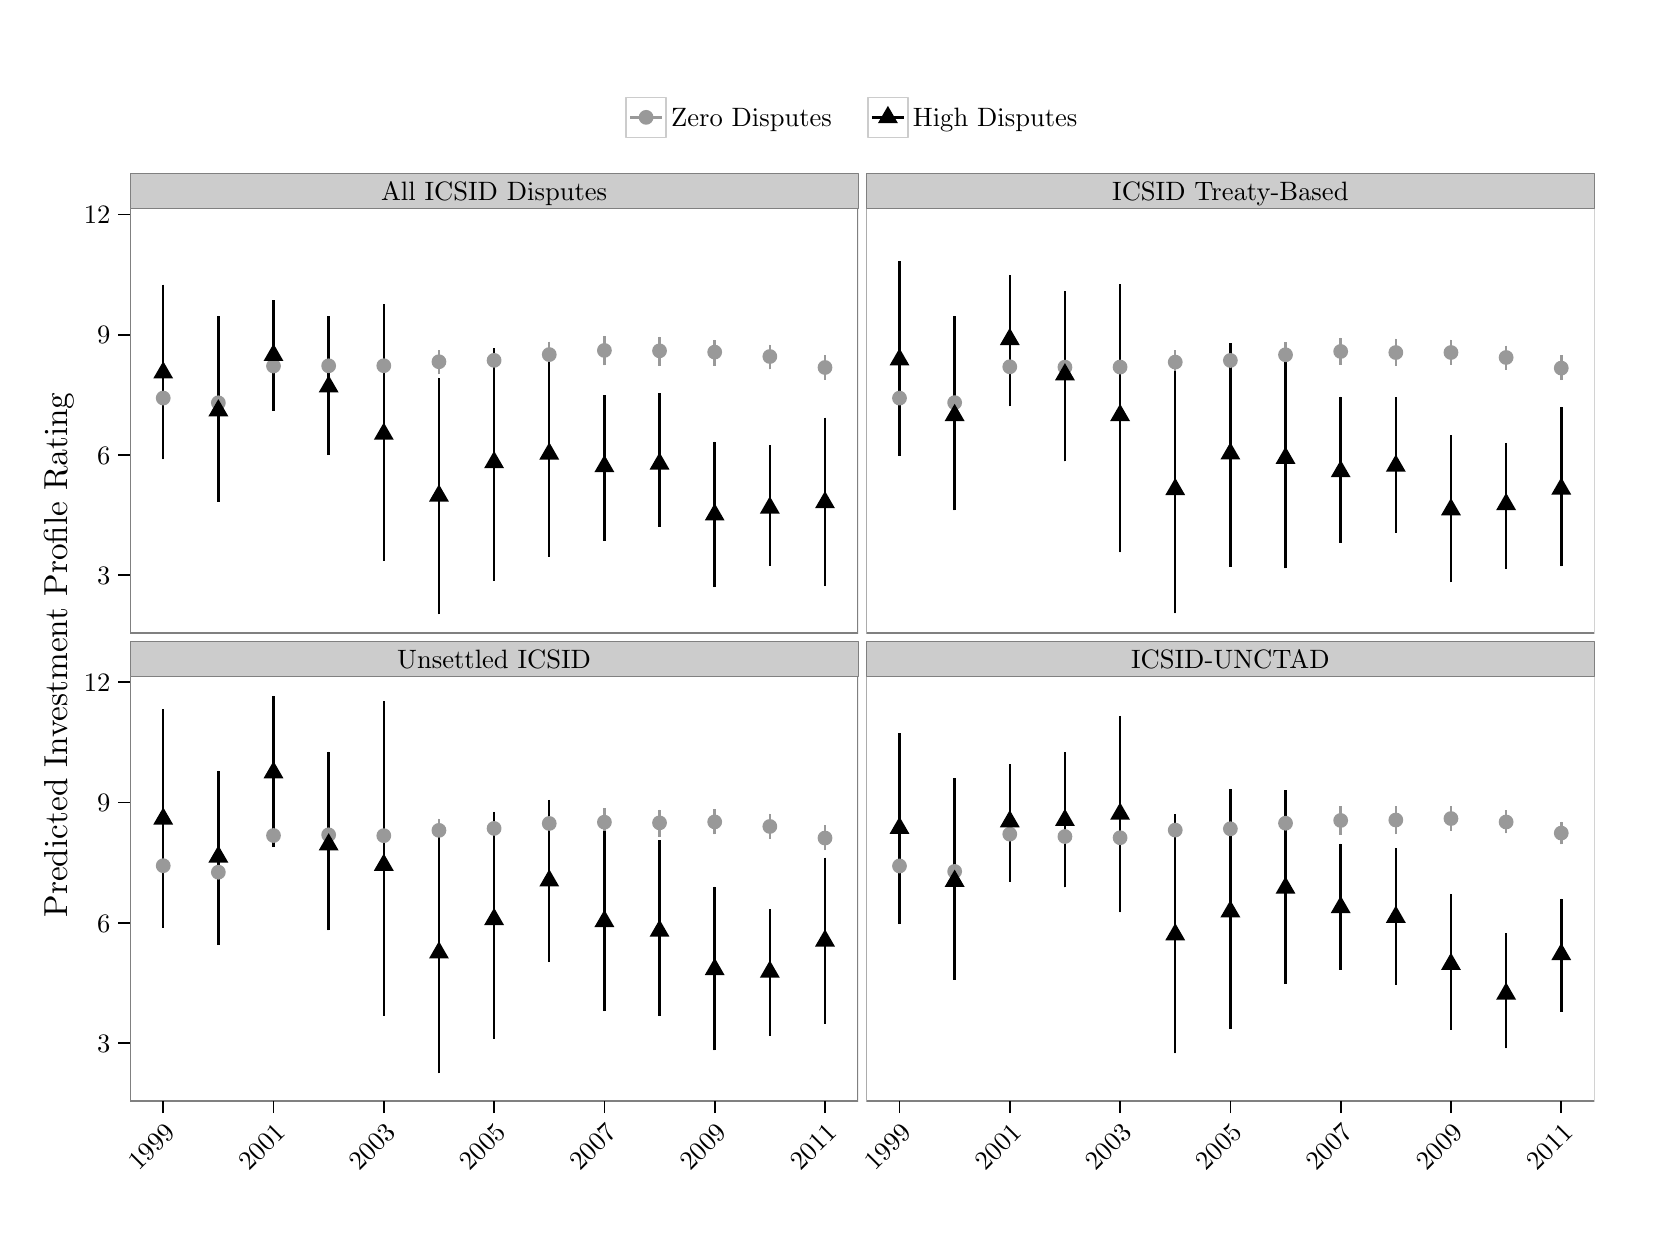
\begin{tikzpicture}[x=1pt,y=1pt]
\definecolor[named]{fillColor}{rgb}{1.00,1.00,1.00}
\path[use as bounding box,fill=fillColor,fill opacity=0.00] (0,0) rectangle (578.16,433.62);
\begin{scope}
\path[clip] (  0.00,  0.00) rectangle (578.16,433.62);
\definecolor[named]{drawColor}{rgb}{1.00,1.00,1.00}
\definecolor[named]{fillColor}{rgb}{1.00,1.00,1.00}

\path[draw=drawColor,line width= 0.6pt,line join=round,line cap=round,fill=fillColor] (  0.00,  0.00) rectangle (578.16,433.62);
\end{scope}
\begin{scope}
\path[clip] ( 37.02,214.77) rectangle (300.06,368.22);
\definecolor[named]{fillColor}{rgb}{1.00,1.00,1.00}

\path[fill=fillColor] ( 37.02,214.77) rectangle (300.06,368.22);
\definecolor[named]{drawColor}{rgb}{0.60,0.60,0.60}
\definecolor[named]{fillColor}{rgb}{0.60,0.60,0.60}

\path[draw=drawColor,line width= 0.9pt,line join=round,fill=fillColor] ( 48.98,293.67) -- ( 48.98,305.59);

\path[draw=drawColor,line width= 0.9pt,line join=round,fill=fillColor] ( 68.90,291.93) -- ( 68.90,304.29);

\path[draw=drawColor,line width= 0.9pt,line join=round,fill=fillColor] ( 88.83,307.70) -- ( 88.83,315.07);

\path[draw=drawColor,line width= 0.9pt,line join=round,fill=fillColor] (108.76,305.93) -- (108.76,317.28);

\path[draw=drawColor,line width= 0.9pt,line join=round,fill=fillColor] (128.69,306.46) -- (128.69,316.72);

\path[draw=drawColor,line width= 0.9pt,line join=round,fill=fillColor] (148.61,308.45) -- (148.61,317.07);

\path[draw=drawColor,line width= 0.9pt,line join=round,fill=fillColor] (168.54,309.24) -- (168.54,317.81);

\path[draw=drawColor,line width= 0.9pt,line join=round,fill=fillColor] (188.47,310.64) -- (188.47,320.16);

\path[draw=drawColor,line width= 0.9pt,line join=round,fill=fillColor] (208.40,311.61) -- (208.40,322.25);

\path[draw=drawColor,line width= 0.9pt,line join=round,fill=fillColor] (228.32,311.45) -- (228.32,321.98);

\path[draw=drawColor,line width= 0.9pt,line join=round,fill=fillColor] (248.25,311.52) -- (248.25,320.82);

\path[draw=drawColor,line width= 0.9pt,line join=round,fill=fillColor] (268.18,310.10) -- (268.18,319.07);

\path[draw=drawColor,line width= 0.9pt,line join=round,fill=fillColor] (288.11,306.38) -- (288.11,315.18);
\definecolor[named]{drawColor}{rgb}{0.00,0.00,0.00}
\definecolor[named]{fillColor}{rgb}{0.00,0.00,0.00}

\path[draw=drawColor,line width= 0.9pt,line join=round,fill=fillColor] ( 48.98,277.65) -- ( 48.98,340.81);

\path[draw=drawColor,line width= 0.9pt,line join=round,fill=fillColor] ( 68.90,262.34) -- ( 68.90,329.49);

\path[draw=drawColor,line width= 0.9pt,line join=round,fill=fillColor] ( 88.83,295.23) -- ( 88.83,335.12);

\path[draw=drawColor,line width= 0.9pt,line join=round,fill=fillColor] (108.76,279.19) -- (108.76,329.36);

\path[draw=drawColor,line width= 0.9pt,line join=round,fill=fillColor] (128.69,240.98) -- (128.69,333.61);

\path[draw=drawColor,line width= 0.9pt,line join=round,fill=fillColor] (148.61,221.74) -- (148.61,307.17);

\path[draw=drawColor,line width= 0.9pt,line join=round,fill=fillColor] (168.54,233.78) -- (168.54,317.86);

\path[draw=drawColor,line width= 0.9pt,line join=round,fill=fillColor] (188.47,242.46) -- (188.47,316.24);

\path[draw=drawColor,line width= 0.9pt,line join=round,fill=fillColor] (208.40,248.30) -- (208.40,300.81);

\path[draw=drawColor,line width= 0.9pt,line join=round,fill=fillColor] (228.32,253.28) -- (228.32,301.49);

\path[draw=drawColor,line width= 0.9pt,line join=round,fill=fillColor] (248.25,231.43) -- (248.25,284.04);

\path[draw=drawColor,line width= 0.9pt,line join=round,fill=fillColor] (268.18,239.20) -- (268.18,282.77);

\path[draw=drawColor,line width= 0.9pt,line join=round,fill=fillColor] (288.11,231.84) -- (288.11,292.68);
\definecolor[named]{fillColor}{rgb}{0.60,0.60,0.60}

\path[fill=fillColor] ( 48.98,299.78) circle (  2.67);
\definecolor[named]{fillColor}{rgb}{0.00,0.00,0.00}

\path[fill=fillColor] ( 48.98,313.08) --
	( 52.57,306.86) --
	( 45.38,306.86) --
	cycle;
\definecolor[named]{fillColor}{rgb}{0.60,0.60,0.60}

\path[fill=fillColor] ( 68.90,298.06) circle (  2.67);
\definecolor[named]{fillColor}{rgb}{0.00,0.00,0.00}

\path[fill=fillColor] ( 68.90,299.40) --
	( 72.50,293.18) --
	( 65.31,293.18) --
	cycle;
\definecolor[named]{fillColor}{rgb}{0.60,0.60,0.60}

\path[fill=fillColor] ( 88.83,311.37) circle (  2.67);
\definecolor[named]{fillColor}{rgb}{0.00,0.00,0.00}

\path[fill=fillColor] ( 88.83,319.41) --
	( 92.42,313.18) --
	( 85.24,313.18) --
	cycle;
\definecolor[named]{fillColor}{rgb}{0.60,0.60,0.60}

\path[fill=fillColor] (108.76,311.43) circle (  2.67);
\definecolor[named]{fillColor}{rgb}{0.00,0.00,0.00}

\path[fill=fillColor] (108.76,308.05) --
	(112.35,301.83) --
	(105.17,301.83) --
	cycle;
\definecolor[named]{fillColor}{rgb}{0.60,0.60,0.60}

\path[fill=fillColor] (128.69,311.46) circle (  2.67);
\definecolor[named]{fillColor}{rgb}{0.00,0.00,0.00}

\path[fill=fillColor] (128.69,290.94) --
	(132.28,284.72) --
	(125.09,284.72) --
	cycle;
\definecolor[named]{fillColor}{rgb}{0.60,0.60,0.60}

\path[fill=fillColor] (148.61,312.90) circle (  2.67);
\definecolor[named]{fillColor}{rgb}{0.00,0.00,0.00}

\path[fill=fillColor] (148.61,268.61) --
	(152.21,262.38) --
	(145.02,262.38) --
	cycle;
\definecolor[named]{fillColor}{rgb}{0.60,0.60,0.60}

\path[fill=fillColor] (168.54,313.40) circle (  2.67);
\definecolor[named]{fillColor}{rgb}{0.00,0.00,0.00}

\path[fill=fillColor] (168.54,280.68) --
	(172.13,274.46) --
	(164.95,274.46) --
	cycle;
\definecolor[named]{fillColor}{rgb}{0.60,0.60,0.60}

\path[fill=fillColor] (188.47,315.49) circle (  2.67);
\definecolor[named]{fillColor}{rgb}{0.00,0.00,0.00}

\path[fill=fillColor] (188.47,283.79) --
	(192.06,277.57) --
	(184.88,277.57) --
	cycle;
\definecolor[named]{fillColor}{rgb}{0.60,0.60,0.60}

\path[fill=fillColor] (208.40,316.99) circle (  2.67);
\definecolor[named]{fillColor}{rgb}{0.00,0.00,0.00}

\path[fill=fillColor] (208.40,279.25) --
	(211.99,273.03) --
	(204.80,273.03) --
	cycle;
\definecolor[named]{fillColor}{rgb}{0.60,0.60,0.60}

\path[fill=fillColor] (228.32,316.84) circle (  2.67);
\definecolor[named]{fillColor}{rgb}{0.00,0.00,0.00}

\path[fill=fillColor] (228.32,280.17) --
	(231.92,273.95) --
	(224.73,273.95) --
	cycle;
\definecolor[named]{fillColor}{rgb}{0.60,0.60,0.60}

\path[fill=fillColor] (248.25,316.38) circle (  2.67);
\definecolor[named]{fillColor}{rgb}{0.00,0.00,0.00}

\path[fill=fillColor] (248.25,261.76) --
	(251.84,255.54) --
	(244.66,255.54) --
	cycle;
\definecolor[named]{fillColor}{rgb}{0.60,0.60,0.60}

\path[fill=fillColor] (268.18,314.79) circle (  2.67);
\definecolor[named]{fillColor}{rgb}{0.00,0.00,0.00}

\path[fill=fillColor] (268.18,264.27) --
	(271.77,258.04) --
	(264.59,258.04) --
	cycle;
\definecolor[named]{fillColor}{rgb}{0.60,0.60,0.60}

\path[fill=fillColor] (288.11,310.83) circle (  2.67);
\definecolor[named]{fillColor}{rgb}{0.00,0.00,0.00}

\path[fill=fillColor] (288.11,266.20) --
	(291.70,259.97) --
	(284.51,259.97) --
	cycle;
\definecolor[named]{drawColor}{rgb}{0.50,0.50,0.50}

\path[draw=drawColor,line width= 0.6pt,line join=round,line cap=round] ( 37.02,214.77) rectangle (300.06,368.22);
\end{scope}
\begin{scope}
\path[clip] (303.07,214.77) rectangle (566.12,368.22);
\definecolor[named]{fillColor}{rgb}{1.00,1.00,1.00}

\path[fill=fillColor] (303.07,214.77) rectangle (566.12,368.22);
\definecolor[named]{drawColor}{rgb}{0.60,0.60,0.60}
\definecolor[named]{fillColor}{rgb}{0.60,0.60,0.60}

\path[draw=drawColor,line width= 0.9pt,line join=round,fill=fillColor] (315.03,293.78) -- (315.03,305.84);

\path[draw=drawColor,line width= 0.9pt,line join=round,fill=fillColor] (334.96,291.95) -- (334.96,304.13);

\path[draw=drawColor,line width= 0.9pt,line join=round,fill=fillColor] (354.88,307.16) -- (354.88,314.84);

\path[draw=drawColor,line width= 0.9pt,line join=round,fill=fillColor] (374.81,305.98) -- (374.81,316.10);

\path[draw=drawColor,line width= 0.9pt,line join=round,fill=fillColor] (394.74,305.73) -- (394.74,316.18);

\path[draw=drawColor,line width= 0.9pt,line join=round,fill=fillColor] (414.67,308.47) -- (414.67,316.99);

\path[draw=drawColor,line width= 0.9pt,line join=round,fill=fillColor] (434.59,309.08) -- (434.59,317.58);

\path[draw=drawColor,line width= 0.9pt,line join=round,fill=fillColor] (454.52,310.77) -- (454.52,319.96);

\path[draw=drawColor,line width= 0.9pt,line join=round,fill=fillColor] (474.45,311.76) -- (474.45,321.65);

\path[draw=drawColor,line width= 0.9pt,line join=round,fill=fillColor] (494.38,311.49) -- (494.38,321.25);

\path[draw=drawColor,line width= 0.9pt,line join=round,fill=fillColor] (514.30,311.80) -- (514.30,320.87);

\path[draw=drawColor,line width= 0.9pt,line join=round,fill=fillColor] (534.23,310.00) -- (534.23,318.75);

\path[draw=drawColor,line width= 0.9pt,line join=round,fill=fillColor] (554.16,306.27) -- (554.16,315.18);
\definecolor[named]{drawColor}{rgb}{0.00,0.00,0.00}
\definecolor[named]{fillColor}{rgb}{0.00,0.00,0.00}

\path[draw=drawColor,line width= 0.9pt,line join=round,fill=fillColor] (315.03,278.99) -- (315.03,349.30);

\path[draw=drawColor,line width= 0.9pt,line join=round,fill=fillColor] (334.96,259.18) -- (334.96,329.45);

\path[draw=drawColor,line width= 0.9pt,line join=round,fill=fillColor] (354.88,296.83) -- (354.88,344.32);

\path[draw=drawColor,line width= 0.9pt,line join=round,fill=fillColor] (374.81,276.90) -- (374.81,338.49);

\path[draw=drawColor,line width= 0.9pt,line join=round,fill=fillColor] (394.74,243.99) -- (394.74,340.82);

\path[draw=drawColor,line width= 0.9pt,line join=round,fill=fillColor] (414.67,221.97) -- (414.67,309.69);

\path[draw=drawColor,line width= 0.9pt,line join=round,fill=fillColor] (434.59,238.83) -- (434.59,319.61);

\path[draw=drawColor,line width= 0.9pt,line join=round,fill=fillColor] (454.52,238.22) -- (454.52,316.91);

\path[draw=drawColor,line width= 0.9pt,line join=round,fill=fillColor] (474.45,247.41) -- (474.45,300.28);

\path[draw=drawColor,line width= 0.9pt,line join=round,fill=fillColor] (494.38,251.06) -- (494.38,300.07);

\path[draw=drawColor,line width= 0.9pt,line join=round,fill=fillColor] (514.30,233.31) -- (514.30,286.29);

\path[draw=drawColor,line width= 0.9pt,line join=round,fill=fillColor] (534.23,238.00) -- (534.23,283.55);

\path[draw=drawColor,line width= 0.9pt,line join=round,fill=fillColor] (554.16,238.96) -- (554.16,296.55);
\definecolor[named]{fillColor}{rgb}{0.60,0.60,0.60}

\path[fill=fillColor] (315.03,299.76) circle (  2.67);
\definecolor[named]{fillColor}{rgb}{0.00,0.00,0.00}

\path[fill=fillColor] (315.03,317.80) --
	(318.62,311.58) --
	(311.44,311.58) --
	cycle;
\definecolor[named]{fillColor}{rgb}{0.60,0.60,0.60}

\path[fill=fillColor] (334.96,298.12) circle (  2.67);
\definecolor[named]{fillColor}{rgb}{0.00,0.00,0.00}

\path[fill=fillColor] (334.96,297.70) --
	(338.55,291.48) --
	(331.36,291.48) --
	cycle;
\definecolor[named]{fillColor}{rgb}{0.60,0.60,0.60}

\path[fill=fillColor] (354.88,311.08) circle (  2.67);
\definecolor[named]{fillColor}{rgb}{0.00,0.00,0.00}

\path[fill=fillColor] (354.88,325.15) --
	(358.48,318.92) --
	(351.29,318.92) --
	cycle;
\definecolor[named]{fillColor}{rgb}{0.60,0.60,0.60}

\path[fill=fillColor] (374.81,310.94) circle (  2.67);
\definecolor[named]{fillColor}{rgb}{0.00,0.00,0.00}

\path[fill=fillColor] (374.81,312.41) --
	(378.40,306.19) --
	(371.22,306.19) --
	cycle;
\definecolor[named]{fillColor}{rgb}{0.60,0.60,0.60}

\path[fill=fillColor] (394.74,310.98) circle (  2.67);
\definecolor[named]{fillColor}{rgb}{0.00,0.00,0.00}

\path[fill=fillColor] (394.74,297.69) --
	(398.33,291.47) --
	(391.15,291.47) --
	cycle;
\definecolor[named]{fillColor}{rgb}{0.60,0.60,0.60}

\path[fill=fillColor] (414.67,312.77) circle (  2.67);
\definecolor[named]{fillColor}{rgb}{0.00,0.00,0.00}

\path[fill=fillColor] (414.67,270.93) --
	(418.26,264.71) --
	(411.07,264.71) --
	cycle;
\definecolor[named]{fillColor}{rgb}{0.60,0.60,0.60}

\path[fill=fillColor] (434.59,313.37) circle (  2.67);
\definecolor[named]{fillColor}{rgb}{0.00,0.00,0.00}

\path[fill=fillColor] (434.59,283.82) --
	(438.19,277.59) --
	(431.00,277.59) --
	cycle;
\definecolor[named]{fillColor}{rgb}{0.60,0.60,0.60}

\path[fill=fillColor] (454.52,315.42) circle (  2.67);
\definecolor[named]{fillColor}{rgb}{0.00,0.00,0.00}

\path[fill=fillColor] (454.52,282.24) --
	(458.11,276.02) --
	(450.93,276.02) --
	cycle;
\definecolor[named]{fillColor}{rgb}{0.60,0.60,0.60}

\path[fill=fillColor] (474.45,316.62) circle (  2.67);
\definecolor[named]{fillColor}{rgb}{0.00,0.00,0.00}

\path[fill=fillColor] (474.45,277.40) --
	(478.04,271.18) --
	(470.86,271.18) --
	cycle;
\definecolor[named]{fillColor}{rgb}{0.60,0.60,0.60}

\path[fill=fillColor] (494.38,316.22) circle (  2.67);
\definecolor[named]{fillColor}{rgb}{0.00,0.00,0.00}

\path[fill=fillColor] (494.38,279.40) --
	(497.97,273.18) --
	(490.78,273.18) --
	cycle;
\definecolor[named]{fillColor}{rgb}{0.60,0.60,0.60}

\path[fill=fillColor] (514.30,316.24) circle (  2.67);
\definecolor[named]{fillColor}{rgb}{0.00,0.00,0.00}

\path[fill=fillColor] (514.30,263.64) --
	(517.90,257.42) --
	(510.71,257.42) --
	cycle;
\definecolor[named]{fillColor}{rgb}{0.60,0.60,0.60}

\path[fill=fillColor] (534.23,314.44) circle (  2.67);
\definecolor[named]{fillColor}{rgb}{0.00,0.00,0.00}

\path[fill=fillColor] (534.23,265.53) --
	(537.82,259.31) --
	(530.64,259.31) --
	cycle;
\definecolor[named]{fillColor}{rgb}{0.60,0.60,0.60}

\path[fill=fillColor] (554.16,310.60) circle (  2.67);
\definecolor[named]{fillColor}{rgb}{0.00,0.00,0.00}

\path[fill=fillColor] (554.16,271.14) --
	(557.75,264.92) --
	(550.57,264.92) --
	cycle;
\definecolor[named]{drawColor}{rgb}{0.50,0.50,0.50}

\path[draw=drawColor,line width= 0.6pt,line join=round,line cap=round] (303.07,214.77) rectangle (566.12,368.22);
\end{scope}
\begin{scope}
\path[clip] ( 37.02, 45.67) rectangle (300.06,199.12);
\definecolor[named]{fillColor}{rgb}{1.00,1.00,1.00}

\path[fill=fillColor] ( 37.02, 45.67) rectangle (300.06,199.12);
\definecolor[named]{drawColor}{rgb}{0.60,0.60,0.60}
\definecolor[named]{fillColor}{rgb}{0.60,0.60,0.60}

\path[draw=drawColor,line width= 0.9pt,line join=round,fill=fillColor] ( 48.98,125.38) -- ( 48.98,136.64);

\path[draw=drawColor,line width= 0.9pt,line join=round,fill=fillColor] ( 68.90,122.62) -- ( 68.90,134.68);

\path[draw=drawColor,line width= 0.9pt,line join=round,fill=fillColor] ( 88.83,137.99) -- ( 88.83,145.38);

\path[draw=drawColor,line width= 0.9pt,line join=round,fill=fillColor] (108.76,136.92) -- (108.76,146.80);

\path[draw=drawColor,line width= 0.9pt,line join=round,fill=fillColor] (128.69,136.43) -- (128.69,146.97);

\path[draw=drawColor,line width= 0.9pt,line join=round,fill=fillColor] (148.61,139.21) -- (148.61,147.84);

\path[draw=drawColor,line width= 0.9pt,line join=round,fill=fillColor] (168.54,139.98) -- (168.54,148.92);

\path[draw=drawColor,line width= 0.9pt,line join=round,fill=fillColor] (188.47,141.35) -- (188.47,150.56);

\path[draw=drawColor,line width= 0.9pt,line join=round,fill=fillColor] (208.40,141.52) -- (208.40,151.53);

\path[draw=drawColor,line width= 0.9pt,line join=round,fill=fillColor] (228.32,141.08) -- (228.32,151.10);

\path[draw=drawColor,line width= 0.9pt,line join=round,fill=fillColor] (248.25,142.10) -- (248.25,151.31);

\path[draw=drawColor,line width= 0.9pt,line join=round,fill=fillColor] (268.18,140.56) -- (268.18,149.61);

\path[draw=drawColor,line width= 0.9pt,line join=round,fill=fillColor] (288.11,136.44) -- (288.11,145.36);
\definecolor[named]{drawColor}{rgb}{0.00,0.00,0.00}
\definecolor[named]{fillColor}{rgb}{0.00,0.00,0.00}

\path[draw=drawColor,line width= 0.9pt,line join=round,fill=fillColor] ( 48.98,108.37) -- ( 48.98,187.25);

\path[draw=drawColor,line width= 0.9pt,line join=round,fill=fillColor] ( 68.90,102.13) -- ( 68.90,165.18);

\path[draw=drawColor,line width= 0.9pt,line join=round,fill=fillColor] ( 88.83,137.47) -- ( 88.83,192.15);

\path[draw=drawColor,line width= 0.9pt,line join=round,fill=fillColor] (108.76,107.39) -- (108.76,171.99);

\path[draw=drawColor,line width= 0.9pt,line join=round,fill=fillColor] (128.69, 76.50) -- (128.69,190.14);

\path[draw=drawColor,line width= 0.9pt,line join=round,fill=fillColor] (148.61, 55.81) -- (148.61,142.68);

\path[draw=drawColor,line width= 0.9pt,line join=round,fill=fillColor] (168.54, 68.20) -- (168.54,150.27);

\path[draw=drawColor,line width= 0.9pt,line join=round,fill=fillColor] (188.47, 95.95) -- (188.47,154.62);

\path[draw=drawColor,line width= 0.9pt,line join=round,fill=fillColor] (208.40, 78.21) -- (208.40,143.42);

\path[draw=drawColor,line width= 0.9pt,line join=round,fill=fillColor] (228.32, 76.53) -- (228.32,140.01);

\path[draw=drawColor,line width= 0.9pt,line join=round,fill=fillColor] (248.25, 64.08) -- (248.25,123.27);

\path[draw=drawColor,line width= 0.9pt,line join=round,fill=fillColor] (268.18, 69.38) -- (268.18,115.03);

\path[draw=drawColor,line width= 0.9pt,line join=round,fill=fillColor] (288.11, 73.63) -- (288.11,133.71);
\definecolor[named]{fillColor}{rgb}{0.60,0.60,0.60}

\path[fill=fillColor] ( 48.98,130.79) circle (  2.67);
\definecolor[named]{fillColor}{rgb}{0.00,0.00,0.00}

\path[fill=fillColor] ( 48.98,151.88) --
	( 52.57,145.66) --
	( 45.38,145.66) --
	cycle;
\definecolor[named]{fillColor}{rgb}{0.60,0.60,0.60}

\path[fill=fillColor] ( 68.90,128.45) circle (  2.67);
\definecolor[named]{fillColor}{rgb}{0.00,0.00,0.00}

\path[fill=fillColor] ( 68.90,138.16) --
	( 72.50,131.93) --
	( 65.31,131.93) --
	cycle;
\definecolor[named]{fillColor}{rgb}{0.60,0.60,0.60}

\path[fill=fillColor] ( 88.83,141.70) circle (  2.67);
\definecolor[named]{fillColor}{rgb}{0.00,0.00,0.00}

\path[fill=fillColor] ( 88.83,168.61) --
	( 92.42,162.39) --
	( 85.24,162.39) --
	cycle;
\definecolor[named]{fillColor}{rgb}{0.60,0.60,0.60}

\path[fill=fillColor] (108.76,141.95) circle (  2.67);
\definecolor[named]{fillColor}{rgb}{0.00,0.00,0.00}

\path[fill=fillColor] (108.76,142.56) --
	(112.35,136.34) --
	(105.17,136.34) --
	cycle;
\definecolor[named]{fillColor}{rgb}{0.60,0.60,0.60}

\path[fill=fillColor] (128.69,141.65) circle (  2.67);
\definecolor[named]{fillColor}{rgb}{0.00,0.00,0.00}

\path[fill=fillColor] (128.69,135.19) --
	(132.28,128.97) --
	(125.09,128.97) --
	cycle;
\definecolor[named]{fillColor}{rgb}{0.60,0.60,0.60}

\path[fill=fillColor] (148.61,143.57) circle (  2.67);
\definecolor[named]{fillColor}{rgb}{0.00,0.00,0.00}

\path[fill=fillColor] (148.61,103.50) --
	(152.21, 97.28) --
	(145.02, 97.28) --
	cycle;
\definecolor[named]{fillColor}{rgb}{0.60,0.60,0.60}

\path[fill=fillColor] (168.54,144.27) circle (  2.67);
\definecolor[named]{fillColor}{rgb}{0.00,0.00,0.00}

\path[fill=fillColor] (168.54,115.58) --
	(172.13,109.36) --
	(164.95,109.36) --
	cycle;
\definecolor[named]{fillColor}{rgb}{0.60,0.60,0.60}

\path[fill=fillColor] (188.47,146.06) circle (  2.67);
\definecolor[named]{fillColor}{rgb}{0.00,0.00,0.00}

\path[fill=fillColor] (188.47,129.51) --
	(192.06,123.29) --
	(184.88,123.29) --
	cycle;
\definecolor[named]{fillColor}{rgb}{0.60,0.60,0.60}

\path[fill=fillColor] (208.40,146.52) circle (  2.67);
\definecolor[named]{fillColor}{rgb}{0.00,0.00,0.00}

\path[fill=fillColor] (208.40,114.87) --
	(211.99,108.64) --
	(204.80,108.64) --
	cycle;
\definecolor[named]{fillColor}{rgb}{0.60,0.60,0.60}

\path[fill=fillColor] (228.32,146.28) circle (  2.67);
\definecolor[named]{fillColor}{rgb}{0.00,0.00,0.00}

\path[fill=fillColor] (228.32,111.36) --
	(231.92,105.14) --
	(224.73,105.14) --
	cycle;
\definecolor[named]{fillColor}{rgb}{0.60,0.60,0.60}

\path[fill=fillColor] (248.25,146.63) circle (  2.67);
\definecolor[named]{fillColor}{rgb}{0.00,0.00,0.00}

\path[fill=fillColor] (248.25, 97.50) --
	(251.84, 91.27) --
	(244.66, 91.27) --
	cycle;
\definecolor[named]{fillColor}{rgb}{0.60,0.60,0.60}

\path[fill=fillColor] (268.18,144.98) circle (  2.67);
\definecolor[named]{fillColor}{rgb}{0.00,0.00,0.00}

\path[fill=fillColor] (268.18, 96.58) --
	(271.77, 90.36) --
	(264.59, 90.36) --
	cycle;
\definecolor[named]{fillColor}{rgb}{0.60,0.60,0.60}

\path[fill=fillColor] (288.11,140.79) circle (  2.67);
\definecolor[named]{fillColor}{rgb}{0.00,0.00,0.00}

\path[fill=fillColor] (288.11,107.82) --
	(291.70,101.60) --
	(284.51,101.60) --
	cycle;
\definecolor[named]{drawColor}{rgb}{0.50,0.50,0.50}

\path[draw=drawColor,line width= 0.6pt,line join=round,line cap=round] ( 37.02, 45.67) rectangle (300.06,199.12);
\end{scope}
\begin{scope}
\path[clip] (303.07, 45.67) rectangle (566.12,199.12);
\definecolor[named]{fillColor}{rgb}{1.00,1.00,1.00}

\path[fill=fillColor] (303.07, 45.67) rectangle (566.12,199.12);
\definecolor[named]{drawColor}{rgb}{0.60,0.60,0.60}
\definecolor[named]{fillColor}{rgb}{0.60,0.60,0.60}

\path[draw=drawColor,line width= 0.9pt,line join=round,fill=fillColor] (315.03,124.77) -- (315.03,136.40);

\path[draw=drawColor,line width= 0.9pt,line join=round,fill=fillColor] (334.96,122.55) -- (334.96,134.49);

\path[draw=drawColor,line width= 0.9pt,line join=round,fill=fillColor] (354.88,138.58) -- (354.88,146.09);

\path[draw=drawColor,line width= 0.9pt,line join=round,fill=fillColor] (374.81,135.46) -- (374.81,146.59);

\path[draw=drawColor,line width= 0.9pt,line join=round,fill=fillColor] (394.74,135.88) -- (394.74,145.95);

\path[draw=drawColor,line width= 0.9pt,line join=round,fill=fillColor] (414.67,139.39) -- (414.67,147.97);

\path[draw=drawColor,line width= 0.9pt,line join=round,fill=fillColor] (434.59,139.78) -- (434.59,148.45);

\path[draw=drawColor,line width= 0.9pt,line join=round,fill=fillColor] (454.52,141.53) -- (454.52,150.88);

\path[draw=drawColor,line width= 0.9pt,line join=round,fill=fillColor] (474.45,141.91) -- (474.45,152.29);

\path[draw=drawColor,line width= 0.9pt,line join=round,fill=fillColor] (494.38,142.20) -- (494.38,152.36);

\path[draw=drawColor,line width= 0.9pt,line join=round,fill=fillColor] (514.30,143.35) -- (514.30,152.28);

\path[draw=drawColor,line width= 0.9pt,line join=round,fill=fillColor] (534.23,142.45) -- (534.23,150.85);

\path[draw=drawColor,line width= 0.9pt,line join=round,fill=fillColor] (554.16,138.48) -- (554.16,146.68);
\definecolor[named]{drawColor}{rgb}{0.00,0.00,0.00}
\definecolor[named]{fillColor}{rgb}{0.00,0.00,0.00}

\path[draw=drawColor,line width= 0.9pt,line join=round,fill=fillColor] (315.03,109.70) -- (315.03,178.73);

\path[draw=drawColor,line width= 0.9pt,line join=round,fill=fillColor] (334.96, 89.60) -- (334.96,162.56);

\path[draw=drawColor,line width= 0.9pt,line join=round,fill=fillColor] (354.88,124.91) -- (354.88,167.47);

\path[draw=drawColor,line width= 0.9pt,line join=round,fill=fillColor] (374.81,122.92) -- (374.81,171.79);

\path[draw=drawColor,line width= 0.9pt,line join=round,fill=fillColor] (394.74,113.96) -- (394.74,184.97);

\path[draw=drawColor,line width= 0.9pt,line join=round,fill=fillColor] (414.67, 62.98) -- (414.67,149.42);

\path[draw=drawColor,line width= 0.9pt,line join=round,fill=fillColor] (434.59, 71.72) -- (434.59,158.52);

\path[draw=drawColor,line width= 0.9pt,line join=round,fill=fillColor] (454.52, 88.23) -- (454.52,158.15);

\path[draw=drawColor,line width= 0.9pt,line join=round,fill=fillColor] (474.45, 93.25) -- (474.45,138.81);

\path[draw=drawColor,line width= 0.9pt,line join=round,fill=fillColor] (494.38, 87.78) -- (494.38,137.21);

\path[draw=drawColor,line width= 0.9pt,line join=round,fill=fillColor] (514.30, 71.48) -- (514.30,120.63);

\path[draw=drawColor,line width= 0.9pt,line join=round,fill=fillColor] (534.23, 64.78) -- (534.23,106.32);

\path[draw=drawColor,line width= 0.9pt,line join=round,fill=fillColor] (554.16, 77.99) -- (554.16,118.94);
\definecolor[named]{fillColor}{rgb}{0.60,0.60,0.60}

\path[fill=fillColor] (315.03,130.70) circle (  2.67);
\definecolor[named]{fillColor}{rgb}{0.00,0.00,0.00}

\path[fill=fillColor] (315.03,148.52) --
	(318.62,142.30) --
	(311.44,142.30) --
	cycle;
\definecolor[named]{fillColor}{rgb}{0.60,0.60,0.60}

\path[fill=fillColor] (334.96,128.73) circle (  2.67);
\definecolor[named]{fillColor}{rgb}{0.00,0.00,0.00}

\path[fill=fillColor] (334.96,129.39) --
	(338.55,123.16) --
	(331.36,123.16) --
	cycle;
\definecolor[named]{fillColor}{rgb}{0.60,0.60,0.60}

\path[fill=fillColor] (354.88,142.20) circle (  2.67);
\definecolor[named]{fillColor}{rgb}{0.00,0.00,0.00}

\path[fill=fillColor] (354.88,150.89) --
	(358.48,144.67) --
	(351.29,144.67) --
	cycle;
\definecolor[named]{fillColor}{rgb}{0.60,0.60,0.60}

\path[fill=fillColor] (374.81,141.34) circle (  2.67);
\definecolor[named]{fillColor}{rgb}{0.00,0.00,0.00}

\path[fill=fillColor] (374.81,151.38) --
	(378.40,145.16) --
	(371.22,145.16) --
	cycle;
\definecolor[named]{fillColor}{rgb}{0.60,0.60,0.60}

\path[fill=fillColor] (394.74,140.90) circle (  2.67);
\definecolor[named]{fillColor}{rgb}{0.00,0.00,0.00}

\path[fill=fillColor] (394.74,153.66) --
	(398.33,147.43) --
	(391.15,147.43) --
	cycle;
\definecolor[named]{fillColor}{rgb}{0.60,0.60,0.60}

\path[fill=fillColor] (414.67,143.66) circle (  2.67);
\definecolor[named]{fillColor}{rgb}{0.00,0.00,0.00}

\path[fill=fillColor] (414.67,110.05) --
	(418.26,103.83) --
	(411.07,103.83) --
	cycle;
\definecolor[named]{fillColor}{rgb}{0.60,0.60,0.60}

\path[fill=fillColor] (434.59,144.13) circle (  2.67);
\definecolor[named]{fillColor}{rgb}{0.00,0.00,0.00}

\path[fill=fillColor] (434.59,118.36) --
	(438.19,112.14) --
	(431.00,112.14) --
	cycle;
\definecolor[named]{fillColor}{rgb}{0.60,0.60,0.60}

\path[fill=fillColor] (454.52,146.15) circle (  2.67);
\definecolor[named]{fillColor}{rgb}{0.00,0.00,0.00}

\path[fill=fillColor] (454.52,126.92) --
	(458.11,120.70) --
	(450.93,120.70) --
	cycle;
\definecolor[named]{fillColor}{rgb}{0.60,0.60,0.60}

\path[fill=fillColor] (474.45,147.15) circle (  2.67);
\definecolor[named]{fillColor}{rgb}{0.00,0.00,0.00}

\path[fill=fillColor] (474.45,119.91) --
	(478.04,113.69) --
	(470.86,113.69) --
	cycle;
\definecolor[named]{fillColor}{rgb}{0.60,0.60,0.60}

\path[fill=fillColor] (494.38,147.30) circle (  2.67);
\definecolor[named]{fillColor}{rgb}{0.00,0.00,0.00}

\path[fill=fillColor] (494.38,116.40) --
	(497.97,110.17) --
	(490.78,110.17) --
	cycle;
\definecolor[named]{fillColor}{rgb}{0.60,0.60,0.60}

\path[fill=fillColor] (514.30,147.83) circle (  2.67);
\definecolor[named]{fillColor}{rgb}{0.00,0.00,0.00}

\path[fill=fillColor] (514.30, 99.36) --
	(517.90, 93.13) --
	(510.71, 93.13) --
	cycle;
\definecolor[named]{fillColor}{rgb}{0.60,0.60,0.60}

\path[fill=fillColor] (534.23,146.59) circle (  2.67);
\definecolor[named]{fillColor}{rgb}{0.00,0.00,0.00}

\path[fill=fillColor] (534.23, 88.64) --
	(537.82, 82.42) --
	(530.64, 82.42) --
	cycle;
\definecolor[named]{fillColor}{rgb}{0.60,0.60,0.60}

\path[fill=fillColor] (554.16,142.58) circle (  2.67);
\definecolor[named]{fillColor}{rgb}{0.00,0.00,0.00}

\path[fill=fillColor] (554.16,102.90) --
	(557.75, 96.68) --
	(550.57, 96.68) --
	cycle;
\definecolor[named]{drawColor}{rgb}{0.50,0.50,0.50}

\path[draw=drawColor,line width= 0.6pt,line join=round,line cap=round] (303.07, 45.67) rectangle (566.12,199.12);
\end{scope}
\begin{scope}
\path[clip] (  0.00,  0.00) rectangle (578.16,433.62);
\definecolor[named]{drawColor}{rgb}{0.50,0.50,0.50}
\definecolor[named]{fillColor}{rgb}{0.80,0.80,0.80}

\path[draw=drawColor,line width= 0.2pt,line join=round,line cap=round,fill=fillColor] ( 37.02,368.22) rectangle (300.06,380.85);
\definecolor[named]{drawColor}{rgb}{0.00,0.00,0.00}

\node[text=drawColor,anchor=base,inner sep=0pt, outer sep=0pt, scale=  0.96] at (168.54,371.23) {All ICSID Disputes};
\end{scope}
\begin{scope}
\path[clip] (  0.00,  0.00) rectangle (578.16,433.62);
\definecolor[named]{drawColor}{rgb}{0.50,0.50,0.50}
\definecolor[named]{fillColor}{rgb}{0.80,0.80,0.80}

\path[draw=drawColor,line width= 0.2pt,line join=round,line cap=round,fill=fillColor] (303.07,368.22) rectangle (566.12,380.85);
\definecolor[named]{drawColor}{rgb}{0.00,0.00,0.00}

\node[text=drawColor,anchor=base,inner sep=0pt, outer sep=0pt, scale=  0.96] at (434.59,371.23) {ICSID Treaty-Based};
\end{scope}
\begin{scope}
\path[clip] (  0.00,  0.00) rectangle (578.16,433.62);
\definecolor[named]{drawColor}{rgb}{0.50,0.50,0.50}
\definecolor[named]{fillColor}{rgb}{0.80,0.80,0.80}

\path[draw=drawColor,line width= 0.2pt,line join=round,line cap=round,fill=fillColor] ( 37.02,199.12) rectangle (300.06,211.75);
\definecolor[named]{drawColor}{rgb}{0.00,0.00,0.00}

\node[text=drawColor,anchor=base,inner sep=0pt, outer sep=0pt, scale=  0.96] at (168.54,202.13) {Unsettled ICSID};
\end{scope}
\begin{scope}
\path[clip] (  0.00,  0.00) rectangle (578.16,433.62);
\definecolor[named]{drawColor}{rgb}{0.50,0.50,0.50}
\definecolor[named]{fillColor}{rgb}{0.80,0.80,0.80}

\path[draw=drawColor,line width= 0.2pt,line join=round,line cap=round,fill=fillColor] (303.07,199.12) rectangle (566.12,211.75);
\definecolor[named]{drawColor}{rgb}{0.00,0.00,0.00}

\node[text=drawColor,anchor=base,inner sep=0pt, outer sep=0pt, scale=  0.96] at (434.59,202.13) {ICSID-UNCTAD};
\end{scope}
\begin{scope}
\path[clip] (  0.00,  0.00) rectangle (578.16,433.62);
\definecolor[named]{drawColor}{rgb}{0.00,0.00,0.00}

\node[text=drawColor,anchor=base east,inner sep=0pt, outer sep=0pt, scale=  0.96] at ( 29.91,232.42) {3};

\node[text=drawColor,anchor=base east,inner sep=0pt, outer sep=0pt, scale=  0.96] at ( 29.91,275.90) {6};

\node[text=drawColor,anchor=base east,inner sep=0pt, outer sep=0pt, scale=  0.96] at ( 29.91,319.38) {9};

\node[text=drawColor,anchor=base east,inner sep=0pt, outer sep=0pt, scale=  0.96] at ( 29.91,362.86) {12};
\end{scope}
\begin{scope}
\path[clip] (  0.00,  0.00) rectangle (578.16,433.62);
\definecolor[named]{drawColor}{rgb}{0.00,0.00,0.00}

\path[draw=drawColor,line width= 0.6pt,line join=round] ( 32.75,235.73) --
	( 37.02,235.73);

\path[draw=drawColor,line width= 0.6pt,line join=round] ( 32.75,279.21) --
	( 37.02,279.21);

\path[draw=drawColor,line width= 0.6pt,line join=round] ( 32.75,322.68) --
	( 37.02,322.68);

\path[draw=drawColor,line width= 0.6pt,line join=round] ( 32.75,366.16) --
	( 37.02,366.16);
\end{scope}
\begin{scope}
\path[clip] (  0.00,  0.00) rectangle (578.16,433.62);
\definecolor[named]{drawColor}{rgb}{0.00,0.00,0.00}

\node[text=drawColor,anchor=base east,inner sep=0pt, outer sep=0pt, scale=  0.96] at ( 29.91, 63.33) {3};

\node[text=drawColor,anchor=base east,inner sep=0pt, outer sep=0pt, scale=  0.96] at ( 29.91,106.81) {6};

\node[text=drawColor,anchor=base east,inner sep=0pt, outer sep=0pt, scale=  0.96] at ( 29.91,150.28) {9};

\node[text=drawColor,anchor=base east,inner sep=0pt, outer sep=0pt, scale=  0.96] at ( 29.91,193.76) {12};
\end{scope}
\begin{scope}
\path[clip] (  0.00,  0.00) rectangle (578.16,433.62);
\definecolor[named]{drawColor}{rgb}{0.00,0.00,0.00}

\path[draw=drawColor,line width= 0.6pt,line join=round] ( 32.75, 66.63) --
	( 37.02, 66.63);

\path[draw=drawColor,line width= 0.6pt,line join=round] ( 32.75,110.11) --
	( 37.02,110.11);

\path[draw=drawColor,line width= 0.6pt,line join=round] ( 32.75,153.59) --
	( 37.02,153.59);

\path[draw=drawColor,line width= 0.6pt,line join=round] ( 32.75,197.07) --
	( 37.02,197.07);
\end{scope}
\begin{scope}
\path[clip] (  0.00,  0.00) rectangle (578.16,433.62);
\definecolor[named]{drawColor}{rgb}{0.00,0.00,0.00}

\path[draw=drawColor,line width= 0.6pt,line join=round] ( 48.98, 41.40) --
	( 48.98, 45.67);

\path[draw=drawColor,line width= 0.6pt,line join=round] ( 88.83, 41.40) --
	( 88.83, 45.67);

\path[draw=drawColor,line width= 0.6pt,line join=round] (128.69, 41.40) --
	(128.69, 45.67);

\path[draw=drawColor,line width= 0.6pt,line join=round] (168.54, 41.40) --
	(168.54, 45.67);

\path[draw=drawColor,line width= 0.6pt,line join=round] (208.40, 41.40) --
	(208.40, 45.67);

\path[draw=drawColor,line width= 0.6pt,line join=round] (248.25, 41.40) --
	(248.25, 45.67);

\path[draw=drawColor,line width= 0.6pt,line join=round] (288.11, 41.40) --
	(288.11, 45.67);
\end{scope}
\begin{scope}
\path[clip] (  0.00,  0.00) rectangle (578.16,433.62);
\definecolor[named]{drawColor}{rgb}{0.00,0.00,0.00}

\node[text=drawColor,rotate= 45.00,anchor=base east,inner sep=0pt, outer sep=0pt, scale=  0.96] at ( 53.65, 33.88) {1999};

\node[text=drawColor,rotate= 45.00,anchor=base east,inner sep=0pt, outer sep=0pt, scale=  0.96] at ( 93.51, 33.88) {2001};

\node[text=drawColor,rotate= 45.00,anchor=base east,inner sep=0pt, outer sep=0pt, scale=  0.96] at (133.36, 33.88) {2003};

\node[text=drawColor,rotate= 45.00,anchor=base east,inner sep=0pt, outer sep=0pt, scale=  0.96] at (173.22, 33.88) {2005};

\node[text=drawColor,rotate= 45.00,anchor=base east,inner sep=0pt, outer sep=0pt, scale=  0.96] at (213.07, 33.88) {2007};

\node[text=drawColor,rotate= 45.00,anchor=base east,inner sep=0pt, outer sep=0pt, scale=  0.96] at (252.93, 33.88) {2009};

\node[text=drawColor,rotate= 45.00,anchor=base east,inner sep=0pt, outer sep=0pt, scale=  0.96] at (292.78, 33.88) {2011};
\end{scope}
\begin{scope}
\path[clip] (  0.00,  0.00) rectangle (578.16,433.62);
\definecolor[named]{drawColor}{rgb}{0.00,0.00,0.00}

\path[draw=drawColor,line width= 0.6pt,line join=round] (315.03, 41.40) --
	(315.03, 45.67);

\path[draw=drawColor,line width= 0.6pt,line join=round] (354.88, 41.40) --
	(354.88, 45.67);

\path[draw=drawColor,line width= 0.6pt,line join=round] (394.74, 41.40) --
	(394.74, 45.67);

\path[draw=drawColor,line width= 0.6pt,line join=round] (434.59, 41.40) --
	(434.59, 45.67);

\path[draw=drawColor,line width= 0.6pt,line join=round] (474.45, 41.40) --
	(474.45, 45.67);

\path[draw=drawColor,line width= 0.6pt,line join=round] (514.30, 41.40) --
	(514.30, 45.67);

\path[draw=drawColor,line width= 0.6pt,line join=round] (554.16, 41.40) --
	(554.16, 45.67);
\end{scope}
\begin{scope}
\path[clip] (  0.00,  0.00) rectangle (578.16,433.62);
\definecolor[named]{drawColor}{rgb}{0.00,0.00,0.00}

\node[text=drawColor,rotate= 45.00,anchor=base east,inner sep=0pt, outer sep=0pt, scale=  0.96] at (319.71, 33.88) {1999};

\node[text=drawColor,rotate= 45.00,anchor=base east,inner sep=0pt, outer sep=0pt, scale=  0.96] at (359.56, 33.88) {2001};

\node[text=drawColor,rotate= 45.00,anchor=base east,inner sep=0pt, outer sep=0pt, scale=  0.96] at (399.41, 33.88) {2003};

\node[text=drawColor,rotate= 45.00,anchor=base east,inner sep=0pt, outer sep=0pt, scale=  0.96] at (439.27, 33.88) {2005};

\node[text=drawColor,rotate= 45.00,anchor=base east,inner sep=0pt, outer sep=0pt, scale=  0.96] at (479.12, 33.88) {2007};

\node[text=drawColor,rotate= 45.00,anchor=base east,inner sep=0pt, outer sep=0pt, scale=  0.96] at (518.98, 33.88) {2009};

\node[text=drawColor,rotate= 45.00,anchor=base east,inner sep=0pt, outer sep=0pt, scale=  0.96] at (558.83, 33.88) {2011};
\end{scope}
\begin{scope}
\path[clip] (  0.00,  0.00) rectangle (578.16,433.62);
\definecolor[named]{drawColor}{rgb}{0.00,0.00,0.00}

\node[text=drawColor,rotate= 90.00,anchor=base,inner sep=0pt, outer sep=0pt, scale=  1.20] at ( 14.29,206.94) {Predicted Investment Profile Rating};
\end{scope}
\begin{scope}
\path[clip] (  0.00,  0.00) rectangle (578.16,433.62);
\definecolor[named]{fillColor}{rgb}{1.00,1.00,1.00}

\path[fill=fillColor] (208.36,389.72) rectangle (394.78,412.71);
\end{scope}
\begin{scope}
\path[clip] (  0.00,  0.00) rectangle (578.16,433.62);
\definecolor[named]{drawColor}{rgb}{0.80,0.80,0.80}
\definecolor[named]{fillColor}{rgb}{1.00,1.00,1.00}

\path[draw=drawColor,line width= 0.6pt,line join=round,line cap=round,fill=fillColor] (216.24,393.99) rectangle (230.69,408.44);
\end{scope}
\begin{scope}
\path[clip] (  0.00,  0.00) rectangle (578.16,433.62);
\definecolor[named]{drawColor}{rgb}{0.60,0.60,0.60}

\path[draw=drawColor,line width= 0.9pt,line join=round] (217.68,401.21) -- (229.25,401.21);
\end{scope}
\begin{scope}
\path[clip] (  0.00,  0.00) rectangle (578.16,433.62);
\definecolor[named]{fillColor}{rgb}{0.60,0.60,0.60}

\path[fill=fillColor] (223.47,401.21) circle (  2.67);
\end{scope}
\begin{scope}
\path[clip] (  0.00,  0.00) rectangle (578.16,433.62);
\definecolor[named]{drawColor}{rgb}{0.80,0.80,0.80}
\definecolor[named]{fillColor}{rgb}{1.00,1.00,1.00}

\path[draw=drawColor,line width= 0.6pt,line join=round,line cap=round,fill=fillColor] (303.62,393.99) rectangle (318.08,408.44);
\end{scope}
\begin{scope}
\path[clip] (  0.00,  0.00) rectangle (578.16,433.62);
\definecolor[named]{drawColor}{rgb}{0.00,0.00,0.00}

\path[draw=drawColor,line width= 0.9pt,line join=round] (305.07,401.21) -- (316.63,401.21);
\end{scope}
\begin{scope}
\path[clip] (  0.00,  0.00) rectangle (578.16,433.62);
\definecolor[named]{fillColor}{rgb}{0.00,0.00,0.00}

\path[fill=fillColor] (310.85,405.36) --
	(314.44,399.14) --
	(307.26,399.14) --
	cycle;
\end{scope}
\begin{scope}
\path[clip] (  0.00,  0.00) rectangle (578.16,433.62);
\definecolor[named]{drawColor}{rgb}{0.00,0.00,0.00}

\node[text=drawColor,anchor=base west,inner sep=0pt, outer sep=0pt, scale=  0.96] at (232.50,397.91) {Zero Disputes $\; \; \;$};
\end{scope}
\begin{scope}
\path[clip] (  0.00,  0.00) rectangle (578.16,433.62);
\definecolor[named]{drawColor}{rgb}{0.00,0.00,0.00}

\node[text=drawColor,anchor=base west,inner sep=0pt, outer sep=0pt, scale=  0.96] at (319.89,397.91) {High Disputes $\; \; \;$};
\end{scope}
\end{tikzpicture}
}
	\caption*{Note: Each line here shows the mean prediction and 95\% interval around a given scenario using the pooled yearly level regression results. The grey line and circle denote the scenario in which all control variables are set to their median and disputes is set to zero. The black line and triangle denote teh scenario in which all control variables are set to their median and the disputes variable is set to its 99th percentile. Results were obtained by using simulations that accounted for inferential uncertainty. }
\end{figure}
\FloatBarrier

Looking across the results shown in this figure, we can see that pre-2007, the predicted investment profile ratings given these two scenarios practically overlap. After 2007, however, we can clearly see a divergence in the reputation of countries that have faced disputes and those have not. Countries that have gone without facing disputes typically receive investment profile ratings of 8, while those that have had a high number of disputes within the past two years have predicted ratings that are almost two points less. 

% \newpage

\section*{Increasing Information and Media Attention}

The preceding empirical results are consistent with the argument that reputational enforcement of treaty commitments is contingent on institutional design and associated information costs. In accordance with theoretical expectation, the impact of investor-state disputes has been relatively marginal over the broader time period of our analysis, and reputational effects only begin to materialize since 2007. The obvious question is what accounts for this trend? Has information about ISDS processes expanded significantly over time, buttressing our theoretical expectations about the importance of information flows? We cite three sources of evidence about a change in information availability in support of such a claim. 

First, there has been a growing amount of publicity in recent years about ICSID cases and the arbitration tribunal as a whole. Figure \ref{fig:icsidMedia} shows the results of a LexisNexis search on mentions of ICSID disputes in international newspaper sources from 1974 to 2011. The lack of media mentions between 1974 and 1990 may simply result from a lack of online media sources; however, that same argument cannot be used to explain the paucity of mentions since the 1990s. Further even after the number of disputes brought before ICSID dramatically increased in the early 2000s, mentions of ICSID in the media did not meaningfully pick up until 2007. Since 2007 though the number of ICSID related articles in newspapers has increased dramatically, with almost 200 stories filed in 2014. This growth in media coverage is consistent with the previous analysis showing a change in the impact of dispute involvement on reputation in recent years.

\begin{figure}[ht]
	\vspace{4cm}
	\centering
	\caption{Newspaper Mentions of ICSID}
	\label{fig:icsidMedia}
	\resizebox{1\textwidth}{!}{\input{graphics/histICSID}}
	\caption*{Note: The height of the grey bars denotes the number of times ICSID was mentioned in a newspaper source in that year from 1974 to 2011, while the dark line represents a count of the number of ICSID disputes brought in that year.}
\end{figure}
\FloatBarrier

Second, since the early 2000s, there has been a dramatic expansion of electronic services monitoring ISDS processes. Table \ref{tab:disputeSites} lists a number of these sources and the date on which they began reporting. 

\begin{table}[ht]
\centering
\caption{Listing of web-based services monitoring ICSID processes}
\label{tab:disputeSites}
\begin{tabular}{lc}
	\hline\hline
	Source & Year Established \\
	\hline
	Investment Treaty News & 2002 \\
	Transnational Dispute Management & 2003 \\
	Investment Treaty Arbitration & 2004 \\
	Global Arbitration Review & 2006 \\
	Investment Arbitration Reporter & 2008 \\
	International Arbitration Database & 2008 \\
	Kluwer Arbitration Blog & 2009 \\
	Investor-State LawGuide & 2011 \\
	International Investment Arbitration & 2011 \\
	\hline\hline
\end{tabular}
\end{table}
\FloatBarrier

Third, since 2006 the ICSID has adopted new rules regarding transparency. Of particular importance are amendments to the ICSID's arbitration rules introduced in 2006, which mandate the Centre to publish excerpts of the legal reasoning applied by arbitration tribunals in reaching their decisions in specific cases.\footnote{\citet{yackee20112006,antonietti:2006}} Prior to this point, information about dispute arbitrations was only available with the consent of both parties. UNCITRAL has also recently adopted new rules on transparency effective April 1, 2014, although they only apply to treaties concluded prior to that date at the agreement of the disputing parties.\footnote{\citet{uncitral:2013}: 33-40 } It seems reasonable to assume that all three sets of changes have led to increased awareness of the cases brought before arbitration tribunals and enhanced the reputational consequences of investment dispute involvement.

\section*{Short and Long Term Effects}

The main limitations of the preceding results are that they do not directly address the question of reputational \textit{change} nor allow us to distinguish between the short and long-term effects of alleged treaty violations. For this reason, we probe the impact of investment disputes further below on the basis of an error correction model (ECM). Contrary, to Allee and Peinhardt, who assert ``once an investment dispute emerges, investors will rethink their assessments of political risk,'' our central theoretical expectation is that individual disputes are unlikely to have immediate or significant consequences for a state's reputation with investors. To the extent that disputes matter, we expect instead that reputational costs only emerge slowly with the accumulation of arbitral claims and the growth of information about state behavior.\footnote{\citet[p. 402]{allee:peinhardt:2011}} In other words, the arguments relating state reputation to treaty compliance are arguably best understood as reflecting long-term equilibria rather than transitory or short-term effects.

Utilizing the same set of cases and variables as in the previous analysis, we assess these expectations on the basis of a model that includes the lagged dependent variable as well as both changes and lags of the independent variables as follows:

\begin{equation}
\Delta Y_{i,t} = \alpha + \Delta X_{i,t-1} \beta + \Phi(Y_{i,t-1} - X_{i,t-1} \gamma) + \epsilon_{i,t}
\end{equation}

where $Y_{i,t}$ is the reputation of country $i$ during year $t$, $\Delta$ is a first difference operator, $X$ is a vector of independent variables, and $\epsilon_{i,t}$, is an error term. The dependent variable is thus the change in state reputation in a given year and the independent variables include lagged investment reputation, the lagged values of the independent variables, and lagged changes in the independent variables. Rewriting the equation in the form in which it is actually estimated, yields

\begin{equation}
\Delta Y_{i,t} = \alpha + Y_{i,t-1} \beta_{1} + \Delta X_{i,t-1} \beta_{2} + X_{i, t-1} \beta_{3} + \epsilon_{i,t}
\end{equation}

in which $\beta_{1}$ is the same as $\Phi$ in the error correction version of the equation, $\beta_{2}$ equivalent to $\beta$, and $\Phi(Y_{i,t-1})$ is rendered by $\beta_{3}$. The short-term relationship between the registration of arbitral claims and reputation is thus captured by $\beta_{2}$  and the longer-term relationship by $\beta_{3}$.

Given problems of heteroskedasticity associated with cross-sectional time series research designs, as well as the relatively high ratio of panels to periods, the models are estimated with OLS and panel-corrected standard errors in accordance with the recommendations of \citeauthor{beck:katz:1995}.\footnote{\citet{beck:katz:1995}} The estimations are also corrected for panel-specific autocorrelation and country and time fixed effects to eliminate bias arising from omitted or unmeasured variables, which may not be completely exogenous with respect to other explanatory variables.

The estimates for changes in investment reputation are presented in Table \ref{tab:ecm}. Beginning with the control variables, we see results that are weaker and only partially consistent with those reported above in Table \ref{tab:dispRepLevel}. Again the evidence suggests that GDP growth, population, and internal stability matter to reputation; but the other coefficients are statistically weak, with the exception of the coefficient for lagged reputation, which strongly underlines the tendency for investment profile ratings to remain relatively stable over time. 

For the variables of central theoretical interest, changes in dispute involvement and lagged levels of accumulated dispute involvement, the coefficients are decidedly weak. In accordance with theoretical expectation, in none of the columns are short-term increases in the number of arbitral claims registered against a state in the prior year statistically significant. At the same time, the results do offer some weak evidence that accumulated dispute involvement matters, at least for arbitral claims that are registered at the ICSID and not settled or discontinued prior to arbitration. As discussed above, these two categories of disputes are those about which the most information is publicly available, underlining the relevance of teh transparency dimension for reputational sanctioning in the ISDS process. 

% \newpage

\begin{table}[ht]
\vspace{1cm}
\centering
{\footnotesize
\caption{The Impact of Investor-State Disputes on International Investment Risk Profile}
\label{tab:ecm}
\begin{tabular}{lr@{} lr@{}lr@{}lr@{}lr@{}}
	\hline\hline
	~ & \multicolumn{2}{c}{All ICSID} & \multicolumn{2}{c}{ICSID}  & \multicolumn{2}{c}{Unsettled$^{a}$} & \multicolumn{2}{c}{ICSID-} \\
	~ & \multicolumn{2}{c}{Disputes} & \multicolumn{2}{c}{Treaty-Based} & \multicolumn{2}{c}{ICSID} &  \multicolumn{2}{c}{UNCTAD}  \\
	\hline
  $\Delta$Registered & 0&.000 & -0&.015 & -0&.022 & -0&.007 \\
  $\;\;$Disputes & (0&.015) & (0&.017) & (0&.018) & (0&.010) \\
  Registered & $-0$&.$003^{\ast}$ & $-0$&.$003^{\ast}$ & -0&.004 & -0&.002 \\
  $\;\;$Disputes$_{t-1}$ & (0&.002) &  (0&.001) & (0&.002) & (0&.001) \\
  \multirow{2}{*}{$\Delta$Log(GDP)} & $1$&.$875^{\ast}$ & $1$&.$870^{\ast}$ & $1$&.$829^{\ast}$ & $1$&.$834^{\ast}$ \\
  & (0&.893) & (0&.896) & (0&.893) & (0&.893) \\
  \multirow{2}{*}{Log(GDP)$_{t-1}$} & -0&.014 & -0&.013 & -0&.010 & -0&.011\\
  & (0&.025) & (0&.025) & (0&.025) & (0&.025) \\
  \multirow{2}{*}{$\Delta$Log(Population)} & $23$&.$063^{\ast}$ & $23$&.$083^{\ast}$ & $23$&.$148^{\ast}$ & $23$&.$166^{\ast}$ \\
  & (11&.499) & (11&.497) & (11&.503) & (11&.509)\\
  \multirow{2}{*}{Log(Population)$_{t-1}$} & 0&.123 & 0&.122 & 0&.119 & 0&.119 \\
  & (0&.094) & (0&.094) & (0&.094) & (0&.094) \\
  \multirow{2}{*}{$\Delta$Log(Inflation)} & -0&.070 &  -0&.070 &  -0&.071 &  -0&.070 \\
  & (0&.067) &  (0&.067) &  (0&.067) &  (0&.067) \\
  \multirow{2}{*}{Log(Inflation)$_{t-1}$} & 0&.013 &  0&.013 &  0&.013 &  0&.013 \\
  & (0&.018) &  (0&.018) &  (0&.018) &  (0&.018) \\
  \multirow{2}{*}{$\Delta$Internal Stability} & 0&.026 & 0&.026 &  0&.026 &  0&.026 \\
  & (0&.020) &  (0&.020) &  (0&.020) &  (0&.020) \\
  \multirow{2}{*}{Internal Stability$_{t-1}$} & $0$&$.009^{\ast}$ &  $0$&$.009^{\ast}$ &  $0$&$.009^{\ast}$ &  $0$&$.009^{\ast}$ \\
  & (0&.004) &  (0&.004) &  (0&.004) &  (0&.004) \\
  \multirow{2}{*}{$\Delta$Ratified BITs} & 0&.000 &  -0&.000 &  0&.000 &  0&.000 \\
  & (0&.009) &  (0&.009) &  (0&.009) &  (0&.009) \\
  \multirow{2}{*}{Ratified BITs$_{t-1}$} & 0&.001 & 0&.001 &  0&.001 &  0&.001 \\
  & (0&.001) & (0&.001) &  (0&.001) &  (0&.001) \\
  \multirow{2}{*}{$\Delta$Capital Openness} & -0&.001 & -0&.001 &  -0&.001 &  -0&.001 \\
  & (0&.008) &  (0&.008) &  (0&.008) &  (0&.008) \\
  \multirow{2}{*}{Capital Openness$_{t-1}$} & 0&.004 & 0&.004 &  0&.004 &  0&.004 \\
  & (0&.008) & (0&.008) & (0&.008) & (0&.008) \\
  \multirow{2}{*}{$\Delta$Polity} & 0&.002 & 0&.002 &  0&.002 &  0&.002  \\
  & (0&.003) & (0&.003) &  (0&.003) &  (0&.003) \\
  \multirow{2}{*}{Polity$_{t-1}$} & 0&.001 & 0&.001 &  0&.001 &  0&.001 \\
  & (0&.002) & (0&.002) &  (0&.002) &  (0&.002) \\
    Investment & $-0$&.$079^{\ast\ast}$ & $-0$&.$079^{\ast\ast}$ & $-0$&.$079^{\ast\ast}$ & $-0$&.$079^{\ast\ast}$ \\
  $\;\;$Profile$_{t-1}$ & (0&.010) & (0&.010) & (0&.010) & (0&.010) \\
	\hline
	$n$ & 2,&096 & 2,&096 & 2,&096 & 2,&096 \\
	$N$ & 1&03 & 1&03 & 1&03 & 1&03 \\
	$R^{2}$ & 0&.34 & 0&.34 & 0&.34 & 0&.34 \\
	\hline\hline
\end{tabular}
\caption*{Note: Dispute variables succeeded by ${t-1}$ measure the lagged cumulative total of disputes; variables preceded by $\Delta$ measure percentage changes. OLS estimates with fixed effects and panel-corrected standard errors in parentheses. $^{**}$ and $^{*}$ indicate significance at $p<0.01$ and $p<0.05$, respectively. Coefficients for time and country dummy variables not shown. \\ \textit{a}: The ``unsettled'' category excludes treaty disputes that were resolved via settlement or discontinuation prior to ICSID arbitration.}
}
\end{table}
\FloatBarrier

% \newpage

Estimating the substantive effects of dispute involvement on the basis of the error correction form of the model presented above helps to clarify these results. Drawing on the coefficients for ICSID treaty-based disputes, for example, it can be calculated that with all other variables held constant the registration of a new arbitral claim against a state will only lead to a 0.02 point decline in investment reputation over the short run, which is roughly equivalent to a 0.3 percent decrease relative to the mean value of reputation for the set of cases under consideration. Although reputation will continue to decline further over time by an additional 0.04 points, or roughly 0.6 percent relative to mean reputation, the costs of an individual investor-state dispute are negligible. Even for the registration of three new disputes in a single year, the short-term impact is only an estimated 0.05 point decline in reputation (roughly 0.7 percent) with a further adjustment over the long run of 0.11 points, which approximates a 1.6 percent drop relative to average reputation. To place these figures in perspective, as of 2011 only seven countries in our data set had been involved in three or more ICSID treaty-based investment disputes in a single year. Consistent with the evidence presented above, it should further be emphasized that reputational costs have only reached significant levels in recent years with the dramatic expansion in publicity about ISDS. If the ECM analysis is limited to the pre-2007 period, not one of the lagged dispute coefficients presented in Table \ref{tab:ecm} achieves statistical significance at the 0.05 level. 

\section*{Conclusion}

This paper makes an original contribution to the growing body of literature on international investor-state disputes by systematically studying their reputational consequences. Whereas prior research has claimed that alleged treaty violations are predictably translated into reduced foreign direct investment flows, we find no evidence of such an effect. We therefore turn to the analysis of reputational damage, which is the mechanism presumed to be brought into play by perceptions that a state has violated its treaty commitments. Drawing upon an original dataset that covers the investor-state dispute involvement of lower and middle income countries both at the ICSID and other international venues, we analyze the impact of investment disputes on levels of investment reputation as well as changes in that reputation over the 1987-2011 period. Contrary to the expectations generated by the theoretical literature on international political economy, as well as prior research on ISDS, our research suggests that the reputational costs of investment dispute involvement are heavily dependent on information flows. 

Focusing initially upon the impact of disputes registered over the prior two years, we find that investor-state disputes have a modest and contingent impact on reputation. The predicted value of investment reputation for countries involved in zero disputes is less than one point lower than that of countries scoring in the 99$^{th}$ percentile for dispute involvement. Moreover, these reputational differences revolve around observations for the post-2006 period during which access to information about dispute settlement processes exploded, both in response to changes in the rules governing international arbitration and mounting international publicity about ISDS. These findings are consistent across different types of disputes and arbitral venues. 

Exploring the impact of arbitral claims on changes in investment reputation on the basis of an error correction model, we find very similar results. Reputational shifts are completely unrelated to short-term increases in the number of challenges registered against a state. More significant is the record of dispute involvement accumulated by a state over the long run, particularly at the ICSID; but the results are anything but robust and again depend on the inclusion of observations for the post 2006-period. 

Taken together our three sets of findings on the impact of disputes on foreign investment, investment reputation, and changes in investment reputation substantively challenge the conclusions of prior research focusing on disputes registered at the ICSID between 1984 and 2006. Only in the post-2006 period have disputes manifested a reputational impact. Thus whereas the logic underlying the credible commitment story espoused in the BITs literature assumes that states incur statistically and substantively significant costs from allegations that they have violated their international agreements, we show that the effects of involvement in investor-state disputes are contingent on institutional design and information flows. 

% limited with regard to investment reputation and inconsequential with respect to FDI.

These findings have significant implications for the broader body of literature on international institutions. Existing theory assumes that formal international commitments raise the ex post cost of defection, thereby creating incentives for states to comply with their treaty obligations. Our analysis significantly modifies this expectation by suggesting that the strength of the incentives for compliance vary with the breadth, visibility, and legitimacy of the monitoring, sanctioning, and enforcement mechanisms brought into play by particular sets of international institutions. Under the current ISDS regime, the monitoring of treaty compliance is externalized to individual private firms and ad hoc arbitral tribunals, whose deliberations are limited to the facts of a particular case, unpredictable, less than transparent, prolonged, and potentially reversible. Other characteristics of the ISDS regime have further reduced its effectiveness, including the contested legitimacy of international arbitral processes involving collisions between the treaty protections accorded investors and other sets of international norms. Notwithstanding the legal powers enjoyed by investors under international treaty agreements, the reputational risks of state involvement in ISDS processes have been accordingly attenuated. It is only since 2007, when important shifts took place in the access of investors to information about dispute processes that reputational costs began to become significant. The central implication for future research is that reputational mechanisms for effective treaty enforcement are contingent on institutional design and associated information costs. 

\newpage

\bibliographystyle{APSR}
\bibliography{dispRepRefs}

% Insert in tables and figures

% \processdelayedfloats 

\newpage

\section*{Appendix}
\label{appendix}

\appendix
\setcounter{figure}{0} \renewcommand{\thefigure}{A.\arabic{figure}}
\setcounter{table}{0} \renewcommand{\thetable}{A.\arabic{table}}

\begin{table}[ht]
\centering
\caption{Descriptive Statistics}
\label{tab:descStats}
\begin{tabular}{lcccccc}
	  \hline\hline
	  & N & n & Mean & Std. Dev. & Min & Max \\ 
	  \hline
Investment Profile & 112 & 2658 & 6.94 & 2.42 & 0.00 & 12.00 \\ 
  All ICSID Disputes (Two Year Sum) & 112 & 2644 & 0.21 & 0.94 & 0.00 & 25.00 \\ 
  ICSID Treaty-Based (Two Year Sum) & 112 & 2644 & 0.18 & 0.92 & 0.00 & 25.00 \\ 
  Unsettled ICSID (Two Year Sum) & 112 & 2644 & 0.13 & 0.69 & 0.00 & 15.00 \\ 
  ICSID-UNCTAD (Two Year Sum) & 112 & 2644 & 0.24 & 1.09 & 0.00 & 29.00 \\ 
  \%$\Delta$ GDP & 109 & 2511 & 0.09 & 0.17 & -0.80 & 1.43 \\ 
  Ln(Pop.) & 111 & 2627 & 16.12 & 1.60 & 12.35 & 21.02 \\ 
  Ln(Inflation) & 108 & 2355 & 3.31 & 0.71 & -4.61 & 10.10 \\ 
  Internal Stability & 112 & 2658 & 8.48 & 2.46 & 0.00 & 12.00 \\ 
  Ratif. BITs & 111 & 2633 & 12.20 & 15.14 & 0.00 & 101.00 \\ 
  Capital Openness & 107 & 2469 & -0.02 & 1.53 & -1.86 & 2.44 \\ 
  Polity & 109 & 2583 & 11.01 & 7.09 & 0.00 & 20.00 \\ 
	   \hline\hline
\end{tabular}
\end{table}

% \newpage

% latex table generated in R 3.0.2 by xtable 1.7-3 package
% Mon May 19 17:07:53 2014
\begin{table}[ht]
\centering
\caption{Investor-State Disputes and International Investment Risk Profile (Using Semi-Balanced Panel, $T \; \geq 17 \;  \forall$ countries)}
\label{tab:dispRepLevelBal}
\begin{tabular}{lr@{} lr@{}lr@{}lr@{}lr@{}}
  \hline\hline
  & \multicolumn{2}{c}{All ICSID} & \multicolumn{2}{c}{ICSID} & \multicolumn{2}{c}{Unsettled$^{a}$} & \multicolumn{2}{c}{ICSID-} \\ 
  & \multicolumn{2}{c}{Disputes} & \multicolumn{2}{c}{Treaty-Based} & \multicolumn{2}{c}{ICSID} & \multicolumn{2}{c}{UNCTAD} \\
 \hline
Registered Disputes$_{(t-1) + (t-2)}$ & $-0$&$.151^{\ast}$ & $-0$&$.162^{\ast}$ & $-0$&$.218^{\ast}$ & -0&.122 \\ 
   & (0&.067) & (0&.076) & (0&.091) & (0&.063) \\ 
  \%$\Delta$ GDP$_{t-1}$ & $0$&$.543^{\ast}$ & $0$&$.543^{\ast}$ & $0$&$.538^{\ast}$ & $0$&$.541^{\ast}$ \\ 
   & (0&.246) & (0&.246) & (0&.245) & (0&.247) \\ 
  Ln(Pop.)$_{t-1}$ & $3$&$.573^{\ast\ast}$ & $3$&$.559^{\ast\ast}$ & $3$&$.545^{\ast\ast}$ & $3$&$.553^{\ast\ast}$ \\ 
   & (0&.602) & (0&.603) & (0&.605) & (0&.605) \\ 
  Ln(Inflation)$_{t-1}$ & $-0$&$.388^{\ast\ast}$ & $-0$&$.388^{\ast\ast}$ & $-0$&$.384^{\ast\ast}$ & $-0$&$.386^{\ast\ast}$ \\ 
   & (0&.112) & (0&.112) & (0&.111) & (0&.113) \\ 
  Internal Stability$_{t-1}$ & $0$&$.183^{\ast\ast}$ & $0$&$.182^{\ast\ast}$ & $0$&$.183^{\ast\ast}$ & $0$&$.183^{\ast\ast}$ \\ 
   & (0&.033) & (0&.033) & (0&.034) & (0&.033) \\ 
  Ratif. BITs$_{t-1}$ & $0$&$.035^{\ast\ast}$ & $0$&$.035^{\ast\ast}$ & $0$&$.035^{\ast\ast}$ & $0$&$.035^{\ast\ast}$ \\ 
   & (0&.011) & (0&.011) & (0&.01) & (0&.011) \\ 
  Capital Openness$_{t-1}$ & $0$&$.202^{\ast}$ & $0$&$.201^{\ast}$ & $0$&$.202^{\ast}$ & $0$&$.2^{\ast}$ \\ 
   & (0&.088) & (0&.088) & (0&.088) & (0&.088) \\ 
  Polity$_{t-1}$ & $0$&$.034^{\ast}$ & $0$&$.034^{\ast}$ & $0$&$.035^{\ast}$ & $0$&$.034^{\ast}$ \\ 
   & (0&.016) & (0&.016) & (0&.016) & (0&.016) \\ 
   \hline
n & 1&884 & 1&884 & 1&884 & 1&884 \\ 
  N && 79 && 79 && 79 && 79 \\ 
  $R^{2}$ & 0&.45 & 0&.45 & 0&.45 & 0&.45 \\ 
  RMSE & 1&.32 & 1&.32 & 1&.32 & 1&.32 \\ 
   \hline
\hline
\end{tabular}
\caption*{Note: Fixed-effects estimation with standard errors clustered on country using a balanced panel. Standard errors in parentheses. $^{**}$ and $^{*}$ indicate significance at $p<0.01$ and $p<0.05$, respectively. \\ a: The ``unsettled'' category excludes treaty disputes that were resolved via settlement or discontinuation prior to ICSID arbitration.}
\end{table}

\newpage

%\newpage
%About the authors: \\

\end{document}
\bye